\RequirePackage{plautopatch}
\documentclass[uplatex, a4paper, 14Q, dvipdfmx]{jsreport}
\usepackage{docmute}
\usepackage{../mypackage}

\setcounter{secnumdepth}{4}
\title{無限圏の世界}
\author{よの}
\date{\today}

\begin{document}

\maketitle

\begin{abstract}
  本稿は\cite{kerodon}のChapter1: The Language of $\infty$-Categoriesを和訳したものである. 
  行間は適宜補うようにするが, 和訳と特に見分けのつかないように書く. 
  Variantは定義や注意などに表記を変えている. 
  Chapter1以外の参照はkerodonの該当箇所へのリンクを貼る. 
  以降では, 特に断らない限り, $n$を$0$以上の整数とする. 
\end{abstract}

\setcounter{tocdepth}{2}
\tableofcontents

\setcounter{chapter}{0}
\chapter{無限圏の世界}

代数的トポロジーの主な目的は代数的または組み合わせ論的な不変量をもちいて, 位相空間を理解することである. 
基本的な例として
\begin{itemize}
  \item 位相空間$X$に対する$X$の弧状連結成分(path component)の集合$\pi_0(X)$ 
  \item 基点付き位相空間$(X,x)$に対する基本群(fundamental group) $\pi_1(X,x)$ 
\end{itemize}
などが挙げられる. 

集合$\pi_0(X)$と基本群の集まり$\{\pi_1(X,x)\}_{x \in X}$を組み合わせて, $1$つの数学的対象として扱うことは有用である. 
任意の位相空間$X$に対して, 不変量である$X$の基本亜群(fundamental groupoid) $\pi_{\leq 1}(X)$を考えることができる. 
基本亜群$\pi_{\leq 1}(X)$とは対象が$X$の点, 点$x$から点$y$への射が$p(0)=x,~ p(1)=y$を満たす連続な道$p:[0,1] \to X$のホモトピー類であるような圏である.
弧状連結成分の集合$\pi_0(X)$は圏$\pi_{\leq 1}(X)$の対象の同型類の集合として復元できる. 
それぞれの基本群$\pi_1(X,x)$は圏$\pi_{\leq 1}(X)$の対象としての点$x$の自己同型群と思える. 
圏論を用いた定式化によって, 弧状連結成分の集合と基本群の情報を$1$つの対象にまとめることができる.

基本亜群$\pi_{\leq 1}(X)$は位相空間$X$の重要な不変量であるが, 完璧な不変量にはほど遠い. 
特に, 高次のホモトピー群(higher homotopy group) $\{\pi_n(X,x)\}_{n \geq 2}$についての情報は全く含まれていない. 
ここで次の疑問を考えてみよう. 

\begin{que}
  $X$を位相空間とする. 
  基本亜群$\pi_{\leq 1}(X)$を考えたように, $X$の「すべての」ホモトピー群の情報を含んだ$X$の「圏論的な」不変量を見つけることはできるだろうか. 
\end{que}  

1章1節で単体的集合(simplicial set)の理論を説明してこの問題を考える. 
単体的集合$\S$とは面写像(face map) $\{d_i: S_n \to S_{n-1}\}_{0 \leq i \leq n}$と退化写像(degeneracy map) $\{s_i: S_n \to S_{n+1}\}_{0 \leq i \leq n}$で関係づけられる集合の集まり$\{S_n\}_{n \geq 0}$である. 
任意の位相空間$X$は$X$の特異単体的集合(singular simplicial set) $\Sing_\bullet(X)$を定める. 
$\Sing_n(X)$は位相的$n$単体(topological $n$-simplex) $|\Delta^n|$から$X$への連続写像の集まり$\Hom_{\Top}(|\Delta^n|,X)$である. 
更に, $X$のホモトピー群は単体的集合$\Sing_\bullet(X)$からsimple combinatorial procedureによって得ることができる. \cite[\href{https://kerodon.net/tag/00V2}{Tag 00V2}]{kerodon}
Kanは次のKan拡張条件(Kan extension condition)
\begin{itemize}
  \item[$(\ast)$] 任意の$0 \leq i \leq n$に対して, すべての射$\si_0: \Lambda^n_i \to \S$が拡張$\si: \Delta^n \to \S$をもつ.
\end{itemize} 
を満たす任意の単体的集合に, この方法を応用することを考えた. 

ここで, $\Delta^n$は標準$n$単体(standard $n$-simplex)と呼ばれる単体的集合, $\Lambda^n_i$は$i$番目のホーン($i$-th horn)と呼ばれる$\Delta^n$のある単体的部分集合である. 
$(\ast)$を満たす単体的集合はKan複体(Kan complex)と呼ばれる. 
$\Sing_\bullet(X)$の形であらわされる任意の単体的集合はKan複体であり, 逆はホモトピー同値の違いをのぞいて成立する. 
Milnorは\cite{MJ1}で, 構成$X \mt \Sing_\bullet(X)$が(幾何学的に定義された)CW複体のホモトピー論と(組み合わせ論的に定義された)Kan複体のホモトピー論の間の同値性を誘導することを証明した. \cite[\href{https://kerodon.net/tag/012Z}{Tag 012Z}]{kerodon}

特異単体的集合$\Sing_\bullet(X)$は疑問1.0.0.1で求めていた不変量の候補である. %省略
しかし, 完全な答えを得るためには次のことを考えなければならない. 

\begin{que}
  $X$を位相空間とする. 
  特異単体的集合$\Sing_\bullet(X)$はどの程度, 圏のようにふるまうのだろうか. 
  また, $\Sing_\bullet(X)$と$X$の基本亜群の間にはどのような関係があるのだろうか. 
\end{que}

疑問1.0.0.2に答えるために, 単体的集合の理論が圏論と似ていることを見ることから始める. 
任意の圏$\calC$に対して, $\calC$のnerveと呼ばれる単体的集合$\N(\calC)$を考えることができる. (1章2節)
構成$\calC \mt \N(\calC)$は忠実充満(fully faithful)である. 
特に, 圏$\calC$は単体的集合$\N(\calC)$によって標準的な同型をのぞいて一意に決定される. 
構成$\calC \mt \N(\calC)$は忠実充満であるので, 圏$\calC$とそのnerve $\N(\calC)$を同一視する. 
つまり, 圏をある特別な単体的集合と思う. 
このような単体的集合はある特徴をもつ. 
単体的集合$\S$が(ある圏$\calC$のnerve) $\N(\calC)$の形であらわされる必要十分条件は, 単体的集合が次の条件 
\begin{itemize}
  \item[$(\ast')$] 任意の$0 < i < n$に対して, すべての射$\si_0: \Lambda^n_i \to \S$が一意な拡張$\si: \Delta^n \to \S$をもつ. 
\end{itemize}
を満たすことである.

2つの拡張条件$(\ast)$と$(\ast')$は似ているが, 2つの点でそれぞれ異なる.
Kan拡張条件$(\ast)$は$0 \leq i \leq n$に対して, すべての射$\si_0: \Lambda^n_i \to \S$が拡張$\si: \Delta^n \to \S$をもつことを必要とする. 
一方, 条件$(\ast')$は$0 < i < n$に対してのみ, 拡張が「一意に」存在することが必要である. 
お互いの条件は必要条件でも十分条件でもない. 
条件$(\ast)$を満たす単体的集合が$\N(\calC)$の形であらわされる必要十分条件は, 圏$\calC$が亜群(groupoid)であることである. 
条件$(\ast')$を満たす単体的集合が$\Sing_\bullet(X)$の形であらわされる必要十分条件は, 任意の道$[0,1] \to X$が定値であることである. 
ここで, 条件$(\ast)$と$(\ast')$の共通の一般化が考えられる. 
弱Kan拡張条件(weak Kan extention condition)と呼ばれる次の条件
\begin{itemize}
  \item[$(\ast'')$] 任意の$0 < i < n$に対して, すべての射$\si_0: \Lambda^n_i \to \S$が拡張$\si: \Delta^n \to \S$をもつ. 
\end{itemize}
を満たす単体的集合$\S$を$\infty$-圏($\infty$-category)と呼ぶ. 

$\infty$-圏の理論はホモトピー論と圏論を同時に一般化したものを見ることができる. 
任意のKan複体は$\infty$-圏であり, 任意の圏$\calC$はnerve $\N(C)$を与えることで$\infty$-圏を定める. 
特に, $\infty$-圏の概念は疑問1.0.0.2の前半部分に答えることができる.
$\Sing_\bullet(X)$の形であらわされる単体的集合はほとんどの場合, ある圏のnerveにならないが,$\infty$-圏ではある. %省略
ここで, $\Sing_\bullet(X)$の形であらわされる単体的集合(より一般に, 条件$(\ast'')$を満たす単体的集合)が圏の「ようにふるまう」のか示す. 
1章3節で基本的な圏論のアイデアを$\infty$-圏の状況においてどのように拡張するかを説明する. 
特に, $\infty$-圏$\S$における対象の集まり($S_0$の元), 射の集まり($S_1$の元), 射の合成則を考えることができる. 
また, 任意の$\infty$-圏$\S$がホモトピー圏(homotopy category)と呼ばれる通常の圏$\h \S$を定めることを見る. 
ホモトピー圏の構成によって, 疑問1.0.0.2の後半部分に答えることができる. 
すべての位相空間$X$に対して, 特異単体的集合$\Sing_\bullet(X)$は$\infty$-圏であり, そのホモトピー圏$\h{\Sing_\bullet(X)}$は基本亜群$\pi_{\leq 1}(X)$である. 

大雑把にいうと, $\infty$-圏$\S$とそのホモトピー圏$\h \S$の違いは次の点である. 
$\infty$-圏は($n$-射と思える次元$n \geq 2$の単体で記述される)非自明なホモトピー論的な情報を含んでいる. 
一方, ホモトピー圏$\h \S$ではその情報が抜け落ちている. 
以上より, 次のようにまとめることができる. 
\begin{align*}
  \{\text{圏論}\} + \{\text{ホモトピー論}\} = \{\infty\text{-圏論}\}
\end{align*}
より正確に述べると 
\begin{center}
  \begin{tikzpicture}[auto]
    \node (a) at (0,2) {\{圏\}}; \node (b) at (3,2) {\{$\infty$-圏\}}; \node (c) at (4.5,2) {$\supset$}; \node (d) at (6,2) {\{Kan複体\}};
    \node (e) at (3,1) {\rotatebox{90}{$\supset$}}; 
    \node (f) at (3,0) {\{単体的集合\}}; \node (g) at (6,0) {\{位相空間\}};
    \draw[{Hooks[right]}->] (a) to node {$\scriptstyle N_{\bullet}$} (b);
    \draw[->] (g) to node[swap] {$\scriptstyle \Sing_\bullet$} (d);
  \end{tikzpicture} 
\end{center}
のようにあらわすことができる. 

\newpage
\section{単体的集合}

$n$次元の位相的単体を
\begin{align*}
  |\Delta^n| := \{(t_0,\cdots,t_n) \in [0,1]^{n+1}:~ t_0+\cdots+t_n=1\}
\end{align*}
とあらわす. 
\begin{center}
  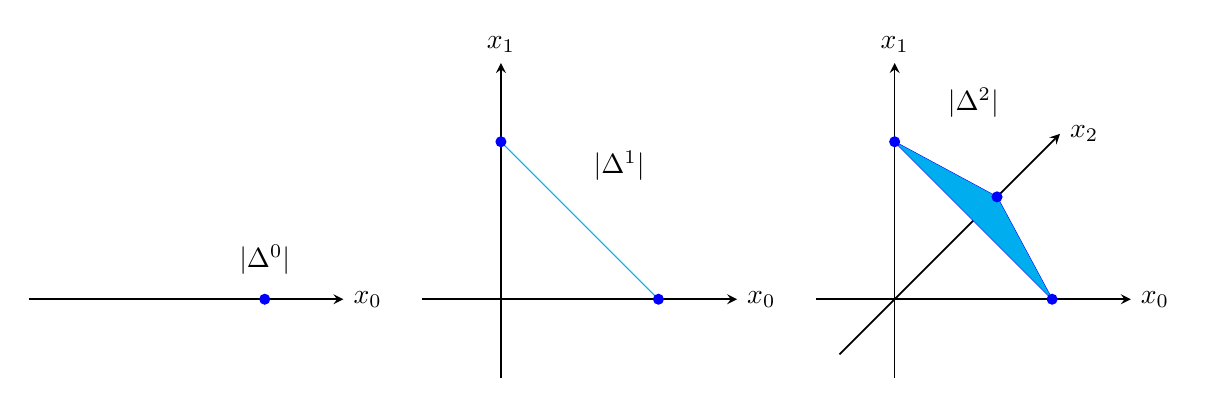
\begin{tikzpicture}
    \node (f0) at (3, 0.5) {$|\Delta^0|$};
    \node (f1) at (7.5,1.7) {$|\Delta^1|$};
    \node (f1) at (12,2.5) {$|\Delta^2|$};
    \draw[semithick,->,>=stealth] (0,0) to (4,0) node[right] {$x_0$};
    \draw[semithick,->,>=stealth] (5,0) to (9,0) node[right] {$x_0$};
    \draw[semithick,->,>=stealth] (6,-1) to (6,3) node[above] {$x_1$};
    \draw[semithick,->,>=stealth] (10,0) to (14,0) node[right] {$x_0$};
    \draw[semithick,->,>=stealth] (11,-1) to (11,3) node[above] {$x_1$};
    \draw[semithick,->,>=stealth] (10.3,-0.7) to (13.1,2.1) node[right] {$x_2$};
    \draw[cyan] (8,0) to (6,2);
    \draw[blue] (13,0) to (11,2) to (12.3,1.3) to cycle;
    \fill[cyan] (13,0) to (11,2) to (12.3,1.3) to cycle;
    \fill[blue] (3,0) circle[radius=2pt]; 
    \fill[blue] (8,0) circle[radius=2pt]; \fill[blue] (6,2) circle[radius=2pt];
    \fill[blue] (13,0) circle[radius=2pt]; \fill[blue] (11,2) circle[radius=2pt]; 
    \fill[blue] (12.3,1.3) circle[radius=2pt];
  \end{tikzpicture} 
\end{center}

位相空間$X$に対して, 連続写像$\si: |\Delta^n| \to X$を$X$の特異$n$単体(singular $n$-simplex)という. 
特異$n$単体は
\begin{align*}
  (d_i\si)(t_0,\cdots,t_{n-1}):= \si(t_0,\cdots,t_{i-1},0,t_i,\cdots,t_{n-1})
\end{align*}
で与えられる特異$(n-1)$単体の集まり$\{d_i\si\}_{0 \leq i \leq n}$を定める. 
この特異$(n-1)$単体は$\si$の面(face)と呼ばれる. 

$X$の特異$n$単体の集合を$\Sing_n(X):= \Hom_{\Top}(|\Delta^n|,X)$とあらわす. 
$X$の重要な代数的不変量は集合$\{\Sing_n(X)\}_{n \geq 0}$と面写像$\{d_i: \Sing_n(X) \to \Sing_{n-1}(X)\}_{0 \leq i \leq n}$から抜き取ることができる. 

\begin{example}
  位相空間$X$に対して, 特異ホモロジー群(singular homology group) $H_{\ast}(X;\Z)$をチェイン複体
  \begin{align*}
    \cdots \xr{\del} \Z[\Sing_1(X)] \xr{\del} \Z[\Sing_0(X)]
  \end{align*}
  のホモロジー群として定義する. 
  ここで$\Z[\Sing_n(X)]$は集合$\Sing_n(X)$から生成される自由Abel群であり, 微分作用素は
  \begin{align*}
    \del(\si):= \sum_{i=0}^{n} (-1)^id_i\si
  \end{align*}
  で定義される. 

  また, 特異$n$単体$\si: |\Delta^n| \to X$は
  \begin{align*}
    (s_i \si)(t_0,\cdots,t_{n+1}):= \si(t_0,\cdots,t_{i-1},t_i+t_{i+1},t_{i+2},\cdots,t_{n+1})
  \end{align*}
  で与えられる特異$(n+1)$-単体の集まり$\{s_i \si\}_{0 \leq i \leq n}$も定める. 
  $s_i \si$であらわされる特異$(n+1)$-単体は線形射影$|\Delta^{n+1}| \to |\Delta^n|$に分解されるので, 構成$s_i: \Sing_n(X) \to \Sing_{n+1}(X)$は退化写像(degeneracy map)と呼ばれる. 
  例えば, 写像$s_0: \Sing_0(X) \to \Sing_1(X)$は各点$x \in X \simeq \Sing_0(X)$を$x$に値をとる定値写像$\uline{x}: |\Delta^1| \to X$に送る. 
\end{example}

\begin{example}
  $X$を基点$x \in X \simeq \Sing_0(X)$を備えた位相空間とする. 
  $p(0)=p(1)=x$を満たす連続な道$p: [0,1] \to X$は集合$\{\si \in \Sing_1(X): d_0(\si)=d_1(\si)=x\}$の元と思える. 
  基本群(fundamental group) $\pi_1(X,x)$とは商集合
  \begin{align*}
    \{\si \in \Sing_1(X): d_0(\si)=d_1(\si)=x\}/\simeq
  \end{align*}
  である. 
  $\simeq$とは次の同値関係
  \begin{align*}
    \si \simeq \si'
    \Leftrightarrow
    \exists \tau \in \Sing_2(X)~ \mathrm{s.t.} ~d_0(\tau)=s_0(x), d_1(\tau)=\si, d_2(\tau)=\si'
  \end{align*}
  である. 
  この条件を満たす$2$単体$\tau$とは連続写像$|\Delta^2| \to X$で, 境界が次のようにふるまうものである. 
  \begin{center}
    \begin{tikzpicture}
      \node (a0) at (0,0) {$x$}; \node (a1) at (1.5,2.5) {$x$}; \node (a2) at (3,0) {$x$}; 
      \draw[->] (a0) to node[left] {$\si'$} (a1); 
      \draw[->] (a1) to node[right] {$\uline{x}$} (a2); 
      \draw[->] (a0) to node[below] {$\si$} (a2); 
    \end{tikzpicture}
  \end{center}
  この写像は$\si$と$\si'$から定まる道の間のホモトピーと思える. 
\end{example}

以上の例から, 次の疑問が自然に生じる. 

\begin{que}
  位相空間$X$に対して, 面写像と退化写像
  \begin{align*}
    d_i: \Sing_n(X) \to \Sing_{n-1}(X),~ s_i: \Sing_n(X) \to \Sing_{n+1}(X)
  \end{align*}
  を備えた集合の集まり$\{\Sing_n(X)\}_{n \geq 0}$について何がいえるだろうか.
  そして, この集まりの数学的構造は何だろうか. 
\end{que}

EilenbergとZilberは\cite{EZ}で完備半単体的複体(complete semi-simplicial complex)を定義して, 疑問1.1.0.3に答えを与えた.
これは今では単体的集合(simplicial set)と呼ばれている. 
大雑把にいうと, 単体的集合$\S$とはいくつかの恒等式を満たす面写像$\{d_i: S_n \to S_{n-1}\}_{0 \leq i \leq n}$と退化写像$\{s_i: S_n \to S_{n+1}\}_{0 \leq i \leq n}$を備えた
$n$で添字つけられた集合の集まり$\{S_n\}_{n \geq 0}$である. 
この恒等式は単体的集合を単体圏(simplex category) $\csim$上の前層と思うことでまとめられる. (1章1節)

単体的集合は次の2つの似通った構成によって, 代数的トポロジーと結びつけられる. 
\begin{itemize}
  \item すべての位相空間$X$に対して, 上で定義した面写像と退化写像は単体的集合の構造をもつ集まり$\{\Sing_n(X)\}_{n \geq 0}$を与える. 
  この単体的集合を$\Sing_\bullet(X)$とあらわし, $X$の特異単体的集合(singular simplicial set)という.
  この単体的集合はとても大きく, 位相空間が離散でない場合には, 集合$\Sing_n(X)$の濃度は非可算となる. 
  \item 任意の単体的集合$\S$から$\S$の幾何学的実現(geometric realization)と呼ばれる位相空間$|\S|$を構成できる. 
  $|\S|$は非交和$\coprod_{n \geq 0}S_n \ti |\Delta^n|$を面写像と退化写像により定まる同値関係で割った商空間である. 
  我々の興味がある位相空間(例えば, 有限回の三角形分割が可能な位相空間)は, 有限の非退化な単体をもつ単体的集合$\S$の幾何学的実現として存在する.
  これは1章2節で議論する. 
\end{itemize}

これらの構成は単体的集合のなす圏$\sset$と位相空間のなす圏$\Top$の間の随伴
\[\begin{tikzcd}
	\sset && \Top
	\arrow["{|-|}", shift left=2, from=1-1, to=1-3]
	\arrow["{\Sing_\bullet}", shift left=2, from=1-3, to=1-1]
\end{tikzcd}\]
を定める. 
これらの関手の構成は1章8節と1章9節で見る. 
\cite[\href{https://kerodon.net/tag/007J}{Tag 007J}]{kerodon}で再び議論する. 

任意の(点付き)位相空間$X$に対して, 例1.1.0.1と例1.1.0.2は$X$の特異ホモロジーと基本群が単体的集合$\Sing_\bullet(X)$から復元できることを示している. 
実際, $X$のすべてのホモトピー型の情報を$\Sing_\bullet(X)$から復元できる. 
正確に言うと, 上で述べた随伴の余単位を考えると自然な写像$|\Sing_\bullet(X)| \to X$が存在する. 
Gieverはこの2つが弱ホモトピー同値であることを示した. 
よって, $X$がCW複体と弱ホモトピー同値であれば, これはホモトピー同値となる. \cite[\href{https://kerodon.net/tag/013X}{Tag 013X}]{kerodon}
ホモトピー論を勉強するためには, $X$を$\Sing_\bullet(X)$に変えて, 位相空間論ではなく単体的集合の状況で考えても問題はない.
実際, 代数的トポロジーの理論を$X$から誘導される単体的集合をもちいて, 組み合わせ論的な議論に置き換えることができる. 
しかし, すべての単体的集合が位相空間の特異複体のようにふるまうわけではない. 
よって, 議論をするためには「いい」単体的集合のクラスに制限する必要がある. 
1章9節でKan複体(Kan complex)と呼ばれる単体的集合を定義する. 
Milnorは\cite{MJ2}で, CW複体の古典的なホモトピー論とKan複体のホモトピー論が同値であることを示した. 
このことは\cite[\href{https://kerodon.net/tag/00SY}{Tag 00SY}]{kerodon}で再び議論する. 

\subsection{単体的対象と余単体的対象}

\begin{nota}
  任意の$n$に対して, 線形順序集合$\{0 < 1<, \cdots,< n\}$を$[n]$とあらわす. 
\end{nota}  

\begin{definition}
  圏$\csim$を次のように定義する. 
  \begin{itemize}
    \item $\csim$の対象は$[n]$の形であらわされる線形順序集合
    \item $[m]$から$[n]$への射は非減少な写像$\al: [m] \to [n]$, つまり$0 \leq i \leq j \leq m$に対して, $0 \leq \al(i) \leq \al(j) \leq n$となるような写像
  \end{itemize}
  圏$\csim$を単体圏(simplex category)という. 
\end{definition} 

\begin{remark}
  圏$\csim$は(空でない)すべての有限線形順序集合と非減少な写像のなす圏と圏同値である. 
\end{remark} 

\begin{Proof}
  任意の(空でない)有限線形順序集合$I$に対して, 順序を保つ全単射$I \simeq [n]$が一意に存在するようなある$n$が存在することから従う. 
\end{Proof}

\begin{definition}
  $\calC$を圏とする.
  関手$\simop \to \calC$を$\calC$の単体的対象(simplicial object)という. \\
  双対的に, 関手$\csim \to \calC$を$\calC$の余単体的対象(cosimplicial object)という. 
\end{definition}

\begin{nota}
  圏$\calC$の単体的対象を$C_{\bullet}$, 対象$[n] \in \csim$における関手$C_{\bullet}$の値を$C_n$とあらわす. \\
  同様に, 圏$\calC$の余単体的対象を$C^{\bullet}$, 対象$[n] \in \csim$における関手$C^{\bullet}$の値を$C^n$とあらわす. 
\end{nota} 

\begin{definition}
  対象が$[n]$の形であらわされる線形順序集合, 射が狭義増加関数$\al: [m] \hookrightarrow [n]$である圏を$\insim$とあらわす. 
  $\calC$を圏とする. 
  関手$\insimop \to \calC$を$\calC$の半単体的対象(semi-simplicial object)という. 
  $\calC$の半単体的対象を$C_{\bullet}$, 対象$[n] \in \insimop$における関手$C_{\bullet}$の値を$C_n$とあらわす. 
\end{definition}

\begin{remark}
  圏$\insim$は圏$\csim$の(充満ではない)部分圏とみなせる. 
  圏$\calC$の単体的対象$C_{\bullet}$から合成
  \begin{align*}
    \insimop \hookrightarrow \simop \xr{C_{\bullet}} \calC
  \end{align*}
  によって圏$\calC$の半単体的対象が定まる.
\end{remark}

単体的対象$C_{\bullet}$は対象$\{C_n\}_{n \geq 0}$の集まりとみなせるが, 単体圏$\csim$における射から生じる追加の構造が備わっている. 

\begin{nota}
  $n \geq 1$と$0 \leq i \leq n$に対して, $\delta^i: [n-1] \to [n]$を次のように定義する.
  \begin{align*}
    \delta^i(j) :=
    \begin{cases}
      j & (j < i) \\
      j+1 & (j \geq i)
    \end{cases}
  \end{align*} 
  これは像に元$i$を含まない狭義増加写像(つまり, 単射)である. \\
  $C_{\bullet}$を圏$\calC$の(半)単体的対象とする. 
  射$\delta^i$を$C_{\bullet}$で送ると, 射$C_n \to C_{n-1}$が得られる. 
  この写像を$d_i: C_n \to C_{n-1}$とあらわし, $i$番目の面写像($i$-th face map)という. \\
  $C^{\bullet}$を圏$\calC$の余単体的対象とする. 
  双対的に, 射$\delta^i$を$C^{\bullet}$で送ると, 射$C^{n-1} \to C^n$が得られる. 
  この写像を$d^i: C^{n-1} \to C^n$とあらわし, $i$番目の余面写像($i$-th coface map)という.
\end{nota}

\begin{nota}
  $0 \leq i \leq n$に対して, $\si^i: [n+1] \to [n]$を次のように定義する.
  \begin{align*}
    \si^i(j) :=
    \begin{cases}
      j & (j \leq i) \\
      j-1 & (j > i)
    \end{cases}
  \end{align*} 
  これは像に元$i$が重複する全射である. \\
  $C_{\bullet}$を圏$\calC$の単体的対象とする. 
  射$\si^i$を$C_{\bullet}$で送ると, 射$C_n \to C_{n+1}$が得られる. 
  この写像を$s_i: C_n \to C_{n+1}$とあらわし, $i$番目の退化写像($i$-th degeneracy map)という. \\
  双対的に, $C^{\bullet}$を圏$\calC$の余単体的対象とする. 
  射$\si^i$を$C^{\bullet}$で送ると, 射$C^{n+1} \to C^n$が得られる. 
  この写像を$s^i: C^{n+1} \to C^n$とあらわし, $i$番目の余退化写像($i$-th codegeneracy map)という.
\end{nota}

\begin{exe}
  $C_{\bullet}$を圏$\calC$の半単体的対象とする. 
  このとき, 面写像が次の条件
  \begin{itemize}
    \item[$(\ast)$] $n \geq 2$と$0 \leq i < j \leq n$に対して, $C_n$から$C_{n-2}$への写像として$d_i \ci d_j = d_{j-1} \ci d_i$
  \end{itemize}
  を満たすことを示せ. \\
  逆に, 条件$(\ast)$を満たす任意の対象の集まり$\{C_n\}_{n \geq 0}$と射$\{d_i: C_n \to C_{n-1}\}_{0 \leq i \leq n}$は一意に$\calC$の半単体的対象を決定することを示せ. 
\end{exe} 

\begin{Proof}
  前半は計算すれば分かる. \\
  後半は圏$\insim$の任意の射が$\delta$の合成で一意にあらわせて, 上の関係式を満たすことから分かる. 
\end{Proof}  

\begin{exe}
  $C_{\bullet}$を圏$\calC$の単体的対象とする. 
  面写像と退化写像が単体的恒等式(simplicial identities)と呼ばれる次の条件
  \begin{enumerate}
    \item $n \geq 2$と$0 \leq i < j \leq n$に対して, $C_n$から$C_{n-2}$への写像として$d_i \ci d_j = d_{j-1} \ci d_i$
    \item $0 \leq i \leq j \leq n$に対して, $C_n$から$C_{n+2}$への写像として$s_i \ci s_j = s_{j+1} \ci s_i$
    \item $0 \leq i,j \leq n$に対して, 
    \begin{align*}
      d_i \ci s_j =
      \begin{cases}
        s_{j-1} \ci d_i & (i < j) \\
        \id_{C_n} & (i=j,j+1) \\
        s_j \ci d_{i-1} & (i > j+1) 
      \end{cases}
    \end{align*}
  \end{enumerate} 
  を満たすことを示せ. \\
  逆に, 条件(1), (2), (3)を満たす任意の対象の集まり$\{C_n\}_{n \geq 0}$と射の集まり
  $\{d_i: C_n \to C_{n-1}\}_{0 \leq i \leq n}$, $\{s_i: C_n \to C_{n+1}\}_{0 \leq i \leq n}$は一意に$\calC$の単体的対象を決定することを示せ.
\end{exe}

\begin{Proof}
  前半は計算すれば分かる. \\
  後半は圏$\csim$の任意の射が$\delta$と$\si$の合成で一意にあらわせて, (1)から(3)までの関係式を満たすことから分かる. 
\end{Proof}

単体的対象で重要な例は次の単体的集合である. 

\begin{definition}
  集合と写像のなす圏を$\cset$とあらわす. 
  単体的集合(simplicial set)とは$\cset$の単体的対象, つまり関手$\simop \to \cset$である. 
  半単体的集合(semi-simplicial set)とは$\cset$の半単体的対象, つまり関手$\insimop \to \cset$である. \\
  $\S$を(半)単体的集合とする. 
  このとき, $S_n$の元を$n$単体($n$-simplex)という. 
  特に, $S_0$の元を$\S$の点(vertex), $S_1$の元を$\S$の辺(edge)という.  
\end{definition}

$\simop$から$\cset$への関手のなす圏を$\sset$とあらわす. 
$\sset$を単体的集合のなす圏(category of simplicial sets)という. 

\begin{remark}
  集合のなす圏$\cset$は完備かつ余完備なので, (半)単体的集合のなす圏も完備かつ余完備である. 
  \footnote{
    $\calJ$が小圏で$\calC$が余完備なら, $\fun(\calJ,\calC)$も余完備である. 
    双対的に, $\calJ$が小圏で$\calC$が完備なら, $\fun(\calJ,\calC)$も完備である. 
  }
  更に, 極限と余極限は各点で計算することができる. 
  つまり, 次の関手
  \begin{align*}
    \S: \calC \to \sset: C \mt \S(C)
  \end{align*}
  に対して, 自然な全単射
  \begin{align*}
    (\varinjlim_{C \in \calC}S(C))_n \simeq \varinjlim_{C \in \calC}(S_n(C)) \\
    (\varprojlim_{C \in \calC}S(C))_n \simeq \varprojlim_{C \in \calC}(S_n(C))
  \end{align*}
  が存在する. 
\end{remark}

\subsection{標準単体とホーン}

単体的集合の基本的な例をいくつか見よう. 

\begin{cons}
  米田埋め込み$y:\csim \to \sset$に対して, $\Delta^n:=y([n]) \in \sset$とあらわして, 標準$n$単体(standard $n$-simplex)という.
  つまり, $\Delta^n$は
  \begin{align*}
    [-] \mt \Hom_{\csim}([-],[n])
  \end{align*}
  で与えられる. 
  形式的に$\Delta^{-1}:=\emptyset$と定義して, この構成を$n=-1$の場合にも拡張する. 
\end{cons}

\begin{example}
  $\csim$の終対象は$[0]$であり, 米田埋め込み$y$は極限を保つので, 標準$0$単体$\Delta^0$は単体的集合のなす圏における終対象である. 
\end{example}

\begin{remark}
  標準$n$単体$\Delta^n$は次の普遍性で特徴づけられる. 
  任意の単体的集合$X_{\bullet}$に対して, 米田の補題より全単射
  \begin{align*}
    \Hom_{\sset}(\Delta^n,X_{\bullet}) \simeq X_n
  \end{align*}
  が存在する. 
  よって, $X_{\bullet}$の$n$単体を単体的集合の間の写像$\si: \Delta^n \to X_{\bullet}$と同一視する. 
\end{remark}

\begin{remark}
  $\S$を単体的集合とする. 
  任意の$n$に対して, 部分集合$T_n \subset S_n$が与えられていて, 面写像と退化写像
  \begin{align*}
    d_i: S_n \to S_{n-1}, ~ s_i: S_n \to S_{n+1}
  \end{align*}
  が$T_n$をそれぞれ$T_{n-1}$と$T_{n+1}$にうつすとする. 
  練習1.1.1.11より, 集まり$\{T_n\}_{n \geq 0}$は単体的集合$T_{\bullet}$の構造をもつ. 
  このとき, $T_{\bullet}$を$\S$の単体的部分集合(simplicial subset)といい, $T_{\bullet} \subset \S$とあらわす. 
\end{remark}

\begin{example}
  $\S$を単体的集合, $\nu$を$\S$の点とする. 
  米田の補題より, $\nu$は単体的集合の間の写像$\Delta^0 \to \S$と同一視できる. 
  任意の$n$に対して$\Delta^0$はただ1つの$n$単体をもつので, この写像はモノ射である. 
  この写像の像は$\S$の単体的部分集合であり, $\{\nu\}$とあらわす. 
  例えば, 標準$n$単体$\Delta^n$の点は$0 \leq i \leq n$を満たす整数$i$と同一視できる. 
  そのような$i$は($k$単体が$i$に値をとる定値写像$[k] \to [n]$となる)単体的部分集合$\{i\} \subset \Delta^n$を定めるからである. 
\end{example}

% 米田の補題より, 全単射
% \begin{align*}
%   \Delta^n_0 \to \Hom_{\sset}(\Delta^0,\Delta^n): \nu \mt 
% \end{align*}

他にも標準$n$単体の単体的部分集合の例を見る. 

\begin{cons}
  単体的集合$\del \Delta^n: \simop \to \cset$を次のように定義する. 
  \begin{align*}
    \del \Delta^n([-]):= \{\al \in \Hom_{\csim}([-],[n]): \al \text{は全射でない}\}
  \end{align*}
  $\del \Delta^n$は標準$n$単体$\Delta^n$の単体的部分集合とみなせる. 
  $\del \Delta^n$を$\Delta^n$の境界(boundary)という. 
\end{cons}

\begin{example}
  単体的集合$\del \Delta^0$は空である. 
\end{example}

\begin{exe}
  
\end{exe}

\begin{cons}
  $0 \leq i \leq n$に対して, 単体的集合$\Lambda^n_i: \simop \to \cset$を次のように定義する. 
  \begin{align*}
    \Lambda^n_i([-]):= \{\al \in \Hom_{\csim}([-],[n]):~ [n] \not\subset \al([-]) \cup \{i\}\}
  \end{align*}
  $\Lambda^n_i$は境界$\del \Delta^n \subset \Delta^n$の単体的部分集合とみなせる. 
  $\Lambda^n_i$を$\Delta^n$の$i$番目のホーン($i$-th horn)という. 
  $0<i<n$のときは$\Lambda^n_i$を内部ホーン(inner horn), $i=0,n$のときは外部ホーン(outer horn)という. 
\end{cons}

\begin{remark}
  大雑把にいうと, 境界$\del \Delta^n$は 標準$n$単体$\Delta^n$から内部を抜き取ったもの, 
  ホーン$\Lambda^n_i$は境界$\del \Delta^n$から$i$-番目の点と向かい合う面(the face opposite its $i$-th vertex)を抜き取ったものと思える. 
\end{remark}

\begin{example}
  $\Delta^2$から得られるホーンは次のように描くことができる. 
  \begin{center}
    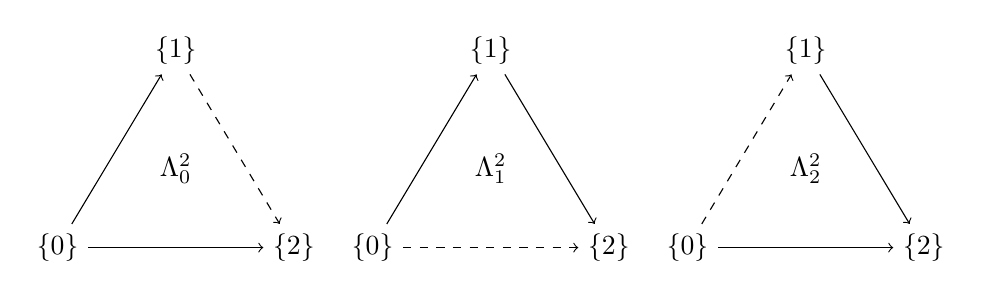
\begin{tikzpicture}
      \node (a0) at (0,0) {$\{0\}$}; \node (a1) at (1.5,2.5) {$\{1\}$}; \node (a2) at (3,0) {$\{2\}$}; 
      \node (c1) at (1.5,1.0) {$\Lambda^2_0$};
      \draw[->] (a0) to (a1); 
      \draw[->, dashed] (a1) to (a2); 
      \draw[->] (a0) to (a2); 
      \node (b0) at (4,0) {$\{0\}$}; \node (b1) at (5.5,2.5) {$\{1\}$}; \node (b2) at (7,0) {$\{2\}$}; 
      \node (c2) at (5.5,1.0) {$\Lambda^2_1$};
      \draw[->] (b0) to (b1); 
      \draw[->] (b1) to (b2); 
      \draw[->, dashed] (b0) to (b2); 
      \node (d0) at (8,0) {$\{0\}$}; \node (d1) at (9.5,2.5) {$\{1\}$}; \node (d2) at (11,0) {$\{2\}$}; 
      \node (c3) at (9.5,1.0) {$\Lambda^2_2$};
      \draw[->, dashed] (d0) to (d1); 
      \draw[->] (d1) to (d2); 
      \draw[->] (d0) to (d2);
    \end{tikzpicture}
  \end{center}
  ただし, 点線はその辺が「含まれていない」ことを表している. 
\end{example}

\begin{Proof}
  証明は\cite{Alg-d}の2章3節を参照.
  一般化は定義1.1.8.7と例1.1.8.9を参照. 
\end{Proof}

\begin{example}
  ホーン$\Lambda^1_0$と$\Lambda^1_1$はともに$\Delta^0$と同型である. 
  包含写像$\Lambda^1_0 \hookrightarrow \del \Delta^1 \hookleftarrow \Lambda^1_1$は同型
  \begin{align*}
    \del \Delta^1 \simeq \Lambda^1_1 \sqcup \Lambda^1_1 \simeq \Delta^0 \sqcup \Delta^0
  \end{align*}
  を誘導する. 
\end{example}

\begin{example}
  ホーン$\Lambda^0_0$は空である. 
  よって, 境界$\del \Delta^0$と一致する. 
\end{example}

\begin{exe}
  
\end{exe}

\subsection{骨格的フィルトレーション}

大雑把にいうと, 単体的集合$\Delta^n$は複雑な単体的集合を構成する基本的な構成要素である. 
この節では, 単体的集合の骨格的フィルトレーション(skeletal filtration)を定義して, 厳密に説明する. 
フィルトレーションによって任意の単体的集合を単体的部分集合の増大列
\begin{align*}
  \sk_0(\S) \subset \sk_1(\S) \subset \sk_2(\S) \subset \cdots
\end{align*}
の和集合であらわすことができる. 
ここで, $\sk_n(\S)$は$\sk_{n-1}(\S)$に$\Delta^n$のコピーを貼り合わせることで得られる. 

\begin{prop}
  $n>0$, $\tau \in S_n$を単体的集合$\S$の$n$単体とする. 
  米田の補題より, 単体的集合の間の写像$\tau: \Delta^n \to \S$と同一視する. 
  このとき, 次の5つは同値である.
  \begin{enumerate}
    \item ある$0 \leq i \leq n-1$に対して, $\tau$は退化写像$s_i: S_{n-1} \to S_n$の像の元である. 
    
    \item $\tau$は合成$\Delta^n \xr{f} \Delta^{n-1} \to \S$に分解される. 
    ここで$f$は全射$[n] \to [n-1]$から誘導される写像$\Delta^n \to \Delta^{n-1}$である. 
    
    \item $\tau$はある$m < n$に対して, 合成$\Delta^n \xr{f} \Delta^m \to \S$に分解される. 
    ここで$f$は全射$[n] \to [m]$から誘導される写像$\Delta^n \to \Delta^m$である. 
    
    \item $\tau$は$m<n$に対して, 合成$\Delta^n \to \Delta^m \to \S$に分解される. 
    
    \item $\tau$は合成$\Delta^n \xr{\tau'} \Delta^m \to \S$に分解される. 
    ここで$\tau'$は点に対して, 単射ではない写像である. 
  \end{enumerate} 
\end{prop}

\begin{Proof}
  (1)から(2)を示す. 
  対応する$\Delta^{n-1} \to \S$, つまり$S_{n-1}$の元が存在することから, $\tau$が$\Delta^n \xr{f} \Delta^{n-1} \to \S$のように分解されることから分かる. 
  (2)から(1)は$\Delta^{n-1} \to \S$に$f: \Delta^n \to \Delta^{n-1}$を合成すれば$\Delta^n \to \S$が得られることから分かる.
  (2)から(3)と(3)から(4)は明らかである.  
  (4)から(5)は$m < n$なので, $\tau'$は点に対して単射ではないことから分かる. 
  あとは(5)から(1)を示せばよい. 
  $\tau$が点に関して単射ではない写像$\tau'$を用いて, 合成$\Delta^n \xr{\tau'} \Delta^m \to \S$に分解されるとする. 
  このとき, $\tau'(i)=\tau'(i+1)$を満たすある$i ~(0<i<n)$が存在する. 
  つまり, $\tau'$は$\si^i: [n] \to [n-1]$から誘導される写像$\Delta^n \to \Delta^{n-1}$に分解される. 
  よって, $\tau$は退化写像$s_i$の像の元である. 
\end{Proof}

\begin{definition}
  $\si: \Delta^n \to \S$を単体的集合$\S$の$n$単体とする. 
  $n>0$に対して, $\si$が命題1.1.3.1の条件を満たしているとき, $\si$は退化である(degenerate)という. 
  $\si$が退化でないとき, 非退化である(nondegenerate)という. 
  例えば, すべての$0$単体は非退化である. 
\end{definition}

\begin{remark}
  $f: \S \to \T$を単体的集合の間の写像とする. 
  $\si$が$\S$の退化な$n$単体であるとする. 
  このとき, $f(\si)$は$\T$の退化な$n$単体である. 
  逆は$f$がモノ射であるときに限り成立する. 
  例えば, $\S$が$\T$の単体的部分集合であり, $f$が包含写像であるときである.
\end{remark}

\begin{Proof}
  $m<n$とする. 
  全射$[n] \to [m]$から誘導される写像を$\al: \Delta^n \to \Delta^m$とする. 
  $\si$は$\S$の退化な$n$単体なので, $\Delta^n \xr{\al} \Delta^m \xr{\tau} \S$と分解できる. 
  この$m$単体$\tau: \Delta^m \to \S$を$f$で送ると, $f(\tau): \Delta^m \to \T$となる. 
  $f$は自然変換なので, 次の図式は可換である. 
  \[\begin{tikzcd}
    {S_m} & {T_m} && {(\Delta^m \to \S)} & {(\Delta^m \to \T)} \\
    {S_n} & {T_n} && {(\Delta^n \to \S)} & {(\Delta^n \to \T)}
    \arrow[from=1-1, to=2-1]
    \arrow[from=1-2, to=2-2]
    \arrow[from=2-1, to=2-2]
    \arrow["{- \ci \al}"', maps to, from=1-4, to=2-4]
    \arrow["{f \ci -}", maps to, from=1-4, to=1-5]
    \arrow["{- \ci \al}", maps to, from=1-5, to=2-5]
    \arrow[from=1-1, to=1-2]
    \arrow["{f \ci -}"', maps to, from=2-4, to=2-5]
  \end{tikzcd}\]
  つまり, $f(\tau) \ci \al=f(\tau \ci \al) = f(\si)$が成立する. 
  よって, $\T$の$n$単体$f(\si): \Delta^n \to \T$は$\Delta^n \xr{\al} \Delta^m \xr{f(\tau)} \T$に分解される. \\
  逆を示す. 
  $f(\si): \Delta^n \to \S \to \T$は仮定より非退化であるので, ある$m < n$を用いて$\Delta^n \xr{\al} \Delta^m \xr{\tau} \S \xr{f} \T$と分解される. 
  ここで$\al$は全射$[n] \to [m]$から誘導される写像$\al: \Delta^n \to \Delta^m$であり, $\tau$は非退化な$m$単体である. 
  $f$はモノ射であるので, $\Delta^n \xr{\al} \Delta^m \xr{\tau} \S$と$\Delta^n \xr{\si} \S$は一致する. 
  つまり, $\si$は$\S$の退化な$n$単体である. 
\end{Proof}

\begin{prop}[Eilenberg-Zilberの補題]
  $\si: \Delta^n \to \S$を単体的集合の間の写像とする. 
  このとき, $\si$は合成 
  \begin{align*}
    \Delta^n \xr{\al} \Delta^m \xr{\tau} \S
  \end{align*}
  に一意に分解できる. 
  ここで$\al$は全射$[n] \to [m]$から誘導される写像, $\tau$は$\S$の非退化な$m$-単体である. 
\end{prop}

\begin{Proof}
  まずは存在性を示す. 
  $\si$が非退化であるとき, $m=n$として$\Delta^n \to \Delta^n$を$\id_{[n]}: [n] \to [n]$から誘導される写像, $\Delta^m \to \S$を$\si: \Delta^n \to \S$とすればよい. 
  $\si$が退化であるとき, 命題1.1.3.1より分解$\Delta^n \xr{\al} \Delta^m \xr{\tau} \S$と分解できる. 
  ここで$m$はこのような分解ができる最小の整数とする. 
  (そうでない場合は$[m]$を$\al$を誘導する写像の像からなる線形順序集合に置き換えればよい.)
  このとき, $\tau$は非退化である.  
  次に一意性を示す. 
  全射$[n] \to [m']$から誘導される写像$\al': \Delta^n \to \Delta^{m'}$と非退化な$m'$単体$\tau': \Delta^{m'} \to \S$を用いて, $\si$が$\Delta^n \xr{\al'} \Delta^{m'} \xr{\tau'} \S$と分解されたとする. 
  $\al'(i)=\al'(j)$を満たす$i$と$j$に対して, $\al(i)=\al(j)$が成立することを示す. 
  仮に$\al(i) \neq \al(j)$とすると, $\al$は切断$\beta: \Delta^m \hookrightarrow \Delta^n$をもつ. 
  このとき, 
  \begin{align*}
    \tau 
    = \tau \ci \al \ci \beta
    = \si \ci \beta
    = \tau' \ci \al' \ci \beta
  \end{align*}
  である. 
  $\al'(i)=\al'(j)$より, 写像$\al' \ci \beta: \Delta^m \to \Delta^{m'}$は点に対して単射ではない. 
  これは$\tau$が非退化であることに反する. 
  よって, $\al$は点に関して全射でもある$\al'': \Delta^{m'} \to \Delta^m$を用いて, $\Delta^n \xr{\al'} \Delta^{m'} \xr{\al''} \Delta^m$と一意に分解される. 
  $\al'$の切断を$\beta': \Delta^{m'} \hookrightarrow \Delta^n$とすると, 
  \begin{align*}
    \tau'
    = \tau' \ci \al' \ci \beta'
    = \si \ci \beta'
    = \tau \ci \al \ci \beta'
    = \tau \ci \al'' \ci \al' \ci \beta'
    = \tau \ci \al''
  \end{align*}
  となる. 
  $\tau'$が非退化であるとすると, $\al''$は点に対して単射である. 
  つまり, $m=m'$であり, $\al''$は恒等射である. 
  $\al=\al', \tau=\tau'$であるので, 一意性は示された. 
\end{Proof}

\begin{cons}
  $\si: \Delta^n \to \S$を単体的集合$\S$の$n$単体, $k \geq -1$とする. 
  命題1.1.3.4より, 次の2つは同値である. 
  \begin{enumerate}
    \item $\Delta^n \xr{\al} \Delta^m \xr{\tau} \S$を命題1.1.3.4の分解とする. 
    このとき, $m \leq k$である. 
    \item ある$m' \leq k$に対して, 分解$\Delta^n \to \Delta^{m'} \to \S$が存在する. 
  \end{enumerate}
\end{cons}

\begin{Proof}
  (1)から(2)は明らか. 
  (2)から(1)は命題1.1.3.4そのものである. 
\end{Proof}

(1)か(2)を満たす$n$単体を含む$S_n$の部分集合を$\sk_k(S_n)$とあらわす. 
(2)の条件より, 部分集合の集まり$\{\sk_k(S_n)\}_{n \geq 0}$は面写像と退化写像で安定である. 
よって, 注意1.1.2.4より, $\{\sk_k(S_n)\}_{n \geq 0}$は単体的部分集合を定める. 
この単体的部分集合を$\sk_k(\S)$とあらわし, $\S$の$k$骨格($k$-skeleton)という. 

\begin{remark}
  $\S$を単体的集合, $k \geq -1$とする. 
  $n \leq k$であれば, 定義より$\sk_k(\S)$は$\S$のすべての$n$単体を含む. 
  特に, 和集合$\bigcup_{k \geq 1} \sk_k(\S)$は$\S$に等しい. 
\end{remark}

\begin{remark}
  $\si: \Delta^n \to \S$を単体的集合$\S$の非退化な$n$単体とする.
  このとき, $\si$が$\sk_k(\S)$に含まれる必要十分条件は$n \leq k$である.
\end{remark}

\begin{Proof}
  必要条件を示す. 
  $\si$は非退化なので分解ができない. 
  よって, 構成1.1.3.5において$m=n$であるので, $n \leq k$が成立する. 
  十分条件は注意1.1.3.6より成立する.
\end{Proof}

\begin{example}
  任意の単体的集合$\S$に対して, $(-1)$骨格$\sk_{-1}(\S)$は空である. 
\end{example}

\begin{Proof}
  構成1.1.2.1より, $\Delta^{-1}=\emptyset$なので$\Delta^n \to \emptyset$は存在しない.
  よって, 分解ができるような写像の集まりは空である. 
\end{Proof}

単体的集合$\S$の$k$骨格は普遍性を用いて特徴づけることができる. 

\begin{definition}
  $\S$を単体的集合, $k \geq -1$とする. 
  $n>k$に対して, $\S$の任意の$n$単体が退化であるとき, $\S$は次元$\leq k$である($\S$ has dimension $\leq k$)という. 
  $k \geq 0$とする. 
  次元$\leq k$であり, 次元$\leq k-1$でない
  \footnote{
    つまり, 非退化な$k$単体が少なくとも1つ存在するときである. 
  }
  とき, $\S$は次元$k$である($\S$ has dimension $k$)という. 
  $k \gg 0$とする. 
  次元$\leq k$のとき, $\S$は有限次元的である($\S$ is finite-dimensional)という.
\end{definition}

\begin{prop}
  $\S$を単体的集合, $k \geq -1$とする. 
  このとき, 次の2つが成立する. 
  \begin{enumerate}
    \item 単体的集合$\sk_k(\S)$は次元$\leq k$である. 
    \item 次元$\leq k$である任意の単体的集合$\T$に対して, 包含写像$\sk_k(\S) \hookrightarrow \S$は全単射 
    \begin{align*}
      \Hom_{\sset}(\T,\sk_k(\S)) \to \Hom_{\sset}(\T,\S)
    \end{align*}
    を誘導する. 
    つまり, 任意の写像$\T \to \S$の像は$\sk_k(\S)$に含まれる.
  \end{enumerate}
\end{prop}

\begin{Proof}
  (1)は注意1.1.3.7より分かる. 
  (2)を示す. 
  $\T$が次元$\leq k$である単体的集合とする. 
  写像$f: \T \to \S$が$\T$の任意の$n$単体$\si$を$\sk_k(\S)$の$n$単体にうつすことを示す. 
  注意1.1.3.3より, $\si$が退化な場合は$f$で送っても退化である. 
  あとは$\si$が非退化な場合を考えればよい. 
  $\T$は次元$\leq k$であるので, 注意1.1.3.7より$n \leq k$である. 
  注意1.1.3.6より, $f(\si)$は$\sk_k(\S)$に属する. 
\end{Proof}

\begin{prop}
  $\S^-,\S^+$をそれぞれ次元$\leq k_-, \leq k_+$である単体的集合とする. 
  このとき, 直積$\S^- \ti \S^+$は次元$\leq k_- + k_+$である. 
\end{prop}

\begin{Proof}
  
\end{Proof}

\begin{exe}
  $\S^-,\S^+$をそれぞれ次元$\leq k_-, \leq k_+$である単体的集合とする. 
  このとき, 直積$\S^- \ti \S^+$は次元$k_- + k_+$である. 
\end{exe}

$\S$を単体的集合, $k \geq 0$とする. 
$\S$の非退化な$k$単体の集まりを$\snd$とあらわす. 
$\snd$の任意の元$\si$は単体的集合の間の写像$\Delta^k \to \sk_k(\S)$を定める. 
\footnote{
  $\sk_k(\S)$は$k$単体以下のすべての単体を含んでいる. 
  $\snd$の元$\si: \Delta^k \to S^{\mathrm{nd}}_{\bullet}$と包含写像$S^{\mathrm{nd}}_{\bullet} \hookrightarrow \sk_k(\S)$の合成から, 
  単体的集合の間の写像$\Delta^k \to \sk_k(\S)$が定まる. 
}
境界$\del \Delta^k \subset \Delta^k$は次元$\leq k-1$であるので, 命題1.1.3.10より, この写像は$\del \Delta^k$を$(k-1)$骨格$\sk_{k-1}(\S)$にうつす. 

\begin{prop}
  $\S$を単体的集合, $k \geq 0$とする. 
  このとき, 上の構成は単体的集合のなす圏$\sset$において, 次のプッシュアウトの図式
  \[\begin{tikzcd}
    {\coprod_{\si \in \snd} \del \Delta^k} & {\coprod_{\si \in \snd} \Delta^k} \\
    {\sk_{k-1} (\S)} & {\sk_k(\S)}
    \arrow[from=1-1, to=1-2]
    \arrow[hook, from=1-1, to=2-1]
    \arrow[from=2-1, to=2-2]
    \arrow[from=1-2, to=2-2]
  \end{tikzcd}\]
  を定める. 
\end{prop}

\begin{Proof}
  
\end{Proof}

\subsection{離散単体的集合}

次元$\leq 0$の単体的集合は簡単に分類することができる. 

\begin{prop}
  評価関手(evaluation functor)
  \begin{align*}
    \eva_0: \sset \to \cset: X_{\bullet} \mt X_0
  \end{align*}
  を制限すると, 圏同値
  \begin{align*}
    \{\text{次元}\leq 0 \text{の単体的集合}\} \simeq \cset
  \end{align*}
  が得られる. 
\end{prop}

命題1.1.4.1の証明はこの節の最後で与える.
まずは一般の単体的対象に対して議論する. 

\begin{cons}
  $\calC$を圏とする. 
  各対象$C \in \calC$に対して, $C$に値をとる定値関手$\simop \to \{C\} \hookrightarrow \calC$を$\uline{C}_{\bullet}$とあらわす. 
  これを$\calC$の単体的対象とみなし, $C$に値をとる定数単体的対象(constant simplicial object with value $C$)という. 
\end{cons}

\begin{remark}
  $C$を圏$\calC$の対象とする. 
  定数単体的対象$\uline{C}_\bullet$は次のように書き下すことができる. 
  \begin{itemize}
    \item 各$n$に対して, $\uline{C}_n=C$
    \item 面写像と退化写像 
    \begin{align*}
      d_i: \uline{C}_n \to \uline{C}_{n-1} ~ s_i: \uline{C}_n \to \uline{C}_{n+1}
    \end{align*}
    は$C$から$C$への恒等写像である. 
  \end{itemize}
\end{remark}

\begin{example}
  $S=\{\ast\}$を1元集合とする. 
  このとき, $\uline{S}_{\bullet}: \simop \to \{S\} \hookrightarrow \cset$は単体的集合のなす圏の終対象である.
  \footnote{
    圏$\calC$が終対象$1$を持つとき, 小圏$\calJ$に対して, $\fun(\calJ,\calC)$の終対象は$1$に値をとる定数関手である. 
    今回の場合, 圏$\cset$の終対象は1元集合$S$であるので, $\fun(\simop,\cset)=\sset$の終対象は$\uline{S}_{\bullet}$である. 
  } 
  終対象は同型をのぞいて一意なので, $\uline{S}_{\bullet}$は$\Delta^0$と同型である. 
\end{example}

\begin{prop}
  $C$を圏$\calC$の対象とする. 
  $\calC$の任意の単体的対象$X_{\bullet}$に対して, 自然な写像
  \begin{align*}
    \Hom_{\fun(\simop,\calC)}(\uline{C}_{\bullet},X_{\bullet}) \to \Hom_{\calC}(\uline{C}_0,X_0) = \Hom_{\calC}(C,X_0)
  \end{align*}
  は全単射である.  
\end{prop}

\begin{Proof}
  $f: C \to X_0$を$\calC$における射とする. 
  この$f$から一意に単体的集合の間の写像$f_{\bullet}: \uline{C}_{\bullet} \to X_{\bullet}$を構成すればよい. 
  この写像の一意性は明らかであるので, 存在性を示す. 
  $[n] \in \simop$に対して, 各$f_n$を合成
  \begin{align*}
    f_n: \uline{C}_n = C \xr{f} X_0 \xr{X_{\al(n)}} X_n
  \end{align*}
  と定義する. 
  ここで$\al(-)$は$[-]$から$[0]$への一意な射である. 
  $f_\bullet$が自然変換であることを確かめるために, 任意の非減少関数$\beta: [m] \to [n]$に対して, 次の図式を考える. 
  \begin{center}
    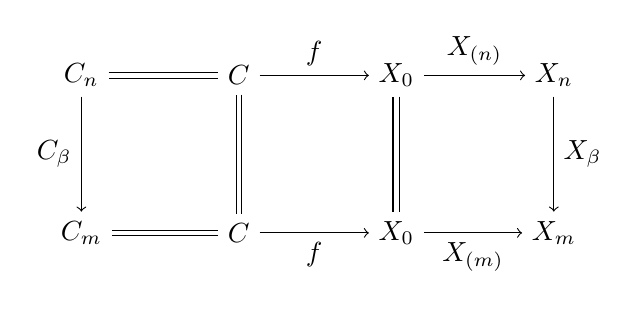
\begin{tikzpicture}
      \node (n0) at (0,2) {$\uline{C}_n$}; \node (n1) at (2,2) {$C$}; \node (n2) at (4,2) {$X_0$}; \node (n3) at (6,2) {$X_n$};  
      \node (m0) at (0,0) {$\uline{C}_m$}; \node (m1) at (2,0) {$C$}; \node (m2) at (4,0) {$X_0$}; \node (m3) at (6,0) {$X_m$}; 
      \draw[->] (n1) to node[above] {$f$} (n2) ; \draw[->] (n2) to node[above] {$X_{\al(n)}$} (n3); 
      \draw[->] (m1) to node[below] {$f$} (m2) ; \draw[->] (m2) to node[below] {$X_{\al(m)}$} (m3); 
      \draw[->] (n0) to node[left] {$\uline{C}_\beta$} (m0) ; \draw[->] (n3) to node[right] {$X_\beta$} (m3);
      \draw[double equal sign distance] (n0) to (n1) to (m1) to (m0);
      \draw[double distance=2pt] (n2) to (m2);
    \end{tikzpicture}
  \end{center}
    射$[m] \to [0]$は一意なので, $[m] \xr{\al(m)} [0]$と$[m] \xr{\beta} [n] \xr{\al(n)} [0]$は一致する. 
    よって, 右の四角形は可換であるので, 全体の四角形も可換である.  
\end{Proof}

\begin{remark}
  $\calC$を圏とする. 
  命題1.1.4.5は次のように言い換えることができる. 
  \begin{itemize}
    \item $\calC$の任意の単体的対象$\X$に対して, 極限$\varprojlim_{[n] \in \simop} X_n$が存在する. 
    \item 自然な射$\varprojlim_{[n] \in \simop} X_n \to X_0$は同型射である. 
  \end{itemize}
\end{remark}

\begin{Proof}
  極限をとる操作が定値関手の右随伴であることとと, 極限が同型を除いて一意であることから分かる. 
\end{Proof}

\begin{cor}
  $\calC$を圏とする. 
  このとき, 評価関手
  \begin{align*}
    \eva_0: \fun(\simop, \calC) \to \calC: \X \to X_0
  \end{align*}
  は定数単体的対象を与える構成$C \mt \uline{C}_\bullet$を左随伴にもつ. 
\end{cor}

\begin{Proof}
  命題1.1.4.5の全単射$\Hom_{\fun(\simop,\calC)}(\uline{C}_{\bullet},X_{\bullet}) \simeq \Hom_{\calC}(C,X_0)$より分かる. 
\end{Proof}

\begin{cor}
  $\calC$を圏とする. 
  このとき, 構成$C \mt \uline{C}_\bullet$は圏$\calC$から$\calC$の単体的対象のなす圏$\fun(\simop,\calC)$への忠実充満な埋め込みである. 
\end{cor}

\begin{Proof}
  $C,D$を$\calC$の対象とする. 
  自然な写像
  \begin{align*}
    \theta: \Hom_\calC(C,D) \to \Hom_{\fun(\simop,\calC)}(\uline{C}_\bullet,\uline{D}_\bullet)
  \end{align*}
  が全単射であることを示す. 
  これは命題1.1.4.5より
  \begin{align*}
    \Hom_{\fun(\simop,\calC)}(\uline{C}_{\bullet},\uline{D}_{\bullet}) \to \Hom_{\calC}(\uline{C}_0,\uline{D}_0) = \Hom_\calC(C,D)
  \end{align*}
  が全単射であることから分かる. 
\end{Proof}

$\calC$を集合のなす圏$\cset$とした場合を考える. 

\begin{definition}
  $\X$を単体的集合とする. 
  集合$S$と単体的集合の間の同型$\X \simeq \uline{S}_\bullet$が存在するとき, $\X$は離散(discrete)であるという. 
  この単体的集合を離散単体的集合という. 
\end{definition}

\begin{cor}
  構成$S \mt \uline{S}_\bullet$は忠実充満な埋め込み$\cset \hookrightarrow \sset$を定める. 
  この埋め込みの像は離散単体的集合の張る$\sset$の充満部分圏である. %定義より明らか
\end{cor}

\begin{Proof}
  系1.1.4.8において, $\calC=\cset$とすればよい. 
\end{Proof}

\begin{nota}
  $S$を集合とする. 
  系1.1.4.10より, 集合$S$はその定数単体的集合$\uline{S}_\bullet$と同一視できる. 
  $S$がある他の単体的集合$\X$の1つの点からなる集合$\{\nu\}$である場合, 例1.1.2.5より$\{\nu\}$は$\X$の単体的部分集合であり, $\Delta^0$と同型である. 
\end{nota}

\begin{remark}
  忠実充満な埋め込み
  \begin{align*}
    \cset \hookrightarrow \sset : S \to \uline{S}_\bullet
  \end{align*}
  は(小)極限と(小)余極限を保存する. (注意1.1.1.13を参照)
  よって, 離散単体的集合の集まりは$\sset$において(小)極限と(小)余極限をとる操作で閉じている. 
\end{remark}

\begin{prop}
  $\X$を単体的集合とする. 
  このとき, 以下は同値である. 
  \begin{enumerate}
    \item 単体的集合$\X$は離散である.
    \item 圏$\csim$における任意の射$\al: [m] \to [n]$から誘導される射$X_n \to X_m$は全単射である. 
    \item $n \geq 1$に対して, $0$番目の面写像$d_0: X_n \to X_{n-1}$は全単射である. 
    \item 単体的集合$\X$の次元は$\leq 0$である. 
  \end{enumerate}
\end{prop}

\begin{Proof}
  注意1.1.4.3より, (1)から(2)は分かる. 
  (2)から(3)は明らか. 
  (3)から(4)を示す. 
  $d_0: X_n \to X_{n-1}$が全単射であるとすると, $s_0: X_{n-1} \to X_n$は$d_0$の右逆射なので, $s_0$も全単射である. 
  特に$s_0$は全射なので, 命題1.1.3.1の(1)より, $\X$のすべての$n$単体は退化である. 
  (4)から(1)を示す. 
  単体的集合$\X$の次元を$\leq 0$とし, $X_0$を$\X$の点の集合とする. 
  命題1.1.3.13より, $\coprod_{v \in X_0} \Delta^0 \to \X$は同型射である.
  記法1.1.4.11と例1.1.4.4より, この射の域は関手$\uline{X_0}_{\bullet}$と思える. 
\end{Proof}

以上より, 命題1.1.4.1は次のように示すことができる.  

\begin{Proof}
  命題1.1.4.13より, 構成$\X \mt X_0$が圏同値
  \begin{align*}
    \{\text{離散単体的集合}\} \to \cset
  \end{align*}
  を定めることを示せばよい. 
  これは系1.1.4.10の埋め込みより分かる. 
\end{Proof}

\subsection{単体的集合としての有向グラフ}

命題1.1.4.13を一般化して, 次元$\leq 1$の単体的集合を具体的に書き下す. 

\begin{definition}
  有向グラフ(directed graph) $G$は次のデータから構成される. 
  \begin{itemize}
    \item $G$の点(vertex)と呼ばれるものの集合$\Vert(G)$
    \item $G$の辺(edge)と呼ばれるものの集合$\Edge(G)$
    \item 各辺$e$に対して, $e$の始域(source), 終域(target)とそれぞれ呼ばれる点$s(e),t(e)$を与える2つの写像$s,t: \Edge(G) \to \Vert(G)$. 
  \end{itemize}
\end{definition}

\begin{remark}
  定義1.1.5.1の用語は標準的ではない.
  有向グラフ$G$には同じ始域$s(e)=s(e')$と終域$t(e)=t(e')$をもつ異なる2つの辺$e$と$e'$が存在することもある. 
  このため, 定義1.1.5.1の有向グラフは多重有向グラフ(multigraphs)と呼ばれることもある. 
  また, 定義1.1.5.1の有向グラフは$s(e)=t(e)$であるループの存在も許す.
\end{remark}

\begin{remark}
  有向グラフ$G$は$G$の各点$v$を点として, 各辺$e$を$e$の始域から終域への向きをつけた矢印として表すことができる. 
  \[\begin{tikzcd}
    & \bullet \\
    \bullet && \bullet & \bullet
    \arrow[from=2-1, to=2-3]
    \arrow[from=2-1, to=1-2]
    \arrow[curve={height=6pt}, from=1-2, to=2-3]
    \arrow[curve={height=-6pt}, from=1-2, to=2-3]
    \arrow[from=2-3, to=2-4]
  \end{tikzcd}\]
  例えば, 上の図式は4つの点と5つの辺からなる有向グラフを表している.
\end{remark}

\begin{example}
  任意の単体的集合$\X$に対して, 次の有向グラフ$\gr(\X)$が考えられる.
  \begin{itemize}
    \item 点の集合$\Vert(\gr(\X))$は単体的集合$\X$の$0$単体の集まり 
    \item 辺の集合$\Edge(\gr(\X))$は単体的集合の非退化な$1$単体の集まり 
    \item 各辺$e \in \Edge(\gr(\X)) \subset X_1$に対して, 始域$s(e)$は点$d_1(e)$で終域$t(e)$は点$d_0(e)$とする.
    このとき, 2つの写像$s,t$はそれぞれ面写像$d_1,d_0: X_1 \to X_0$である.
  \end{itemize}
\end{example}

例1.1.5.4は単体的集合のなす圏から有向グラフのなす圏への関手を与える. 
有向グラフのなす圏を定義するためにいくつか準備をする. 

\begin{definition}
  $G,G'$を有向グラフとする. 
  $G$から$G'$への射(morphism from $G$ to $G'$)とは次の条件を満たす写像$f: \Vert(G) \coprod \Edge(G) \to \Vert(G') \coprod \Edge(G')$である. 
  \begin{enumerate}
    \item 各点$v \in \Vert(G)$に対して, 像$f(v)$は$\Vert(G')$に属する. 
    \item $v=s(e), w=t(e)$を満たす辺$e \in \Edge(G)$に対して, 次のいずれかの条件を満たす. 
    \begin{itemize}
      \item 像$f(e)$は$G'$の辺であって, その始域$s(f(e))$は$f(v)$に, 終域$t(f(e))$は$f(w)$にそれぞれ等しい. 
      \item 像$f(e)$は$G'$の点であって, $f(v)=f(e)=f(w)$である. 
    \end{itemize}
  \end{enumerate}
\end{definition}

対象を有向グラフ, 射を有向グラフの間の射とすると, これは圏をなす. 
この圏を$\gra$とあらわす. 

\begin{remark}
  定義1.1.5.5における(2)の後者は有向グラフの間の射$G \to G'$は$G$の辺が$G'$の点に「消える」ことを許している. 
  命題1.1.5.7にあるように, この場合がとても重要である. 
\end{remark}

$\X$を単体的集合, $\gr(\X)$をその有向グラフとする. 
$\Vert(\gr(\X))$を退化写像$s_0: X_0 \to X_1$を通して退化な$1$単体の集まりと同一視する. 
このとき, 非交和$\Vert(\gr(\X)) \coprod \Edge(\gr(\X))$は$\X$のすべての$1$単体の集まり$X_1$と思える. 

\begin{prop}
  $f: \X \to \Y$を単体的集合の間の写像とする. 
  このとき, 誘導される写像
  \begin{align*}
    \Vert(\gr(\X)) \coprod \Edge(\gr(\X)) \simeq X_1 
    \xr{f} Y_1 \simeq \Vert(\gr(\Y)) \coprod \Edge(\gr(\Y))
  \end{align*}
  は$\gr(\X)$から$\gr(\Y)$への有向グラフの間の射である. 
\end{prop}

\begin{Proof}
  $f$は退化写像$s_0$と可換であるので, $\X$の非退化な$1$単体を$\Y$の非退化な$1$単体にうつす. 
  よって, (1)は満たされる. 
  $f$は面写像$d_0, d_1$と可換であるので, (2)を満たす.
\end{Proof}

構成
\begin{align*}
  \X &\mt \gr(\X) \\
  (\X \to \Y) &\mt \qty( \Vert(\gr(\X)) \coprod \Edge(\gr(\X)) \to \Vert(\gr(\Y)) \coprod \Edge(\gr(\Y)) )
\end{align*}
は単体的集合のなす圏$\sset$から有向グラフのなす圏$\gra$への関手を与える. 

\begin{prop}
  $\X,\Y$を単体的集合とする. 
  $\X$が次元$\leq 1$であるとき, 自然な写像
  \begin{align*}
    \Hom_{\sset}(\X,\Y) \to \Hom_{\gra}(\gr(\X),\gr(\Y))
  \end{align*}
  は全単射である. 
\end{prop}

\begin{Proof}
  $\X$が次元$\leq 1$であるとき, 命題1.1.3.13より, プッシュアウトの図式
  \[\begin{tikzcd}
    {\coprod_{e \in \Edge(G)} \del \Delta^1} & {\coprod_{e \in \Edge(G)} \Delta^1} \\
    {\coprod_{v \in \Vert(G)} \Delta^0 } & \X
    \arrow[from=1-1, to=1-2]
    \arrow[from=1-1, to=2-1]
    \arrow[from=2-1, to=2-2]
    \arrow[from=1-2, to=2-2]
  \end{tikzcd}\]
  が存在する. 
  任意の単体的集合$\Y$に対して, $\Hom_{\sset}(\X,\Y)$はプルバック
  \begin{align*}
    \qty( \coprod_{v \in \Edge(\gr(\X))} Y_1) 
    \coprod_{\coprod_{e \in \Edge(\gr(\X))} Y_0 \ti Y_0} 
    \qty( \coprod_{e \in \Vert(\gr(\X))} Y_0 )
  \end{align*}
  と同一視できる. 
  これは$\gr(\X)$から$\gr(\Y)$への有向グラフの間の射である. 
\end{Proof}

命題1.1.5.8より, 次元$\leq 1$である単体的集合の理論は有向グラフの理論と本質的に同値である. 

\begin{prop}
  次元$\leq 1$である単体的集合の貼る$\sset$の充満部分圏を$\sset^{\leq 1}$とあらわす. 
  このとき, 構成$\X \mt \gr(\X)$は圏同値$\sset^{\leq 1} \to \gra$を誘導する. 
\end{prop}

\begin{Proof}
  構成$\X \mt \gr(\X)$が忠実充満であることは命題1.1.5.8で示したので, あとは本質的全射であることを示せばよい.
  $G$を任意の有向グラフとする.
  命題1.1.3.13より, プッシュアウトの図式
  \[\begin{tikzcd}
    {\coprod_{e \in \Edge(G)} \del \Delta^1} & {\coprod_{e \in \Edge(G)} \Delta^1} \\
    {\coprod_{v \in \Vert(G)} \Delta^0 } & \X
    \arrow[from=1-1, to=1-2]
    \arrow[from=1-1, to=2-1]
    \arrow[from=2-1, to=2-2]
    \arrow[from=1-2, to=2-2]
  \end{tikzcd}\]
  が存在する. 
  このとき, $\X$は次元$\leq 1$であるので, 有向グラフ$\gr(\X)$は$G$と同型である. 
\end{Proof}

\begin{remark}
  命題1.1.5.9の証明より, 圏同値$\sset^{\leq 1} \to \gra$の逆関手$\gra \to \sset^{\leq 1}$が考えられる. 
  有向グラフ$G$をプッシュアウト
  \begin{align*}
    \qty( \coprod_{v \in \Vert(G)} \Delta^0) \coprod_{\coprod_{e \in \Edge(G)} \del \Delta^1} \qty( \coprod_{e \in \Edge(G)} \Delta^1 )
  \end{align*}
  により定まる次元$\leq 1$である単体的集合$G_\bullet$に対応させればよい. 
\end{remark}

\begin{example}
  $G$を有向グラフ, $G_\bullet$を注意1.1.5.10で構成した単体的集合とする. 
  このとき, $G_\bullet$が次元$\leq 0$である必要十分条件は辺の集合$\Edge(G)$が空であることである.
  この場合, $G_\bullet$は点の集合$\Vert(G)$から生成される単体的集合と同一視できる. 
\end{example}

\subsection{単体的集合の連結成分}

この節では連結単体的集合(connected simplicial set)の概念を説明する. 
任意の単体的集合は$\S$の連結成分(connected component)の集合$\pi_0(\S)$で添え字づけられた連結部分集合(connected subset)の非交和に(本質的に一意に)分解されることを見る. 
更に, 構成$\S \mt \pi_0(\S)$は関手$I \mt \uline{I}_\bullet$の左随伴として特徴づけられる.

\begin{definition}
  $\S$を単体的集合, $\S' \subset \S$を$\S$の単体的部分集合とする. 
  単体的集合$\S$がある他の単体的部分集合$\S'' \subset \S$を用いて余直積$\S' \coprod \S''$と分解されるとき, $\S'$を$\S$の直和因子(summand)という. 
\end{definition}

\begin{remark}
  定義1.1.6.1において, $\S' \subset \S$が$\S$の直和因子であるとき, 補直和因子$\S''$は一意に決定される. 
  任意の$n$に対して, $S_n'' = S_n \setminus S_n'$である. 
  よって, $\S' \subset \S$が$\S$の直和因子であることと, 構成
  \begin{align*}
    \simop \to \sset: [n] \mt S_n \setminus S_n'
  \end{align*}
  が関手であることは同値である. 
  つまり, 単体的集合$\S$に対する面写像と退化写像は部分集合$S_n \setminus S_n'$は保存する. 
\end{remark}

\begin{remark}
  $\S$を単体的集合とする. 
  単体的集合$\S$のすべての直和因子の集まり和集合ととる操作と共通部分をとる操作で閉じている. 
\end{remark}

\begin{Proof}
  注意1.1.6.2より分かる. 
\end{Proof}

\begin{remark}
  $\S$を単体的集合, $\S' \subset \S$を$\S$の直和因子, $\S'' \subset \S'$を$\S'$の直和因子とする. 
  このとき, $\S''$は$\S$の直和因子である. 
\end{remark}

\begin{remark}
  $f: \S \to \T$を単体的集合の間の写像, $\T'$を$\T$の直和因子とする. 
  このとき, 逆像$f^{-1}(\T) \simeq \S \ti_{\T} \T$は$\S$の直和因子である. 
\end{remark}

\begin{definition}
  $\S$を単体的集合とする. 
  $\S$が空集合であるときか, $\S$のすべての直和因子$\S' \subset \S$が空集合か$\S$と一致するとき, $\S$は連結である(connected)という.  
\end{definition}

\begin{example}
  任意の$n$に対して, 標準$n$単体$\Delta^n$は連結である.
\end{example}

\begin{definition}
  $\S$を単体的集合とする. 
  単体的部分集合$\S' \subset \S$が$\S$の直和因子であり, $\S'$が連結であるとき, $\S'$を$\S$の連結成分(connected component)という. 
  $\S$のすべての連結成分の集まりを$\pi_0(\S)$とあらわす. 
\end{definition}

\begin{remark}
  $\S$を単体的集合とする. 
  このあと見るように, 集合$\pi_0(\S)$は様々な見方ができる. 
  \begin{itemize}
    \item $\S$の連結成分の集まりとしての$\pi_0(\S)$ (定義1.1.6.8)
    \item 単体的集合を与える図式(関手) $\simop \to \cset$の余極限としての$\pi_0(\S)$ (注意1.1.6.20)
    \item $\S$の点の集まり$S_0$を辺の集まり$S_1$から生成される同値関係で割った商集合としての$\pi_0(\S)$ (注意1.1.6.23)
    \item 有向グラフ$\gr(\S)$の連結成分の集まりとしての$\pi_0(\S)$ (注意1.1.6.24)
    \item $\S$がKan複体であるとき, 基本亜群$\pi_1(\S)$における対象の自己同型類の集合としての$\pi_0(\S)$ (注意1.1.6.13)
  \end{itemize}
  このように, 様々な見方が存在するので, $\pi_0(\S)$を全単射 
  \begin{align*}
    I &\simeq \{\S\text{の連結成分}\} \\
    I &\to \sset: i \mt S_{i_\bullet}' \subset \S
  \end{align*}
  を備えた抽象的な添字集合$I$を用いて表したほうがよい. 
\end{remark}

\begin{example}
  $I$を集合, $\uline{I_\bullet}$を$I$の定数単体的集合とする. 
  このとき, $\uline{I_\bullet}$の連結成分は$i \in I$に対して, 単体的部分集合$\uline{\{I\}_\bullet}$である. 
  特に, 自然な全単射$I \simeq \pi_0(\uline{I_\bullet})$を得る. 
\end{example}

\begin{prop}
  $f: \S \to \T$を単体的集合の間の写像, $\S$は連結であるとする. 
  このとき, $f(\S) \subset \T$を満たすある連結成分$\T' \subset \T$が一意に存在する. 
\end{prop}

\begin{Proof}
  
\end{Proof}

\begin{cor}
  $\S$を単体的集合とする. 
  このとき, 次の2つは同値である. 
  \begin{enumerate}
    \item 単体的集合$\S$は連結である. 
    \item 任意の集合$I$に対して, 自然な写像
    \begin{align*}
      I \simeq \Hom_{\sset}(\Delta^0,\uline{I_\bullet}) \simeq \Hom_{\sset}(\S,\uline{I_\bullet})
    \end{align*}
    は全単射である. 
  \end{enumerate}
\end{cor}

\begin{Proof}
  
\end{Proof}

\begin{prop}
  $\S$を単体的集合とする. 
  このとき, $\S$は連結成分の非交和である. 
\end{prop}

\begin{Proof}

\end{Proof}

\begin{cor}
  $\S$を単体的集合とする. 
  $\S$が空である必要十分条件は$\pi_0(\S)$が空であることである. 
\end{cor}

\begin{cor}
  $\S$を単体的集合とする. 
  $\S$が連結である必要十分条件は$\pi_0(\S)$がただ1つの元からなる集合であるときである.
\end{cor}

\begin{exe}
  
\end{exe}

連結成分をとる関手$\pi_0: \sset \to \cset$は次の普遍性で特徴づけられる. 

\begin{cons}
  $\S$を単体的集合とする. 
  $\S$の任意の$n$単体に対して, 
\end{cons}

\subsection{位相空間の特異単体的集合}

位相空間から単体的集合の例が得られる. 

\begin{cons}
  $X$を位相空間とする. 
  単体的集合$\Sing_\bullet(X)$を次のように定義する. 
  \begin{itemize}
    \item 各対象$[n] \in \csim$に対して, $X$の特異$n$単体
    \footnote{
      1章0節を参照
    }
    を集合
    \begin{align*}
      \Sing_n(X):=\Hom_{\Top}(|\Delta^n|,X)
    \end{align*}
    と定義する. 
    \item 非減少写像$\al: [m] \to [n]$に対して$\Sing_n(X) \to \Sing_m(X)$を, 誘導される連続写像
    \begin{align*}
      |\Delta^m| \to |\Delta^n|: (t_0,\cdots,t_m) \mt \qty(\sum_{\al(i)=0}t_i,\cdots,\sum_{\al(i)=n}t_i) 
    \end{align*}
    を前合成することで定義する. 
  \end{itemize}
  $\Sing_\bullet(X)$を$X$の特異単体的集合(singular simplicial set)という. 
  構成$X \to \Sing_\bullet(X)$を位相空間のなす圏から単体的集合のなす圏への関手とみなす. 
  この関手を$\Sing_\bullet: \Top \to \sset$とあらわす. 
\end{cons}

\begin{example}
  $X$を位相空間, $\Sing_\bullet(X)$をその特異単体的集合とする. 
  $\Sing_n(X)=\Hom_{\Top}(|\Delta^n|,X)$なので, $\Sing_\bullet(X)$の点は$X$の点と同一視できる. 
  同様に, $\Sing_\bullet(X)$の辺は連続な道$p: [0,1] \to X$と同一視できる. 
  \footnote{
    1章0節の図を参照
  }
\end{example}

\begin{remark}
  系1.1.8.5より, 関手$X \to \Sing_\bullet(X)$は左随伴をもつ. 
  右随伴は極限と交換するので, $\Sing_\bullet$は位相空間のなす圏における極限を単体的集合のなす圏における極限にうつす. 
  一般には, 右随伴は余極限を保存しない. 
  しかし, 位相的$n$単体$|\Delta^n|$は任意の$n$で連結なので, $\Sing_\bullet$は位相空間の余直積を単体的集合の余直積にうつす.
\end{remark}

\begin{remark}
  $X$を位相空間とする. 
  $X$の弧状連結成分(path component)のなす集合を$\pi_0(X)$とあらわす. 
  注意1.1.6.23より, 自然な全単射$\pi_0(\Sing_\bullet(X)) \simeq \pi_0(X)$が存在する.
  つまり, 単体的集合$\Sing_\bullet(X)$の連結成分は位相空間$X$の連結成分と同一視できる. 
\end{remark}

\begin{remark}
  $X$を位相空間とする. 
  注意1.1.7.4より, 単体的集合$\Sing_\bullet(X)$が連結である必要十分条件は$X$が弧状連結である. 
\end{remark}

\begin{remark}
  $X$を位相空間として, $\Sing_\bullet(X)$が連結であるとする. 
  このとき, 位相空間$X$は弧状連結であるので連結である. 
  しかし, 逆は一般には成立しない. 
  連結ではあるが弧状連結でない位相空間$X$
  \footnote{
    連結ではあるが弧状連結でない位相空間の例としては, Alexandroffの長い直線などがある. 
  }
  に対して, 特異単体的集合$\Sing_\bullet(X)$が連結になるとは限らないからである. 
\end{remark}

構成1.1.7.1の一般化を考える. 

\begin{definition}
  $\calC$を任意の圏とする. 
  $Q^\bullet$を$\calC$の余単体的対象, つまり関手$Q^\bullet: \csim \to \calC$とする. 
  各対象$X \in \calC$に対して, 構成
  \begin{align*}
    [n] \mt \Hom_{\calC}(Q^n,X)
  \end{align*}
  は$\simop$から$\cset$への関手を定める. 
  この構成を単体的集合をみなし, 
  \begin{align*}
    \Sing_\bullet^Q(X): \simop \to \cset: [n] \to \Hom_{\calC}(Q^n,X)
  \end{align*}
  とあらわす. 
  よって, 自然な全単射$\Sing_{n}^Q(X) \simeq \Hom_{\calC}(Q^n,X)$が存在する. 
  構成
  \begin{align*}
    X \mt \Sing_\bullet^Q(X)
  \end{align*}
  を圏$\calC$から単体的集合のなす圏への関手とみなし, 
  \begin{align*}
    \Sing_\bullet^Q: \calC \to \sset: X \mt ([n] \mt \Hom_{\calC}(Q^n,X))
  \end{align*}
  とあらわす. 
\end{definition}

\begin{example}
  単体圏$\csim$から位相空間のなす圏$\Top$への関手を次のように構成する. 
  \begin{itemize}
    \item 対象に関して$[n] \mt |\Delta^n|$
    \item 射$\al: [m] \to [n]$に対して, 連続写像
    \begin{align*}
      |\Delta^m| \to |\Delta|: (t_0,\cdots,t_m) \mt \qty(\sum_{\al(i)=0}t_i,\cdots,\sum_{\al(i)=n}t_i)
    \end{align*}
  \end{itemize}
  この関手を余単体的空間と思い, $|\Delta^\bullet|: \csim \to \Top$とあらわす. 
  定義1.1.7.7より, この余単体的空間から
  \begin{align*}
    \Sing_\bullet^{|\Delta|}(X): \simop \to \cset: [n] \mt \Hom_{\Top}(|\Delta^n|,X)
  \end{align*} 
  が得られる. 
  更に
  \begin{align*}
    \Sing_\bullet^{|\Delta|}: \Top \to \sset: X \mt ([n] \mt \Hom_{\Top}(|\Delta^n|,X))
  \end{align*}
  が得られる. 
  これは構成1.1.7.1の$\Sing_\bullet$と一致する. 
\end{example}

\begin{example}
  構成$[n] \mt \Delta^n$は単体圏$\csim$から単体的集合のなす圏$\sset$への関手を定める. 
  これは単体圏$\csim$に対する米田埋め込み(Yoneda embedding)である. 
  この関手を$\sset$の余単体的対象とみなし, 
  \begin{align*}
    \Delta^{\bullet}: \csim \to \sset: [n] \mt \Hom_{\sset}(\Delta^n,\X) \simeq X_n
  \end{align*}
  とあらわす. 
  定義1.1.7.7より, 
  \begin{align*}
    \Sing_\bullet^{\Delta}: \sset \to \sset: X_n \mt ([n] \mt X_n)
  \end{align*} 
  は単体的集合のなす圏上の自己関手である.
  米田の補題より, $\Sing_\bullet^{\Delta}$は恒等関手$\Id_{\sset}: \sset \to \sset$と同型である.  
\end{example}

\begin{remark}
  例1.1.7.8の余単体的空間$|\Delta^\bullet|$は次のように書き下すことができる. 
  \begin{itemize}
    \item (空でない)各有限線形順序集合$I$に対して, $|\Delta^I|$の点は$I$の元である. 
    つまり, $|\Delta^I|$は$I$が生成する実ベクトル空間$\R[I]$内の集合$I$の凸胞である. 
    \item 任意の非減少関数$\al: I \to J$に対して, $\al$から定まる$\R$-線形写像$\R[I] \to \R[J]$の制限から$|\Delta^I| \to |\Delta^J|$が誘導される.
    つまり, この写像は単体$|\Delta^I|$の点を$\al$でうつす唯一のaffine写像である.  
  \end{itemize}
\end{remark}

\subsection{単体的集合の幾何学的実現}

$X$を位相空間とする. 
定義より, 単体的集合$\Sing_\bullet(X)$の$n$単体は連続写像$|\Delta^n| \to X$である.
米田の補題より 
\begin{align*}
  \Hom_{\sset}(\Delta^n,\Sing_\bullet(X)) 
  \simeq \Sing_n(X) 
\end{align*}
なので
\begin{align*}
  \Hom_{\Top}(|\Delta^n|,X) \simeq \Hom_{\sset}(\Delta^n,\Sing_\bullet(X)) 
\end{align*}
を得る. 
これは$|-|$と$\Sing$が随伴であるように見える. 
\footnote{
  もちろん, $|-|$は関手として定義していない. 
  これは$n$次元の位相的単体$|\Delta^n|$をあらわす記法である. 
}
この構成を$\Delta^n$以外の単体的集合にも一般化することが目標である. 

\begin{definition}
  $\S$を単体的集合, $Y$を位相空間とする. 
  任意の位相空間$X$に対して, 合成
  \begin{align*}
    \Hom_{\Top}(Y,X) \to \Hom_{\sset}(\Sing_\bullet(Y),\Sing_\bullet(X)) 
    \xr{- \ci u} \Hom_{\sset}(\S,\Sing_\bullet(X))
  \end{align*}
  が全単射であるとき, 単体的集合の間の写像$u: \S \to \Sing_\bullet(Y)$は$\S$の幾何学的実現として$Y$を示す($u$ exhibits $Y$ as a geometric realization of $\S$)という. 
\end{definition}

\begin{example}
  恒等射$\id: |\Delta^n| \to |\Delta^n|$は単体的集合$\Sing_\bullet(|\Delta^n|)$の$n$単体を決定する. 
  これは$\Delta^n$の幾何学的実現として$|\Delta^n|$を示す単体的集合の間の写像$\Delta^n \to \Sing_\bullet(|\Delta^n|)$とみなせる. 
\end{example}

\begin{Proof}
  $\Sing_\bullet(|\Delta^n|)$の$n$単体$\Sing_n(|\Delta^n|)$は$\Hom(|\Delta^n|,|\Delta^n|)$である. 
  そして, これは$\id: |\Delta^n| \to |\Delta^n|$で決定される.
  \footnote{
    \cite{Alg-d}の2章3節を参照
  } 
  $\Hom_{\Top}(|\Delta^n|,X) \simeq \Hom_{\sset}(\Delta^n,\Sing_\bullet(X))$より, $\Delta^n \to \Sing_\bullet(|\Delta^n|)$は$\Delta^n$の幾何学的実現として$|\Delta^n|$を示す. 
\end{Proof}

\begin{nota}
  $\S$を単体的集合とする. 
  写像$u: \S \to \Sing_\bullet(Y)$が$\S$の幾何学的実現として$Y$を示すとき, 位相空間$Y$は同相の違いをのぞいて一意に決定される. 
  そしてこれは$\S$の関手性による. 
  これを強調するために, $Y$を$\S$の幾何学的実現といい, $|\S|$とあらわす. 
  \begin{align*}
    \Hom_{\Top}(|\S|,X) \simeq \Hom_{\sset}(\S,\Sing_\bullet(X))
  \end{align*}
  例1.1.8.2より, $\S$が標準$n$単体である場合の記法と合致している. 
\end{nota}

すべての単体的集合は幾何学的実現をもつ. 

\begin{prop}
  任意の単体的集合$\S$に対して, ある位相空間$Y$と$\S$の幾何学的実現として$Y$を示す写像$u: \S \to \Sing_\bullet(Y)$が存在する. 
\end{prop}

命題1.1.8.4の証明はこの節の最後におこなう. 

\begin{cor}
  特異単体的集合$\Sing_\bullet: \Top \to \sset$は幾何学的実現$\S \to |\S|$による左随伴をもつ. 
\end{cor}

\begin{Proof}
  命題1.1.8.4より全単射
  \begin{align*}
    \Hom_{\Top}(|\S|,X) \simeq \Hom_{\sset}(\S,\Sing_\bullet(X))
  \end{align*}
  が成立することから明らか. 
\end{Proof}

命題1.1.8.4を証明するためにいくつか準備をする. 

\begin{lemma}
  $\calJ$を備えた小圏, $F: \calJ \to \sset: J \mt F(J)_\bullet$を関手とする.
  $F$の余極限を$\S := \varinjlim_{J \in \calJ} F(J)_\bullet$とあらわす. 
  各$F(J)_\bullet$が幾何学的実現$|F(J)_\bullet|$をもつとき, $\S$も幾何学的実現をもつ. 
  そして, その幾何学的実現は$Y:=\varinjlim_{J \in \calJ}|F(J)|_\bullet$で与えられる. 
\end{lemma}

補題1.1.8.6と任意の単体的集合が$\Delta^n$の余極限として表せる(命題1.1.8.22)ことから, 命題1.1.8.4を示すことができる. 
\begin{align*}
  \Hom_{\Top}(|\S|,X) 
  &\simeq \varinjlim_{\Delta^n \to \S} \Hom_{\Top}(|\Delta^n|,X) \\
  &\simeq \varinjlim_{\Delta^n \to \S} \Hom_{\sset}(\Delta^n,\Sing_\bullet(X)) \\
  &\simeq \Hom_{\sset} (\S,\Sing_\bullet(X))
\end{align*}
しかし, 本稿では位相空間$|\S|$の構造について更に述べてから, この命題を示すことにする. 
まず初めに, 標準$n$単体$\Delta^n$について考える. 

\begin{nota}
  $\calU$を$[n]$の(空でない)部分集合の集まりとする. 
  $J \in \calU$と$[n]$の部分集合$I$に対して, $\emptyset \neq I \subset J $が成立するとき, $\calU$は下方に閉じる(downward closed)という. 
  $\Delta^n$の単体的部分集合であって, $m$-単体が非減少写像$\al: [m] \to [n]$の像が下方で閉じている$\calU$の元である集合を$\Delta^n_\calU$とあらわす.
  同様に
  \begin{align*}
    |\Delta^n|_\calU 
    := \{(t_0,\cdots,t_n) \in |\Delta^n|: \{i \in [n]: t_i \neq 0\} \in \calU\}
  \end{align*}
  と定義する.
\end{nota}

\begin{example}
  $\calU$を$[n]$の(空でない)真部分集合の集まりとすると, $\Delta^n_\calU$は$\del \Delta^n$に一致する.
\end{example}

\begin{Proof}
  例えば, $n=2$の場合を考える. 
  一般の$n$に対しても同様である. 
  $\calU:= \{\{0\}, \{1\}, \{2\}, \{0,1\}, \{0,2\}, \{1,2\}\}$とする. 
  $\Delta^n_\calU$の$0$単体は
  \begin{center}
    \begin{tikzpicture}
      \node (a1) at (0,3) {$[0]$}; \node (a2) at (2,3) {$[2]$};
      \node (b) at (0,2) {$0$}; \node (c) at (2,2) {$0$}; \node (d) at (2,1) {$1$}; \node (e) at (2,0) {$2$};
      \draw[|->] (b) to (c);
      \draw[->] (a1) to (a2);
      \node (b1) at (3,3) {$[0]$}; \node (b2) at (5,3) {$[2]$};
      \node (f) at (3,2) {$0$}; \node (g) at (5,2) {$0$}; \node (h) at (5,1) {$1$}; \node (i) at (5,0) {$2$};
      \draw[|->] (f) to (h);
      \draw[->] (b1) to (b2);
      \node (c1) at (6,3) {$[0]$}; \node (c2) at (8,3) {$[2]$};
      \node (j) at (6,2) {$0$}; \node (k) at (8,2) {$0$}; \node (l) at (8,1) {$1$}; \node (m) at (8,0) {$2$};
      \draw[|->] (j) to (m);
      \draw[->] (c1) to (c2);
    \end{tikzpicture}
  \end{center}
  である. $1$単体は
  \begin{center}
    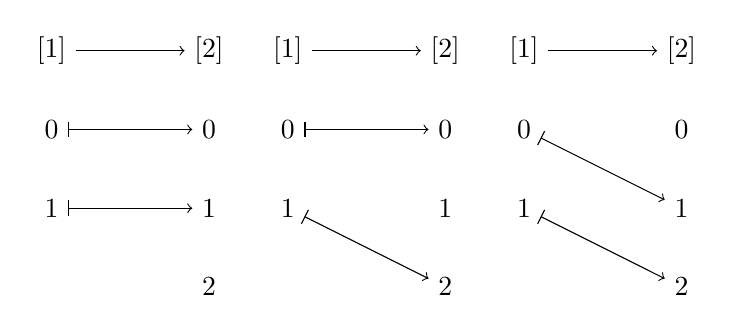
\begin{tikzpicture}
      \node (a1) at (0,3) {$[1]$}; \node (a2) at (2,3) {$[2]$};
      \node (b) at (0,2) {$0$}; \node (b') at (0,1) {$1$};
      \node (c) at (2,2) {$0$}; \node (d) at (2,1) {$1$}; \node (e) at (2,0) {$2$};
      \draw[|->] (b) to (c); \draw[|->] (b') to (d);
      \draw[->] (a1) to (a2);
      \node (b1) at (3,3) {$[1]$}; \node (b2) at (5,3) {$[2]$};
      \node (f) at (3,2) {$0$}; \node (f') at (3,1) {$1$}; 
      \node (g) at (5,2) {$0$}; \node (h) at (5,1) {$1$}; \node (i) at (5,0) {$2$};
      \draw[|->] (f) to (g); \draw[|->] (f') to (i);
      \draw[->] (b1) to (b2);
      \node (c1) at (6,3) {$[1]$}; \node (c2) at (8,3) {$[2]$};
      \node (j) at (6,2) {$0$}; \node (j') at (6,1) {$1$}; 
      \node (k) at (8,2) {$0$}; \node (l) at (8,1) {$1$}; \node (m) at (8,0) {$2$};
      \draw[|->] (j) to (l); \draw[|->] (j') to (m);
      \draw[->] (c1) to (c2);
    \end{tikzpicture}
  \end{center}
  である. 
  このとき, $\Delta^n_\calU$は$\del \Delta^n$と同一視できる. 
  \begin{center}
    \begin{tikzpicture}
      \node (a0) at (0,0) {$\{0\}$}; \node (a1) at (1.5,2.5) {$\{1\}$}; \node (a2) at (3,0) {$\{2\}$}; 
      \draw[->] (a0) to (a1); 
      \draw[->] (a1) to (a2); 
      \draw[->] (a0) to (a2); 
    \end{tikzpicture}
  \end{center}
\end{Proof}

\begin{example}
  $0 \leq i \leq n$とする. 
  $\calU$を$[n]$と$[n] \setminus \{i\}$を除いた(空でない)すべての部分集合の集まりとすると, $\Delta^n_\calU$は$\Lambda^n_i$に一致する.
\end{example}

\begin{exe}
  標準$n$単体$\Delta^n$の任意の単体的部分集合は$\Delta^n_\calU$の形であらわされる.
  このとき, $\calU$は$[n]$の(空でない)部分集合の下方で閉じている集まりで一意に決定されることを示せ. 
\end{exe}

\subsection{Kan複体}

$\Sing_\bullet$の形であらわされる単体的集合の特徴を調べる. 

\begin{definition}
  $\S$を単体的集合とする. 
  $\S$が次の条件
  \begin{itemize}
    \item[$(\ast)$] $n > 0$と$0 \leq i \leq n$に対して, すべての単体的集合の間の写像$\si_0: \Lambda^n_i \to \S$が拡張$\si: \Delta^n \to \S$をもつ. 
  \end{itemize}
  を満たすとき, $\S$をKan複体という. 
  \[\begin{tikzcd}
    {\Lambda^n_i} & {\S} \\
    {\Delta^n}
    \arrow["\si_0", from=1-1, to=1-2]
    \arrow[hook, from=1-1, to=2-1]
    \arrow["\si"', dashed, from=2-1, to=1-2]
  \end{tikzcd}\]
\end{definition}

\begin{exe}
  $n>0$のとき, 標準$n$単体$\Delta^n$はKan複体でない. (より一般の主張は命題1.2.4.2を参照)
\end{exe}

\begin{example}
  $\S$を次元$1$の単体的集合とする. 
  このとき, $\S$はKan複体でない. 
\end{example}

\begin{example}
  $\{S_{\al \bullet}\}_{\al \in A}$を集合$A$で添え字づけられた単体的集合の集まりとする. 
  $\S:=\prod_{\al \in A}S_{\al \bullet}$をそれらの直積とする. 
  各$S_{\al \bullet}$がKan複体であるとき, $\S$もKan複体である. 
  逆は各$S_{\al \bullet}$が空でない限り成立する. 
\end{example}

\begin{Proof}
  各$S_{\al \bullet}$はKan複体なので, $0 \leq i \leq n$に対して, 次の拡張が存在する. 
  \[\begin{tikzcd}
    {\Lambda^n_i} & {S_{\al \bullet}} \\
    {\Delta^n}
    \arrow["\si_{0,\al}", from=1-1, to=1-2]
    \arrow[hook, from=1-1, to=2-1]
    \arrow["\si_{\al}"', dashed, from=2-1, to=1-2]
  \end{tikzcd}\]
  直積の普遍性より, $\si_0: \Lambda^n_i \to S_{\al \bullet}$が一意に存在して次の図式が可換になる. 
  \[\begin{tikzcd}
    & {\Lambda^n_i} \\
    & {S_{\al \bullet}} \\
    {S_{\al1}} & \cdots
    \arrow["{\si_0}"', dashed, from=1-2, to=2-2]
    \arrow["{p_1}", from=2-2, to=3-1]
    \arrow["{\si_{0,1}}"', curve={height=12pt}, from=1-2, to=3-1]
  \end{tikzcd}\]
  同様に, $\si: \Delta^n \to S_{\al \bullet}$が一意に存在して次の図式が可換になる. 
  \[\begin{tikzcd}
    & {\Lambda^n_i} & {\Delta^n} \\
    & {S_{\al \bullet}} \\
    {S_{\al1}} & \cdots
    \arrow["{\si_0}"', dashed, from=1-2, to=2-2]
    \arrow["{p_1}", from=2-2, to=3-1]
    \arrow["{\si_{0,1}}"', curve={height=12pt}, from=1-2, to=3-1]
    \arrow[hook, from=1-2, to=1-3]
    \arrow["\si", dashed, from=1-3, to=2-2]
  \end{tikzcd}\]
  普遍性より, 右上の三角形は可換である. 
  \[\begin{tikzcd}
    {\Lambda^n_i} & {\S} \\
    {\Delta^n}
    \arrow["\si_0", from=1-1, to=1-2]
    \arrow[from=1-1, to=2-1]
    \arrow["\si"', dashed, from=2-1, to=1-2]
  \end{tikzcd}\]
  逆も直積の普遍性から示される. 
\end{Proof}

\begin{example}
  Kan複体の余直積
\end{example}

\begin{remark}
  例1.1.9.5と命題1.1.6.13より, $\S$がKan複体である必要十分条件は$\S$の各連結成分がKan複体であることである. 
\end{remark}

\begin{example}
  $S$を集合, $\uline{S}_\bullet$をその定数単体的集合とする.
  このとき, $\uline{S}_\bullet$はKan複体である. 
\end{example}

\begin{Proof}
  例1.1.6.10より, $\uline{S}_\bullet$の各連結成分は$\Delta^0$と同型である. 
  $\Delta^0$はKan複体なので, 注意1.1.9.6より$\uline{S}_\bullet$はKan複体である. 
\end{Proof}

\begin{prop}
  $X$を位相空間とする. 
  このとき, 特異単体的集合$\Sing_\bullet(X)$はKan複体である. 
\end{prop}

\begin{Proof}
  $\si_0: \Lambda^n_i \to \Sing_\bullet(X)$とする. 
  このとき, $\si_0$を$X$の標準$n$単体$\si: \Delta^n \to \Sing_\bullet(X)$に拡張できることを示せばよい. 
  幾何学的実現
  \footnote{
    幾何学的実現は特異単体関手の左随伴である. 
  }
  をもちいて$\si_0$を位相空間の間の連続写像$f_0: |\Lambda^n_i| \to X$とみなす. 
  この$f_0$を次のような合成
  \begin{align*}
    |\Lambda^n_i| \to |\Delta^n| \xr{f} X
  \end{align*}
  に分解したい. 
  \[\begin{tikzcd}
    {|\Lambda^n_i|} & {X} \\
    {|\Delta^n|}
    \arrow["{f_0}", from=1-1, to=1-2]
    \arrow["f"', dashed, from=2-1, to=1-2]
    \arrow[hook, from=1-1, to=2-1]
  \end{tikzcd}\]
  例1.1.8.13より, $|\Lambda^n_i|$は
  \begin{align*}
    |\Lambda^n_i| = \{(t_0,\cdots,t_n) \in |\Delta^n| : i\text{と異なるある}j \text{で} t_j=0\}
  \end{align*}
  とみなせる.
  よって, $r$を$|\Delta^n|$から$|\Lambda^n_i|$へのレクトクトとして, $f=f_0 \ci r$と分解できる. 
  \[\begin{tikzcd}
    {|\Lambda^n_i|} & {X} \\
    {|\Delta^n|}
    \arrow["{f_0}", from=1-1, to=1-2]
    \arrow["f"', dashed, from=2-1, to=1-2]
    \arrow[shift left=1, hook, from=1-1, to=2-1]
    \arrow["r", shift left=1, from=2-1, to=1-1]
  \end{tikzcd}\]
  例えば$r$を
  \begin{align*}
    r(t_0,\cdots,t_n) &:= (t_0-c,\cdots,t_{i-1}-c,t_i+nc,t_{i+1}-c,\cdots,t_n-c) \\
    c &:= \mathrm{min}\{t_0,\cdots,t_i,t_{i+1},\cdots,t_n\}
  \end{align*}
  とすればよい. 
  再び, 特異単体関手をもちいて
  \[\begin{tikzcd}
    {\Lambda^n_i} & {\Sing_\bullet(X)} \\
    {\Delta^n}
    \arrow["{\si_0}", from=1-1, to=1-2]
    \arrow["\si"', dashed, from=2-1, to=1-2]
    \arrow[hook, from=1-1, to=2-1]
  \end{tikzcd}\]
  を得る. 
\end{Proof}

\begin{prop}
  $G_\bullet$を単体的群(つまり, 群のなす圏の単体的対象)とする.
  このとき, $G_\bullet$(の台集合の単体的集合)はKan複体である. 
\end{prop}

$\S$を単体的集合とする. 
注意1.1.6.23より, 連結成分の集合$\pi_0(\S)$と写像$(d_0,d_1): S_1 \to S_0 \ti S_0$の像から生成される商集合$S_0 /{\sim}$を同一視できる. 
$\S=\Sing_\bullet(X)$の場合, 注意1.1.7.4より連結成分の集合は$\pi_0(\Sing_\bullet(X))=\pi_0(X)$である. 
また, 写像$(d_0,d_1): \Sing_1(X) \to \Sing_0(X) \ti \Sing_0(X) \simeq X \ti X$である. 
よって, $\S$が特異単体的集合の場合, $\pi_0(X)$と上の写像$(d_0,d_1)$の像を同一視できる. 
この議論は任意の単体的集合において言える.

\begin{prop}
  $\S$をKan複体, $x,y$を$\S$の点とする.
  $x$と$y$が同じ連結成分に属する必要十分条件は$d_0(e)=x, d_1(e)=y$を満たすある辺$e$が存在することである.  
\end{prop}

\begin{Proof}
  $R$を写像$(d_0,d_1): S_1 \to S_0 \ti S_0$の像とする.
  注意1.1.6.23より, $\pi_0(\S)$を$R$により生成される関係${\sim}$で割った商集合$S_0/{\sim}$と同一視する. 
  (執筆中)
\end{Proof}

\begin{cor}
  $\{S_{\al \bullet}\}$を集合$A$で添字づけられたKan複体の集まりとする.
  $\S:= \prod_{\al \in A} S_{\al \bullet}$をその直積とする. 
  このとき, 自然な射
  \begin{align*}
    \pi_0(\S) \to \prod_{\al \in A} \pi_0(S_{\al \bullet})
  \end{align*}
  は全単射である. 
  特に, $\S$が連結である必要十分条件は各$S_{\al \bullet}$が連結であることである. 
\end{cor}

\newpage

\section{圏のnerve}

1章では単体的集合の理論を説明して, 位相空間論との関係性を議論した. 
すべての位相空間$X$は単体的集合$\Sing_\bullet(X)$を定めて, $\Sing_\bullet(X)$の形であらわされる単体的集合はKan複体であるという特別な性質をもっていた. 
2章では圏論から生じる異なる単体的集合の種類について議論する. 
2章1節では圏$\calC$から定まる圏$\calC$のnerve
\footnote{
  nerveは脈体という和訳があるが, 本稿ではnerveと英語表記をする. 
}
と呼ばれる単体的集合$\N(\calC)$を定義する. 
2章2節では構成$\calC \mt \N(\calC)$が忠実充満であることを見る. 
2章3節では単体的集合$\S$が関手$\calC \mt \N(\calC)$の像の元である必要十分条件が, あるリフト条件を満たすことであることを示す. 
このリフト条件はKan拡張条件と類似している. 
2章4節では$\N(C)$の形であらわされる単体的集合がKan複体である必要十分条件が$\calC$における任意の射が可逆であることを示す. 

2章5節では構成$\calC \mt \N(\calC)$が左随伴をもち, 任意の単体的集合に対して, ホモトピー圏(homotopy category)と呼ばれる圏$\h \S$を定めることを見る. 
単体的集合$\S$が次元$\leq 1$であるとき, この圏は特別な書き方ができる. 
2章6節では, これが$\S$と一致する有向グラフ$G$のパスカテゴリー(path category)と同一視できることを示す. 

\subsection{nerveの構成}

\begin{cons}
  任意の$n$に対して, 線形順序集合$[n]$を通常の順序を入れることで圏とみなす. 
  圏$\calC$に対して, $[n]$から$\calC$へのすべての関手の集まりを$\mathrm{N}_n(\calC)$とあらわす. 
  任意の非減少写像$\al: [m] \to [n]$に対して, $\al$を前合成することで集合の間の写像$\mathrm{N}_n(\calC) \to \mathrm{N}_m(\calC)$が定まる. 
  この構成$[n] \mt \mathrm{N}_n(\calC)$は単体的集合とみなせる. 
  この単体的集合を$\N(\calC)$とあらわし, 圏$\calC$のnerveという. 
\end{cons}

\begin{remark}
  $\calC$を圏とする. 
  このとき, nerveの幾何学的実現$|\N(\calC)|$を圏$\calC$の分類空間(classifying space)という. 
  例1.2.4.3を参照. 
\end{remark}

\begin{remark}
  $C$を圏, $n \geq 1$とする. 
  $\mathrm{N}_n(\calC)$の元は圏$\calC$における図式
  \[\begin{tikzcd}
    {C_0} & {C_1} & \cdots & {C_n}
    \arrow[from=1-2, to=1-3]
    \arrow["{f_n}", from=1-3, to=1-4]
    \arrow["{f_1}", from=1-1, to=1-2]
  \end{tikzcd}\]
  とみなせる. 
  つまり, $\mathrm{N}_n(\calC)$の元は$0<i<n$に対して$f_{i+1}$の域と$f_i$の余域が等しい$\calC$における射の$n$組$(f_1,\cdots,f_n)$とみなせる. 
\end{remark}

\begin{example}
  $\calC$を圏とする. 
  このとき, 注意1.2.1.3より, 
  \begin{itemize}
    \item 単体的集合$\N(\calC)$の点は圏$\calC$の対象とみなせる. 
    \item 単体的集合$\N(\calC)$の辺は圏$\calC$の射とみなせる. 
    \item 圏$\calC$における射$f: X \to Y$を単体的集合$\N(\calC)$の辺とみなす. 
    このとき, $f$の面は余域が$d_0f=Y$, 域が$d_1f=X$で与えられる.
    \item $\calC$の対象$X$を単体的集合$\N(\calC)$の点とみなす. 
    このとき, 退化な辺$s_0(X)$は恒等射$\id_X: X \to X$である. 
  \end{itemize}
\end{example}

より一般に, 次の関係が成立する. 

\begin{remark}
  $\calC$を圏 ,$n>0$とする. 
  単体的集合$\N(\calC)$の$n$単体$\si$を図式
  \[\begin{tikzcd}
    {C_0} & {C_1} & \cdots & {C_n}
    \arrow[from=1-2, to=1-3]
    \arrow["{f_n}", from=1-3, to=1-4]
    \arrow["{f_1}", from=1-1, to=1-2]
  \end{tikzcd}\]
  とみなす. 
  このとき, 
  \begin{itemize}
    \item $0$番目の面写像$d_0\si \in \mathrm{N}_{n-1}(\calC)$は対象$C_0$と域を$C_0$にもつ射$f_1$を「消去」した図式
    \[\begin{tikzcd}
      {C_1} & {C_2} & \cdots & {C_n}
      \arrow[from=1-2, to=1-3]
      \arrow["{f_n}", from=1-3, to=1-4]
      \arrow["{f_2}", from=1-1, to=1-2]
    \end{tikzcd}\]
    とみなせる. 
    \item $n$番目の面写像$d_n\si \in \mathrm{N}_{n-1}(\calC)$は対象$C_n$と余域を$C_n$にもつ射$f_n$を「消去」した図式
    \[\begin{tikzcd}
      {C_0} & {C_1} & \cdots & {C_{n-1}}
      \arrow[from=1-2, to=1-3]
      \arrow["{f_{n-1}}", from=1-3, to=1-4]
      \arrow["{f_1}", from=1-1, to=1-2]
    \end{tikzcd}\]
    とみなせる. 
    \item $0<i<n$に対して, $i$番目の面写像$d_n\si \in \mathrm{N}_{n-1}(\calC)$は$C_i$を「消去」して射$f_i$と$f_{i+1}$を合成した図式
    \[\begin{tikzcd}
      {C_0} & {C_1} & \cdots & {C_{i-1}} & {C_{i+1}} & \cdots & {C_n}
      \arrow["{f_{i+1} \ci f_i}", from=1-4, to=1-5]
      \arrow[from=1-5, to=1-6]
      \arrow["{f_n}", from=1-6, to=1-7]
      \arrow[from=1-3, to=1-4]
      \arrow["{f_1}", from=1-1, to=1-2]
      \arrow[from=1-2, to=1-3]
    \end{tikzcd}\]
    とみなせる. 
  \end{itemize}
\end{remark}

\begin{remark}
  $\calC$を圏 ,$n>0$とする. 
  単体的集合$\N(\calC)$の$n$単体$\si$を図式
  \[\begin{tikzcd}
    {C_0} & {C_1} & \cdots & {C_n}
    \arrow[from=1-2, to=1-3]
    \arrow["{f_n}", from=1-3, to=1-4]
    \arrow["{f_1}", from=1-1, to=1-2]
  \end{tikzcd}\]
  とみなす. 
  このとき, $0 \leq i \leq n$に対して, $s_i\si \in \mathrm{N}_{n+1}(\calC)$は恒等射$\id_{C_i}$を「挿入」した図式
  \[\begin{tikzcd}
    {C_0} & \cdots & {C_{i-1}} & {C_i} & {C_i} & {C_{i+1}} & \cdots & {C_n}
    \arrow["{f_{i+1}}", from=1-5, to=1-6]
    \arrow[from=1-6, to=1-7]
    \arrow["{f_n}", from=1-7, to=1-8]
    \arrow["{\id_{C_i}}", from=1-4, to=1-5]
    \arrow["{f_{i-1}}", from=1-2, to=1-3]
    \arrow["{f_i}", from=1-3, to=1-4]
    \arrow["{f_1}", from=1-1, to=1-2]
  \end{tikzcd}\]
  とみなせる. 
\end{remark}

\begin{remark}
  $\calC$を圏 ,$n>0$とする. 
  単体的集合$\N(\calC)$の$n$単体$\si$を図式
  \[\begin{tikzcd}
    {C_0} & {C_1} & \cdots & {C_n}
    \arrow[from=1-2, to=1-3]
    \arrow["{f_n}", from=1-3, to=1-4]
    \arrow["{f_1}", from=1-1, to=1-2]
  \end{tikzcd}\]
  とみなす. 
  このとき, $\si$が退化である必要十分条件はある$i$で$f_i$が$\calC$における恒等射であることである. 
\end{remark}

\begin{remark}
  半順序$\leq_I$を備えた集合$I$を圏とみなし, この半順序集合のnerveを$\N(I)$とあらわす. 
  $\N(I)$の$n$単体は単調写像$[n] \to I$, つまり$I$の非減少な列$(i_0 \leq_I \cdots \leq_I i_n)$とみなせる. 
\end{remark}

\begin{example}
  nerve $\N([n])$は標準$n$単体$\Delta^n$とみなせる. 
\end{example}

\begin{Proof}
  $\N([n])$の$m$-単体が$\mathrm{N}([n])_m=\Hom([m],[n])$であることから分かる. 
\end{Proof}

\begin{remark}
  構成$\calC \mt \N(\calC)$は小圏のなす圏から単体的集合のなす圏への関手$\N: \cat \to \sset$を定める. 
  この関手をnerve関手(nerve functor)という. 
  これは定義1.1.7.7の例である. 
  実際, $Q:\csim \to \cat$を線形順序集合$[n] \in \csim$を圏とみなす関手と思うと, $\N$は関手$\Sing_\bullet^Q: \cat \to \sset$と思える. 
  命題1.1.8.22より, nerve関手は左随伴をもつ. (2章5節を参照)
\end{remark}

\subsection{nerveからの圏の復元}

nerve関手$\cat \to \sset: \calC \mt \N(\calC)$は情報を失わない. 

\begin{prop}
  nerve関手$\N: \cat \to \sset$は忠実充満である. 
\end{prop}

\begin{Proof}
  
\end{Proof}

nerve関手が忠実充満であるので, 圏$\calC$とそのnerve $\N(\calC)$を同一視する. 
これより, 圏はある特別な単体的集合と思える. 

\subsection{nerveの特徴づけ}

nerve関手$\N: \cat \to \sset$の像について調べる. 

\begin{prop}
  $\S$を単体的集合とする. 
  このとき, $\S$がある圏$\calC$のnerveである必要十分条件は次の条件
  \begin{itemize}
    \item[$(\ast')$] $0<i<n$に対して, 単体的集合の間の写像$\si: \Lambda^n_i \to \S$が一意な拡張$\si: \Delta^n \to \S$をもつ.
  \end{itemize} 
  を満たすことである. 
\end{prop}

まずは必要条件を示す. 

\begin{lemma}
  $\calC$を圏とする. 
  このとき, 単体的集合$\N(\calC)$は条件$(\ast')$を満たす. 
\end{lemma}

\begin{lemma}
  $f: \S \to \T$を単体的集合の間の写像とする. 
  $f$が同型$S_0 \to T_0, S_1 \to T_1$を誘導して, $\S, \T$が条件$(\ast')$を満たすとき, $f$は同型射である. 
\end{lemma}

これで命題1.2.3.1を示す準備が整った. 

\begin{Proof}
  必要条件はすでに示したので, 十分条件を示す. 
\end{Proof}

\begin{remark}
  命題1.2.3.1の条件$(\ast)$と同値な条件は多く存在する. 
  例えば, priori弱条件(priori weaker condition)と呼ばれる次の条件
  \begin{itemize}
    \item[$(\ast_0')$] $n \geq 2$に対して, すべての単体的集合の間の写像$\si_0: \Lambda^n_1 \to \S$が一意な拡張$\Delta^n \to \S$をもつ.
  \end{itemize}
  に変えてもよい. 
\end{remark}

\subsection{亜群のnerve}

命題1.2.2.1より, nerve $\N(\calC)$から圏同値の違いをのぞいて圏$\calC$を復元することができる. 
特に, 圏$\calC$上において圏同値で不変な条件は単体的集合$\N(\calC)$上の条件として定式化することができる. 
これを簡単な例で見る. 

\begin{definition}
  圏$\calC$の任意の射が可逆であるとき, $\calC$を亜群(groupoid)という. 
\end{definition}

\begin{prop}
  $\calC$を圏とする. 
  $\calC$が亜群である必要十分条件は単体的集合$\N(\calC)$がKan複体であることである. 
\end{prop}

\begin{Proof}
  十分条件を示す. 
  $\N(\calC)$がKan複体であるとする. 
  $f: C \to D$を$\calC$における射とする. 
  写像$\Hom_{\sset}(\Delta^2,\N(\calC)) \to \Hom_{\sset}(\Lambda^2_2,\N(\calC))$の全射性
  \footnote{
    Kan複体の拡張条件において, $n=2,i=2$としたものである. 
  }
  より, $d_0(\si)=f, d_1(\si)=\id_D$を満たす$\N(\calC)$のある$2$単体$\si$が存在する. 
  \begin{center}
    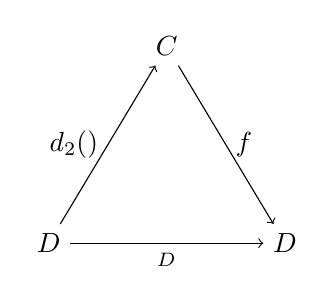
\begin{tikzpicture}
      \node (a1) at (0,0) {$D$}; \node (a2) at (3,0) {$D$}; \node (a3) at (1.5,2.5) {$C$}; 
      \node (c1) at (1.5,1.0) {$\si$};
      \draw[->] (a1) to node[left] {$d_2(\si)$} (a3); 
      \draw[->] (a3) to node[right] {$f$} (a2); 
      \draw[->] (a1) to node[below] {$\id_D$} (a2); 
    \end{tikzpicture}
  \end{center}
  $g:=d_2(\si)$とすれば, $f \ci g=\id_D$を得る. 
  同様に, $\Hom_{\sset}(\Delta^2,\N(\calC)) \to \Hom_{\sset}(\Lambda^2_0,\N(\calC))$の全射性より, 
  \begin{center}
    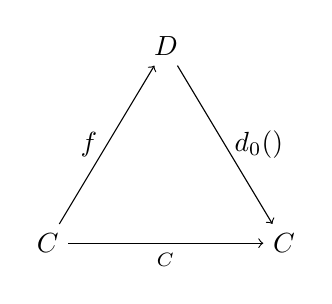
\begin{tikzpicture}
      \node (a1) at (0,0) {$C$}; \node (a2) at (3,0) {$C$}; \node (a3) at (1.5,2.5) {$D$}; 
      \node (c1) at (1.5,1.0) {$\si$};
      \draw[->] (a1) to node[left] {$f$} (a3); 
      \draw[->] (a3) to node[right] {$d_0(\si)$} (a2); 
      \draw[->] (a1) to node[below] {$\id_C$} (a2); 
    \end{tikzpicture}
  \end{center}
  $h:=d_0(\si)$とすれば, $h \ci f=\id_C$を得る. 
  \begin{align*}
    g = \id_C \ci g = (h \ci f) \ci g = h \ci (f \ci g) = h \ci \id_D = h
  \end{align*}
  よって, $f \ci g=\id_D, g \ci f=\id_C$なので$g$は$f$の逆射である. \\
  必要条件を示す. 
  圏$\calC$が亜群であるとする. 
  補題1.2.3.2より, $0<i<n$に対して$\Lambda^n_i \to \N(\calC)$は拡張$\Delta^n \to \N(\calC)$をもつ. 
  (これは圏が亜群であることは必要でない.)
  よって, 後は$i=0,n$の場合を考えればよい. 
\end{Proof}

\begin{example}
  $M$をモノイドとする. 
  このとき, 圏$BM$を次のように構成する. 
  \begin{itemize}
    \item 対象は$M$のある1つの対象$X$
    \item $\Hom_{BM}(X,X):=M$
    \item 合成は$M$の乗法
  \end{itemize}
  この圏$BM$のnerveを$\B M$とあらわす. 

  特にモノイド$M$が群$G$である場合, 幾何学的実現$|\B G|$は$G$の分類空間(classifying space)と呼ばれる位相空間である. 
  これは分類空間が次のいずれかの性質をもつCW複体であることから, ホモトピー同値の違いをのぞいて一意に決定される. 
  \begin{itemize}
    \item 位相空間$|\B G|$は連結で, そのホモトピー群はそれぞれの基点に対して
    \begin{align*}
      \pi_\ast (|\B G|) \simeq 
      \begin{cases}
        G &(\ast=1) \\
        0 &(\ast >1)
      \end{cases}
    \end{align*}
    である. 
    \footnote{
      $n$-連結などを参照
    }
    \item 任意のパラコンパクトな位相空間$X$に対して, 自然な全単射
    \begin{align*}
      \{\text{連続写像}f: X \to |\B G|\}/\text{ホモトピー} 
      \simeq \{\text{G-tosor}: P \to X\}/\text{同型射}
    \end{align*}
    が存在する. 
  \end{itemize}
  詳しい議論は\cite{MJ3}を参照. 
\end{example}

この節の最後に圏と亜群との関係を述べる. 

\begin{cons}
  $\calC$を圏とする. 
  部分圏$\calC^\simeq \subset \calC$を次のように定義する. 
  \begin{itemize}
    \item $\calC^\simeq$の対象は$\calC$の対象 
    \item $\calC^\simeq$の射は$\calC$における同型射 
  \end{itemize}
  $\calC^\simeq$を$\calC$の中心(core)という. 
\end{cons}

\begin{remark}
  $\calC$を圏とする. 
  中心 $\calC^\simeq$は次の性質から, 圏同値の違いをのぞいて一意に決定される. 
  \begin{itemize}
    \item 圏$\calC^\simeq$は亜群である. 
    \item $\calD$が亜群のとき, 任意の関手$F: \calD \to \calC$は$\calC^\simeq$を経由して一意に分解される. 
    \[\begin{tikzcd}
      \calD & {\calC^\simeq} & \calC
      \arrow[from=1-1, to=1-2]
      \arrow[from=1-2, to=1-3]
    \end{tikzcd}\]
  \end{itemize}
\end{remark}

\subsection{単体的集合のホモトピー圏}

nerve関手$\N: \cat \to \sset: \calC \mt \N(\calC)$が左随伴をもつことを示す. 

\begin{definition}
  $\calC$を圏とする. 
  任意の圏$\calD$に対して, 合成
  \begin{align*}
    \Hom_{\cat}(\calC,\calD) \to \Hom_{\sset}(\N(\calC),\N(\calD)) 
    \xr{- \ci u} \Hom_{\sset}(\S,\N(\calD)) 
  \end{align*}
  が全単射であるとき, 単体的集合の間の写像$u: \S \to \N(\calC)$は$\S$のホモトピー圏として$\calC$を示す($u$ exhibits $\calC$ as the homotopy category of $\S$)という. 
  (命題1.2.2.1より左側は常に全単射である.) 
\end{definition}

\begin{exe}
  
\end{exe}

\begin{remark}
  $\S$を単体的集合とする. 
  ある圏$\calC$と$\S$のホモトピー圏として$\calC$を示す写像$\S \to \N(\calC)$が存在するとする. 
  このとき, 圏$\calC$は同型の違いをのぞいて一意に決定される. 
  これは$\S$の関手性による. 
  よって, $\calC$を$\S$のホモトピー圏といい, $\h \S$とあらわす. 
\end{remark}

\begin{prop}
  $\S$を単体的集合とする. 
  このとき, ある圏$\calC$と$\S$のホモトピー圏として$\calC$を示す単体的集合の間の写像$\S \to \N(\calC)$が存在する.
\end{prop}

\begin{Proof}
  
\end{Proof}

\begin{cor}
  nerve関手$\N: \cat \to \sset$は構成$\S \mt \h \S$による左随伴をもつ. 
\end{cor}

\begin{Proof}
  命題1.2.5.4より
  \begin{align*}
    \Hom_{\cat}(\h \S,\calD) \simeq \Hom_{\sset}(\S,\N(\calD)) 
  \end{align*}
  が存在することから分かる. 
\end{Proof}

\begin{remark}
  $\calC$を圏とする. 
  随伴$\h \dav \N$の余単位は圏同値$\h \N(\calC) \simeq \calC$を誘導する. 
  これは命題1.2.2.1の言い換えである. 
  つまり, 任意の圏$\calC$はnerve $\N(\calC)$のホモトピー圏として復元できる. 
\end{remark}

\begin{remark}
  
\end{remark}

\subsection{例: 有向グラフのパスカテゴリー}

\newpage

\section{\texorpdfstring{$\infty$}{infty}-圏}

1章と2章で単体的集合$\S$について2つの条件
\begin{itemize}
  \item[$(\ast)$] $n>0$と$0 \leq i \leq n$に対して, 任意の射$\si_0: \Lambda^n_i \to \S$が拡張$\si: \Delta^n \to \S$をもつ.
  \item[$(\ast')$] $0<i<n$に対して, 任意の射$\si_0: \Lambda^n_i \to \S$が一意な拡張$\si: \Delta^n \to \S$をもつ. 
\end{itemize}
を考えた. 

条件$(\ast)$を満たす単体的集合はKan複体と呼ばれ, ホモトピー論への組み合わせ論的な方法を与えるものであった.
条件$(\ast')$を満たす単体的集合は圏(のnerve)とみなされた.(命題1.2.2.1と命題1.2.3.1)
この2つの条件から共通の一般化が考えられる. 

\begin{definition}
  $\infty$-圏($\infty$-category)とは次の条件
  \begin{itemize}
    \item[$(\ast'')$] $0<i<n$に対して, 任意の射$\si_0: \Lambda^n_i \to \S$が拡張$\si: \Delta^n \to \S$をもつ.
  \end{itemize}
  を満たす単体的集合である. 
\end{definition}

\begin{remark}
  条件$(\ast'')$は弱Kan拡張条件(weak Kan extention condition)と呼ばれる. 
  BoardmanとVogtにより導入された概念であり, 彼らはこの$\infty$-圏を弱Kan複体(weak Kan complex)と呼んだ. 
  この理論はJoyalにより更に発展し, この$\infty$-圏を擬圏(quasi-category)と呼んだ. 
\end{remark}

\begin{example}
  任意のKan複体は$\infty$-圏である. 
  特に, 位相空間$X$に対して特異単体的集合$\Sing_\bullet(X)$はKan複体であるので, $\infty$-圏である.
\end{example}

\begin{example}
  任意の圏$\calC$に対して, nerve $\N(\calC)$は$\infty$-圏である. 
\end{example}

\begin{remark}
  nerve関手が忠実充満な埋め込みであったので, 圏$\calC$とそのnerve $\N(\calC)$は同一視できる.
  これより, 例1.3.0.3は「任意の圏は$\infty$-圏である」ということができる. 
  以降では, 混乱しないために, 圏を通常の圏(ordinary category)ということにする. 
\end{remark}

\begin{example}
  $\{S_{\al \bullet}\}_{\al \in A}$を集合$A$で添え字づけられた単体的集合の集まりとする. 
  $\S:=\prod_{\al \in A}S_{\al \bullet}$をそれらの直積とする. 
  各$S_{\al \bullet}$が$\infty$-圏であるとき, $\S$も$\infty$-圏である. 
  逆は各$S_{\al \bullet}$が空でない限り成立する. 
\end{example}

\begin{Proof}
  例1.1.9.4と同様
\end{Proof}

\begin{example}
  無限圏の余直積
\end{example}

\begin{Proof}
  例1.1.9.5と同様
\end{Proof}

\begin{remark}
  $\S$を単体的集合とする. 
  例1.3.0.7と命題1.1.6.13より, $\S$が$\infty$-圏である必要十分条件は$\S$の連結成分がそれぞれ$\infty$-圏であることである. 
\end{remark}

\begin{remark}
  $\{S(\al)_\bullet\}$を余極限$\S:=\varinjlim S(\al)_\bullet$をもつフィルターつき図式とする.
  各$S(\al)_\bullet$が$\infty$-圏であるとき, $\S$は$\infty$-圏である. 
\end{remark}

通常の圏のように, $\infty$-圏を$\calC$や$\calD$であらわし, 通常の圏の言葉を用いる. 
例えば, $\calC=\S$を$\infty$-圏とするとき, 単体的集合$\S$の点を$\infty$-圏の対象, 単体的集合$\S$の辺を$\infty$-圏の射とみなす. (3章1節)
本稿の目的は$\infty$-圏が圏のようにふるまうことを示すことである. 
特に, 任意の$\infty$-圏に対して$\calC$の射の合成が考えられることをみる. (3章4節)
$\calC$の射$f: X \to Y$と$g: Y \to Z$の組, つまり$d_0(f)=d_1(g)$を満たす$S_1$の辺$f,g$は単体的集合の間の写像$\si_0: \Lambda^2_1 \to \calC$を定める. 
\begin{center}
  \begin{tikzpicture}
    \node (a0) at (0,0) {$X$}; \node (a1) at (1.5,2.5) {$Y$}; \node (a2) at (3,0) {$Z$};  
    \node (c1) at (1.5,1.0) {$\si$};
    \draw[->] (a0) to node[left] {$f$} (a1); 
    \draw[->] (a1) to node[right] {$g$} (a2); 
  \end{tikzpicture}
\end{center}
条件$(\ast'')$より, $\si_0$を$\calC$の$2$単体$\si$に拡張することができる. 
\begin{center}
  \begin{tikzpicture}
    \node (a0) at (0,0) {$X$}; \node (a1) at (1.5,2.5) {$Y$}; \node (a2) at (3,0) {$Z$};  
    \node (c1) at (1.5,1.0) {$\si$};
    \draw[->] (a0) to node[left] {$f$} (a1); 
    \draw[->] (a1) to node[right] {$g$} (a2); 
    \draw[->] (a0) to node[below] {$d_1(\si)$} (a2); 
  \end{tikzpicture}
\end{center}
このとき, 射$h:=d_1(\si)$を$f$と$g$の合成とみなす. 
この合成$\si$は一意ではないので, $h$は$f$と$g$のみでは完全には定まらない.
しかし, これはあるホモトピー(homotopy)の違いをのぞいて一意に決定される. (3章5節)
これを用いて, $\calC$が$\infty$-圏であるときのホモトピー圏$\h \calC$を具体的に書き下すことができる.

\subsection{\texorpdfstring{$\infty$}{infty}-圏における対象と射}

\begin{definition}
  $\calC=\S$を$\infty$-圏とする. 
  単体的集合$\S$の点, つまり集合$S_0$の元を$\calC$の対象(object)という. 
  単体的集合$\S$の辺, つまり集合$S_1$の元を$\calC$の射(morphism)という. 
  $f \in S_1$を$\calC$の射とするとき, 対象$X:=d_1(f)$を$f$の域(source), 対象$Y:=d_0(f)$を$f$の余域(target)という. 
  このとき, $f$を$X$から$Y$への射という. 
  任意の対象$X$に対して, 退化な辺$s_0(X)$は$X$から$X$への辺とみなせる. 
  この射を$\id_X$とあらわし, $X$の恒等射(identity morphism)という. 
  \footnote{
    合成は3章4節で定義する. 
  }
\end{definition}

\begin{nota}
  $\calC$を$\infty$-圏とする. 
  $X$が$\calC$の対象であるとき, $X \in \calC$とあらわす. 
  $f$が$X$から$Y$への射であるとき, 「$f: X \to Y$は$\calC$の射である」という. 
\end{nota}

\begin{example}
  $\calC$を通常の圏として, 単体的集合$\N(\calC)$を$\infty$-圏とみなす. 
  このとき, 例1.2.1.4より
  \begin{itemize}
    \item $\infty$-圏$\N(\calC)$の対象は$\calC$の対象
    \item $\infty$-圏$\N(\calC)$の射は$\calC$の射である. 
    更に, $\calC$における射の域と余域は$\N(\calC)$における射の域と余域に等しい.
    \item 任意の対象$X \in \calC$に対して, 恒等射$\id_x$は$X$を通常の圏$\calC$の対象とみなしても, $\infty$-圏$\N(\calC)$の対象とみなしても同じである. 
  \end{itemize}
\end{example}

\begin{example}
  $X$を位相空間として, $\Sing_\bullet(X)$を$\infty$-圏とみなす. 
  このとき, 例1.1.7.2より
  \begin{itemize}
    \item $\infty$-圏$\Sing_\bullet(X)$の対象は$X$の点 
    \item $\infty$-圏$\Sing_\bullet(X)$の射は連続な道$f: [0,1] \to X$である. 
    射$f$の域と余域はそれぞれ位相空間$X$の点$f(0), f(1)$である. 
    \item 任意の点$x \in X$に対して, 恒等射$\id_x$は$x$に値をとる定値な道$[0,1] \to X$
  \end{itemize}
\end{example}

\subsection{反転\texorpdfstring{$\infty$}{infty}-圏}

通常の圏$\calC$に対して, 反転圏(oposite category) $\calC^\OP$を考えることができる. 
構成$\calC \mt \calC^\OP$を$\infty$-圏においても考える. 
実際, この構成は任意の単体的集合に対して考えることができる. 

\begin{nota}
  対象が有限線形順序集合で, 射が非減少な関数であるような圏を$\Lin$とあらわす. 
  $Lin$の対象$I$を線形順序$\leq_I$が備わった集合とみなす. 
  同じ台集合で, 反転した順序$\leq_{I^\OP}$をもつ線形順序集合を$I^\OP$とあらわす. 
  つまり, 次の関係が成立する. 
  \begin{align*}
    i \leq_{I^\OP} j \Leftrightarrow j \leq_I i
  \end{align*}
  構成$I \mt I^\OP$は$\Lin$から$\Lin$への圏同値を定める. 
\end{nota}

単体圏$\csim$は$[n]=\{0 < \cdots < n\}$の形であらわされる対象で張られる$\Lin$の充満部分圏である. 
また, 次の図式
\[\begin{tikzcd}
	\csim & \Lin \\
	\csim & \Lin
	\arrow["\Op"', from=1-1, to=2-1]
	\arrow[hook, from=1-1, to=1-2]
	\arrow["{I \mt I^\OP}", from=1-2, to=2-2]
	\arrow[hook, from=2-1, to=2-2]
\end{tikzcd}\]
を同型の違いをのぞいて可換にする一意な関手$\Op: \csim \to \csim$が存在する. 
関手$\Op$は次のように書き下すことができる. 
\begin{itemize}
  \item $[n] \in \csim$に対して, $i \mt n-i$によって$[n]$から反転した順序の入った$[n]^\OP$への同型射で与えられる. 
  \item $\al: [m] \to [n]$に対して, $\Op(\al): [m] \to [n]: i \mt n-\al(m-i)$で与えられる.  
\end{itemize}

\begin{cons}
  $\S: \simop \to \cset$を単体的集合とする. 
  このとき, 単体的集合$\S^\OP$を次のような合成
  \begin{align*}
    \simop \xr{\Op} \simop \xr{\S} \cset
  \end{align*}
  と定義する. 
  この$\S^\OP$を単体的集合$\S$の反転単体的集合(opposite of the simplicial set)という.
\end{cons}

\begin{remark}
  $\S$を単体的集合とする. 
  反転単体的集合$\S^\OP$は$\Op$の定義から次のように書き下すことができる. 
  \begin{itemize}
    \item 各$n$に対して, $S^\OP_n=S_n$
    \item $\S^\OP$の面写像と退化写像は次で与えられる. 
    \begin{align*}
      d_i: S^\OP_n \to S^\OP_{n-1} &= d_{n-i}: S_n \to S_{n-1} \\
      s_i: S^\OP_n \to S^\OP_{n+1} &= s_{n-i}: S_n \to S_{n+1} 
    \end{align*}
  \end{itemize}
\end{remark}

\begin{example}
  $\calC$を通常の圏とする. 
  $\N (\calC)$の$n$単体$\si$を圏$\calC$における次の図式
  \[\begin{tikzcd}
    {C_0} & {C_1} & \cdots & {C_n}
    \arrow[from=1-2, to=1-3]
    \arrow["{f_n}", from=1-3, to=1-4]
    \arrow["{f_1}", from=1-1, to=1-2]
  \end{tikzcd}\]
  とみなす. 
  このとき, $\si$は$\N (\calC^\OP)$の$n$単体$\si'$を$\calC^\OP$における次の図式
  \[\begin{tikzcd}
    {C_n} & {C_{n-1}} & \cdots & {C_0}
    \arrow[from=1-2, to=1-3]
    \arrow["{f_1}", from=1-3, to=1-4]
    \arrow["{f_n}", from=1-1, to=1-2]
  \end{tikzcd}\]
  として定める. 
  構成$\si \mt \si'$は単体的集合の間の同型$\N(\calC)^\OP \simeq \N(\calC^\OP)$を定める. 
\end{example}

\begin{example}
  $X$を位相空間とする. 
  同型写像$r: |\Delta^n| \to |\Delta^n|: (t_0,\cdots,t_n) \mt (t_n,\cdots,t_0)$を用いて, 
  $\Sing_\bullet(X)$の$n$単体$\si: |\Delta^n| \to X$を合成
  \begin{align*}
    |\Delta^n| \xr{r} |\Delta^n| \xr{\si} X
  \end{align*}
  に送る. 
  これにより, 自然な同型$\Sing_\bullet(X) \simeq \Sing^{\OP}_{\bullet}$が定まる. 
\end{example}

\begin{prop}
  $\calC$を$\infty$-圏とする. 
  このとき, 反転単体的集合$\calC^\OP$も$\infty$-圏である. 
\end{prop}

\begin{Proof}
  $0<i<n$に対して, $\si_0: \Lambda^n_i \to \calC^\OP$が$\si: \Delta^n \to \calC^\OP$に拡張できることを見る. 
  関手$\Op$が圏同値であることから, $\si_0^\OP: (\Lambda^n_i)^\OP \to \calC$が$\si^\OP: (\Delta^n)^\OP \to \calC$に拡張できることを見ればよい. 
  関手$\Op$の構成より, 自然な同型$(\Delta^n)^\OP \simeq \Delta^n$が存在して, $(\Lambda^n_i)^\OP$を$\Lambda^n_{n-i}$に送る. 
  $\calC$は$\infty$-圏であるので, $\Lambda^n_{n-i} \to \calC$を$\Delta^n \to \calC$に拡張することができる. 
\end{Proof}

\begin{remark}
  $\calC$を$\infty$-圏とする. 
  $\infty$-圏$\calC^\OP$を$\infty$-圏の反転$\infty$-圏(opposite of the $\infty$-category)という. 
  \begin{itemize}
    \item $\calC^\OP$の対象は$\calC$の対象
    \item $X,Y \in \calC$に対して, $\calC^\OP$における$X$から$Y$への射は$\calC$における$Y$から$X$への射 
  \end{itemize}
\end{remark}

\subsection{\texorpdfstring{$\infty$}{infty}-圏における射のホモトピー}

任意の位相空間$X$に対して, 特異単体的集合$\Sing_\bullet(X)$は$\infty$-圏である. 
$\infty$-圏$\Sing_\bullet(X)$において, 点$x \in X$から点$y \in X$への射は$f(0)=x,f(1)=y$を満たす連続な道$f: [0,1] \to X$である. 
多くの目的のために, (例えば, 基本亜群$\pi_1(X,x)$を調べるように)道ではなく端点を固定した道のホモトピー類(homotopy class)を考えることは有用である. 
この考えを任意の$\infty$-圏に一般化する. 

\begin{definition}
  $\calC$を$\infty$-圏とする. 
  $f,g: X \to Y$を同じ域と余域をもつ射とする. 
  $f$から$g$へのホモトピー(homotopy)とは$d_0(\si)=\id_Y, d_1(\si)=g, d_2(\si)=f$を満たす$\calC$の$2$単体$\si$である. 
  \begin{center}
    \begin{tikzpicture}
      \node (a0) at (0,0) {$X$}; \node (a2) at (3,0) {$Y$}; \node (a1) at (1.5,2.5) {$Y$}; 
      \node (c1) at (1.5,1.0) {$\si$};
      \draw[->] (a0) to node[left] {$f$} (a1); 
      \draw[->] (a1) to node[right] {$\id_Y$} (a2); 
      \draw[->] (a0) to node[below] {$g$} (a2); 
    \end{tikzpicture}
  \end{center}
  $f$から$g$へのホモトピーが存在するとき, $f$と$g$はホモトピック(homotopic)であるという. 
\end{definition}

\begin{example}
  $\calC$を通常の圏とする. 
  $\calC$における射$f,g: C \to D$が$\infty$-圏$\N(\calC)$における射としてホモトピックである必要十分条件は$f=g$である. 
\end{example}

\begin{example}
  $X$を位相空間, $x,y$を$X$の点とする. 
  $f(0)=g(0)=x$と$f(1)=g(1)=y$を満たす連続な道$f,g: [0,1] \to X$が$\infty$-圏$\Sing_\bullet(X)$における射としてホモトピックである必要十分条件は通常の意味で$f$と$g$がホモトピックであることである. 
\end{example}

\begin{exe}
  
\end{exe}

\begin{prop}
  $X,Y$を$\infty$-圏$\calC$の対象とし, $E$を$\calC$における$X$から$Y$へのすべての射の集まりとする.
  ホモトピーは$E$における同値関係である. 
  ホモトピーによる同値類をホモトピー類という. 
\end{prop}

\begin{Proof}
  反射律を示す. 
  任意の射$f: X \to Y$に対して, $2$単体$s_1(f)$は$f$から$f$へのホモトピーである. 
  \begin{center}
    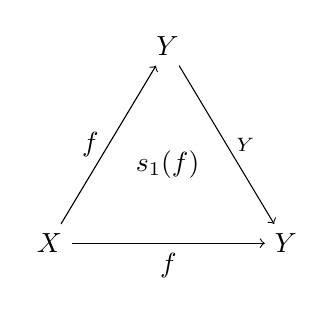
\begin{tikzpicture}
      \node (a0) at (0,0) {$X$}; \node (a2) at (3,0) {$Y$}; \node (a1) at (1.5,2.5) {$Y$}; 
      \node (c1) at (1.5,1.0) {$s_1(f)$};
      \draw[->] (a0) to node[left] {$f$} (a1); 
      \draw[->] (a1) to node[right] {$\id_Y$} (a2); 
      \draw[->] (a0) to node[below] {$f$} (a2); 
    \end{tikzpicture}
  \end{center}
  対称律と推移律を示すために次の命題を考える. 
  \begin{itemize}
    \item[$(\ast)$] $f,g,h$を$X$から$Y$への射とする. 
    $f$と$g$がホモトピックで$f$と$h$がホモトピックであるとき, $g$と$h$はホモトピックである. 
  \end{itemize}
  $h=f$の場合, 「$f$と$g$がホモトピックで$f$と$f$がホモトピックであるとき, $g$と$f$はホモトピックである」となる. 
  反射律を用いると, これは対称律であることを示している. 
  $f$と$g$を入れ替えると, 「$g$と$f$がホモトピックで$g$と$h$がホモトピックであるとき, $f$と$h$はホモトピックである」となる. 
  対称律を用いると, これは推移律であることを示している. 
  よって, 命題$(\ast)$を示せば十分である. 
  $f$と$h$, $f$と$g$, $\id_Y$がホモトピックであることをそれぞれ次のようにあらわす. 
  \begin{center}
    \begin{tikzpicture}
      \node (a1) at (0,0) {$X$}; \node (a2) at (3,0) {$Y$}; \node (a3) at (1.5,2.5) {$Y$}; 
      \node (c1) at (1.5,1.0) {$\si_2$};
      \draw[->] (a1) to node[left] {$f$} (a3); 
      \draw[->] (a3) to node[right] {$\id_Y$} (a2); 
      \draw[->] (a1) to node[below] {$h$} (a2); 
      \node (b1) at (4,0) {$X$}; \node (b2) at (7,0) {$Y$}; \node (b3) at (5.5,2.5) {$Y$}; 
      \node (c2) at (5.5,1.0) {$\si_3$};
      \draw[->] (b1) to node[left] {$f$} (b3); 
      \draw[->] (b3) to node[right] {$\id_Y$} (b2); 
      \draw[->] (b1) to node[below] {$g$} (b2); 
    \end{tikzpicture}
    $\id_Y$がホモトピックであることは次のように表される.
    \begin{center}
      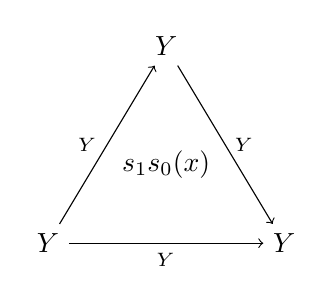
\begin{tikzpicture}
        \node (d1) at (0,0) {$Y$}; \node (d2) at (3,0) {$Y$}; \node (d3) at (1.5,2.5) {$Y$}; 
      \node (c3) at (1.5,1.0) {$s_1s_0(x)$};
      \draw[->] (d1) to node[left] {$\id_Y$} (d3); 
      \draw[->] (d3) to node[right] {$\id_Y$} (d2); 
      \draw[->] (d1) to node[below] {$\id_Y$} (d2); 
      \end{tikzpicture}
    \end{center}
  \end{center}
  4つ組$(s_1s_0(x),\bullet,\si_2,\si_3)$は単体的集合の間の写像$\tau_0: \Lambda^3_1 \to \calC$を定める. 
  \begin{center}
    \begin{tikzpicture}
      \node (a1) at (0,0) {$X$}; \node (a2) at (5,0) {$Y$}; \node (a3) at (3,4.0) {$Y$}; 
      \node (a4) at (5,1.5) {$Y$};
      \draw[->] (a1) to node[above] {$f$} (a3); 
      \draw[->, dashed] (a4) to node[right] {$\id_Y$} (a2); 
      \draw[->, dashed] (a1) to node[below] {$h$} (a2); 
      % \draw[-, line width=5pt, draw=white] (a3) to (a2);
      \draw[->] (a3) to node[left] {$\id_Y$} (a2);
      \draw[->, dashed] (a1) to node[above] {$g$} (a4); 
      \draw[->] (a3) to node[right] {$\id_Y$} (a4); 
    \end{tikzpicture}
  \end{center}
  ただし, 点線はホーン$\Lambda^3_1$における面が「ない」ことをあらわしている. 
  $\calC$は$\infty$-圏であるので, $\tau_0: \Lambda^3_1 \to \calC$を$\tau: \Delta^3 \to \calC$に拡張することができる. 
  面$d_1(\tau)$は$g$から$h$へのホモトピーとみなせる. 
  \begin{center}
    \begin{tikzpicture}
      \node (a0) at (0,0) {$X$}; \node (a1) at (1.5,2.5) {$Y$}; \node (a2) at (3,0) {$Y$}; 
      \draw[->] (a0) to node[left] {$g$} (a1); 
      \draw[->] (a1) to node[right] {$\id_Y$} (a2); 
      \draw[->] (a0) to node[below] {$h$} (a2); 
    \end{tikzpicture}
  \end{center}
\end{Proof}

$f,g: X \to Y$を$\infty$-圏$\calC$における2つの射とする. 
定義1.3.3.1より, $\infty$-圏$\calC$における$f$から$g$へのホモトピーは反転$\infty$-圏$\calC^\OP$における$f$から$g$へのホモトピーとは等しくない. 
しかし, 次の命題が成立する. 

\begin{prop}
  $f,g: X \to Y$を$\infty$-圏$\calC$における2つの射とする. 
  $f$と$g$がホモトピックである必要十分条件は反転$\infty$-圏$\calC^\OP$における射とみなしたときにホモトピックであることである. 
  つまり, 次の2つは同値である. 
  \footnote{
    2つ目の図式において対称律を用いると, これは左ホモトピーと右ホモトピーの同値性を示していることにほかならない. 
  }
  \begin{enumerate}
    \item $d_0(\si)=\id_Y, d_1(\si)=g, d_2(\si)=f$を満たす$2$単体$\si$が存在する. 
    \begin{center}
      \begin{tikzpicture}
        \node (a0) at (0,0) {$X$}; \node (a1) at (1.5,2.5) {$Y$}; \node (a2) at (3,0) {$Y$}; 
        \node (c1) at (1.5,1.0) {$\si$};
        \draw[->] (a0) to node[left] {$f$} (a1); 
        \draw[->] (a1) to node[right] {$\id_Y$} (a2); 
        \draw[->] (a0) to node[below] {$g$} (a2); 
      \end{tikzpicture}
    \end{center}
    \item $d_0(\tau)=f, d_1(\tau)=g, d_2(\tau)=\id_X$を満たす$2$単体$\tau$が存在する. 
    \begin{center}
      \begin{tikzpicture}
        \node (a0) at (0,0) {$X$}; \node (a1) at (1.5,2.5) {$X$}; \node (a2) at (3,0) {$Y$}; 
        \node (c1) at (1.5,1.0) {$\tau$};
        \draw[->] (a0) to node[left] {$\id_X$} (a1); 
        \draw[->] (a1) to node[right] {$f$} (a2); 
        \draw[->] (a0) to node[below] {$g$} (a2); 
      \end{tikzpicture}
    \end{center}
  \end{enumerate}
\end{prop}

\begin{Proof}
  (1)から(2)を示す. 
  $f$と$g$がホモトピックであるとする. 
  対称律より$g$と$f$はホモトピックであるので, これを次のようにあらわす. 
  \begin{center}
    \begin{tikzpicture}
      \node (a0) at (0,0) {$X$}; \node (a1) at (1.5,2.5) {$Y$}; \node (a2) at (3,0) {$Y$};  
      \node (c1) at (1.5,1.0) {$\si$};
      \draw[->] (a0) to node[left] {$g$} (a1); 
      \draw[->] (a1) to node[right] {$\id_Y$} (a2); 
      \draw[->] (a0) to node[below] {$f$} (a2); 
    \end{tikzpicture}
  \end{center}
  $g$と$g$がホモトピックであることをそれぞれ次のようにあらわす. 
  \footnote{
    2つ目の図式は(2)において$f=g$としたものである. 
    図に描いたように$2$単体として$s_0(g)$をとればよい. 
  }
  \begin{center}
    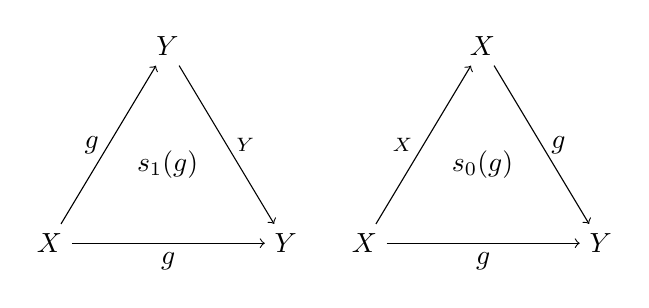
\begin{tikzpicture}
      \node (b0) at (0,0) {$X$}; \node (b1) at (1.5,2.5) {$Y$}; \node (b2) at (3,0) {$Y$}; 
      \node (c2) at (1.5,1.0) {$s_1(g)$};
      \draw[->] (b0) to node[left] {$g$} (b1); 
      \draw[->] (b1) to node[right] {$\id_Y$} (b2); 
      \draw[->] (b0) to node[below] {$g$} (b2); 
      \node (d0) at (4,0) {$X$}; \node (d1) at (5.5,2.5) {$X$}; \node (d2) at (7,0) {$Y$}; 
      \node (c3) at (5.5,1.0) {$s_0(g)$};
      \draw[->] (d0) to node[left] {$\id_X$} (d1); 
      \draw[->] (d1) to node[right] {$g$} (d2); 
      \draw[->] (d0) to node[below] {$g$} (d2); 
    \end{tikzpicture}
  \end{center}
  4つ組$(\si,s_1(g),\bullet,s_0(g))$は単体的集合の間の写像$\rho_0: \Lambda^3_2 \to \calC$を定める. 
  \begin{center}
    \begin{tikzpicture}
      \node (a0) at (0,0) {$X$}; \node (a1) at (3,4.0) {$X$}; \node (a3) at (5,0) {$Y$}; 
      \node (a2) at (5,1.5) {$Y$};
      \draw[->, dashed] (a0) to node[left] {$\id_X$} (a1); 
      \draw[->, dashed] (a1) to node[left] {$f$} (a3); 
      \draw[->, dashed] (a0) to node[below] {$g$} (a3); 
      \draw[->] (a1) to node[right] {$g$} (a2);
      \draw[->] (a0) to node[above] {$g$} (a2); 
      \draw[->] (a2) to node[right] {$\id_Y$} (a3); 
    \end{tikzpicture}
  \end{center}
  ただし, 点線はホーン$\Lambda^3_2$における面が「ない」ことをあらわしている. 
  $\calC$は$\infty$-圏であるので, $\rho_0: \Lambda^3_2 \to \calC$を$\rho: \Delta^3 \to \calC$に拡張することができる. 
  面$d_2(\rho)$は(2)を示している. 
  \begin{center}
    \begin{tikzpicture}
      \node (a0) at (0,0) {$X$}; \node (a1) at (1.5,2.5) {$X$}; \node (a2) at (3,0) {$Y$}; 
      \draw[->] (a0) to node[left] {$\id_X$} (a1); 
      \draw[->] (a1) to node[right] {$f$} (a2); 
      \draw[->] (a0) to node[below] {$g$} (a2); 
    \end{tikzpicture}
  \end{center}
  (2)から(1)も同様に示すことができる. 
\end{Proof}

命題1.3.3.6を用いると, ホモトピーを対称的な形にあらわすことができる. 

\begin{cor}
  $f,g: X \to Y$を$\infty$-圏$\calC$における2つの射とする. 
  $f$と$g$がホモトピックである必要十分条件は, ある単体的集合の間の写像$H: \Delta^1 \ti \Delta^1 \to \calC$が存在して
  \begin{align*}
    H|_{\{0\} \ti \Delta^1}=f, H|_{\{1\} \ti \Delta^1}=g,
    H|_{\Delta^1 \ti \{0\}}=\id_X, H|_{\Delta^1 \ti \{1\}}=\id_Y
  \end{align*}
  を満たすことである. 
  \begin{center}
    \begin{tikzpicture}
      \node (a) at (0,4) {$X$}; \node (b) at (4,4) {$Y$};
      \node (c) at (0,0) {$X$}; \node (d) at (4,0) {$Y$};
      \node (e) at (1,1) {$\tau$};
      \node (f) at (3,3) {$\si$};
      \draw[->] (a) to node[above] {$f$} (b); 
      \draw[->] (a) to node[left] {$\id_X$} (c);
      \draw[->] (b) to node[right] {$\id_Y$} (d);
      \draw[->] (c) to node[below] {$f$} (d); 
      \draw[->] (a) to node[right] {$h$} (d);   
    \end{tikzpicture}
  \end{center}
\end{cor}

\begin{Proof}
  必要条件を示す. 
  $f$と$g$がホモトピックであることを次のようにあらわす. 
  \begin{center}
    \begin{tikzpicture}
      \node (a0) at (0,0) {$X$}; \node (a1) at (1.5,2.5) {$Y$}; \node (a2) at (3,0) {$Y$}; 
      \draw[->] (a0) to node[left] {$f$} (a1); 
      \draw[->] (a1) to node[right] {$\id_Y$} (a2); 
      \draw[->] (a0) to node[below] {$g$} (a2); 
    \end{tikzpicture}
  \end{center}
  このとき, $\tau=s_0(g)$とすればよい. 
  \begin{center}
    \begin{tikzpicture}
      \node (a0) at (0,0) {$X$}; \node (a1) at (1.5,2.5) {$X$}; \node (a2) at (3,0) {$Y$}; 
      \draw[->] (a0) to node[left] {$\id_X$} (a1); 
      \draw[->] (a1) to node[right] {$g$} (a2); 
      \draw[->] (a0) to node[below] {$g$} (a2); 
    \end{tikzpicture}
  \end{center}
  十分条件を示す. 
  次の図式
  \begin{center}
    \begin{tikzpicture}
      \node (a) at (0,4) {$X$}; \node (b) at (4,4) {$Y$};
      \node (c) at (0,0) {$X$}; \node (d) at (4,0) {$Y$};
      \node (e) at (1,1) {$\tau$};
      \node (f) at (3,3) {$\si$};
      \draw[->] (a) to node[above] {$f$} (b); 
      \draw[->] (a) to node[left] {$\id_X$} (c);
      \draw[->] (b) to node[right] {$\id_Y$} (d);
      \draw[->] (c) to node[below] {$f$} (d); 
      \draw[->] (a) to node[right] {$h$} (d);   
    \end{tikzpicture}
  \end{center}
  において, $\si$は$f$と$g$がホモトピック, $\tau$は$g$と$h$がホモトピックであることを示している. 
  対称律と推移律を用いると, $f$と$g$がホモトピックであることがわかる.
\end{Proof}

\subsection{\texorpdfstring{$\infty$}{infty}-圏における射の合成}

$\infty$-圏における射の合成を定義する. 

\begin{definition}
  $f:X \to Y, g: Y \to Z, h: X \to Z$を$\infty$-圏における射とする. 
  $d_0(\si)=g, d_1(\si)=h, d_2(\si)=f$を満たすある$2$単体$\si$が存在するとき, $h$は$f$と$g$の合成(composition)であるという. 
  このとき, $2$単体$\si$は$f$と$g$の合成して$h$を示す($\si$ witnesses $h$ as a composition of $f$ and $g$)という. 
  \begin{center}
    \begin{tikzpicture}
      \node (a0) at (0,0) {$X$}; \node (a1) at (1.5,2.5) {$Y$}; \node (a2) at (3,0) {$Z$}; 
      \node (c1) at (1.5,1.0) {$\si$};
      \draw[->] (a0) to node[left] {$f$} (a1); 
      \draw[->] (a1) to node[right] {$g$} (a2); 
      \draw[->] (a0) to node[below] {$h$} (a2); 
    \end{tikzpicture}
  \end{center}
\end{definition}

定義1.3.4.1では射$h$は$f$と$g$では一意には定まらないが, ホモトピーの違いをのぞいて定まる. 

\begin{prop}
  $f:X \to Y, g: Y \to Z$を$\infty$-圏における射とする. 
  このとき, 次の2つが成立する. 
  \begin{enumerate}
    \item $f$と$g$の合成である射$h: X \to Z$が存在する. 
    \item $h: X \to Z$を$f$と$g$の合成, $h': X \to Z$を同じ域を余域をもつある射とする. 
    このとき, $h': X \to Z$が$f$と$g$の合成である必要十分条件は$h'$と$h$がホモトピックであることである. 
  \end{enumerate}
\end{prop}

\begin{Proof}
  (1)を示す.
  3つ組$(f,\bullet,g)$は単体的集合の間の写像$\si_0: \Lambda^2_1 \to \calC$を定める. 
  \begin{center}
    \begin{tikzpicture}
      \node (a0) at (0,0) {$X$}; \node (a1) at (1.5,2.5) {$Y$}; \node (a2) at (3,0) {$Z$}; 
      \node (c1) at (1.5,1.0) {$\si_0$};
      \draw[->] (a0) to node[left] {$f$} (a1); 
      \draw[->] (a1) to node[right] {$g$} (a2);
    \end{tikzpicture}
  \end{center}
  $\calC$は$\infty$-圏であるので, $\si_0$を$\si: \Delta^2 \to \calC$に拡張することができる.
  \begin{center}
    \begin{tikzpicture}
      \node (a0) at (0,0) {$X$}; \node (a1) at (1.5,2.5) {$Y$}; \node (a2) at (3,0) {$Z$}; 
      \node (c1) at (1.5,1.0) {$\si$};
      \draw[->] (a0) to node[left] {$f$} (a1); 
      \draw[->] (a1) to node[right] {$g$} (a2); 
      \draw[->] (a0) to node[below] {$h$} (a2); 
    \end{tikzpicture}
  \end{center}
  よって, $h:=d_1(\si)$とすれば, $\si$は$f$と$g$の合成として$h=d_1(\si)$を示す. \\
  $h': X \to Z$が$f$と$g$の合成であるとする. 
  $f$と$g$の合成として$h'$を示す$2$単体$\si'$をとってくる. 
  \begin{center}
    \begin{tikzpicture}
      \node (a0) at (0,0) {$X$}; \node (a1) at (1.5,2.5) {$Y$}; \node (a2) at (3,0) {$Z$}; 
      \node (c1) at (1.5,1.0) {$\si'$};
      \draw[->] (a0) to node[left] {$f$} (a1); 
      \draw[->] (a1) to node[right] {$g$} (a2); 
      \draw[->] (a0) to node[below] {$h'$} (a2); 
    \end{tikzpicture}
  \end{center}
  このとき, 4つ組$(s_1(g),\bullet,\si',\si)$は単体的集合の間の写像$\tau_0: \Lambda^3_1 \to \calC$を定める. 
  \begin{center}
    \begin{tikzpicture}
      \node (a0) at (0,0) {$X$}; \node (a1) at (3,4.0) {$Y$}; \node (a3) at (5,0) {$Z$};  
      \node (a2) at (5,1.5) {$Z$};
      \draw[->] (a0) to node[above] {$f$} (a1); 
      \draw[->] (a1) to node[right] {$g$} (a2);
      \draw[->] (a1) to node[left] {$g$} (a3); 
      \draw[->, dashed] (a2) to node[right] {$\id_Z$} (a3); 
      \draw[->, dashed] (a0) to node[below] {$h'$} (a3);
      \draw[->, dashed] (a0) to node[above] {$h$} (a2); 
    \end{tikzpicture}
  \end{center}
  ただし, 点線はホーン$\Lambda^3_1$における面が「ない」ことをあらわしている. 
  $\calC$は$\infty$-圏であるので, $\tau_0: \Lambda^3_1 \to \calC$を$\tau: \Delta^3 \to \calC$に拡張することができる. 
  面$d_1(\tau)$は$h$から$h'$へのホモトピーを示している. 
  \begin{center}
    \begin{tikzpicture}
      \node (a0) at (0,0) {$X$}; \node (a1) at (1.5,2.5) {$Z$}; \node (a2) at (3,0) {$Z$}; 
      \draw[->] (a0) to node[left] {$h$} (a1); 
      \draw[->] (a1) to node[right] {$\id_Z$} (a2); 
      \draw[->] (a0) to node[below] {$h'$} (a2); 
    \end{tikzpicture}
  \end{center}
  (2)の十分条件を示す. 
  $h'$と$h$がホモトピックであるとする. これを次のようにあらわす.
  \begin{center}
    \begin{tikzpicture}
      \node (a0) at (0,0) {$X$}; \node (a1) at (1.5,2.5) {$Z$}; \node (a2) at (3,0) {$Z$}; 
      \node (c1) at (1.5,1.0) {$\si''$};
      \draw[->] (a0) to node[left] {$h$} (a1); 
      \draw[->] (a1) to node[right] {$\id_Z$} (a2); 
      \draw[->] (a0) to node[below] {$h''$} (a2); 
    \end{tikzpicture}
  \end{center}
  4つ組$(s_1(g),\si'',\bullet,\si)$は$\Lambda^3_2 \to \calC$を定める.  
  \begin{center}
    \begin{tikzpicture}
      \node (a0) at (0,0) {$X$}; \node (a1) at (3,4.0) {$Y$}; \node (a3) at (5,0) {$Z$}; 
      \node (a2) at (5,1.5) {$Z$};
      \draw[->, dashed] (a0) to node[above] {$f$} (a1); 
      \draw[->] (a1) to node[right] {$g$} (a2);
      \draw[->, dashed] (a1) to node[left] {$g$} (a3); 
      \draw[->, ] (a2) to node[right] {$\id_Z$} (a3); 
      \draw[->, dashed] (a0) to node[below] {$h'$} (a3);
      \draw[->] (a0) to node[above] {$h$} (a2); 
    \end{tikzpicture}
  \end{center}
  ただし, 点線はホーン$\Lambda^3_2$における面が「ない」ことをあらわしている. 
  $\calC$は$\infty$-圏であるので, $\rho_0: \Lambda^3_2 \to \calC$を$\rho: \Delta^3 \to \calC$に拡張することができる. 
  面$d_2(\rho)$は$h'$が$f$と$g$の合成であることを示している. 
  \begin{center}
    \begin{tikzpicture}
      \node (a0) at (0,0) {$X$}; \node (a1) at (1.5,2.5) {$Y$}; \node (a2) at (3,0) {$Z$}; 
      \draw[->] (a0) to node[left] {$f$} (a1); 
      \draw[->] (a1) to node[right] {$g$} (a2); 
      \draw[->] (a0) to node[below] {$h'$} (a2); 
    \end{tikzpicture}
  \end{center}
\end{Proof}

\begin{nota}
  $f:X \to Y, g: Y \to Z$を$\infty$-圏における射とする. 
  $h$が$f$と$g$の合成であることを$h=g \ci f$とあらわす. 
  これは暗に$f$と$g$の合成として$h$を示す$2$単体が存在するということである. 
  これを単に$f$と$g$の合成としての$h$ ($h$ as the composition of $f$ and $g$)という. 
  これがwell-definedであることは命題1.3.4.7で示す. 
  (命題1.3.4.2では$h$のホモトピー類がwell-definedであることしか示していない.)
\end{nota}

\begin{example}
  $f: X \to Y, g: Y \to Z$を通常の圏$\calC$における射とする. 
  $\infty$-圏$\N(\calC)$における$f$と$g$の合成である射$h: X \to Z$は一意に存在する. 
\end{example}

\begin{Proof}
  例1.3.3.2よりホモトピックである必要十分条件は$h=h'$であったので, 合成は一意に定まる. 
\end{Proof}

\begin{example}
  $X$を位相空間とする. 
  $f(1)=g(0)$を満たす連続写像$f,g: [0,1] \to X$に対して, $f$と$g$をつなげた道$g \star f: [0,1] \to X$を次のように定義する. 
  \begin{align*}
    (g \star f)(t) :=
    \begin{cases}
      f(2t) &(0 \leq t \leq 1/2) \\
      g(2t-1) &(1/2 \leq t \leq 1)
    \end{cases}
  \end{align*}
  このとき, $g \star f$は$\infty$-圏$\Sing_\bullet(X)$における$f$と$g$の合成である. 
  正確にいうと, 連続写像
  \begin{align*}
    \si: |\Delta^2| \to X :
    \si(t_0,t_1,t_2)=
    \begin{cases}
      f(t_1+2t_2) &(t_0 \geq t_2) \\
      g(t_2-t_0) &(t_0 \leq t_2)
    \end{cases}
  \end{align*}
  は$f$と$g$の合成として$g \star f$を示す$2$単体とみなせるということである. 
\end{example}

\begin{Proof}
  構成1.1.7.1を用いて計算すると, $d_0(\si)=g, d_1(\si)=g \star f, d_2(\si)=f$になる. 
  \begin{center}
    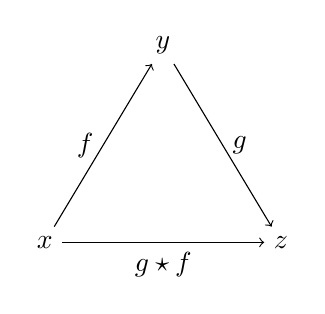
\begin{tikzpicture}
      \node (a0) at (0,0) {$x$}; \node (a1) at (1.5,2.5) {$y$}; \node (a2) at (3,0) {$z$}; 
      \node (c1) at (1.5,1.0) {$\si$};
      \draw[->] (a0) to node[left] {$f$} (a1); 
      \draw[->] (a1) to node[right] {$g$} (a2);
      \draw[->] (a0) to node[below] {$g \star f$} (a2); 
    \end{tikzpicture}
  \end{center}
\end{Proof}

\begin{remark}
  $\infty$-圏$\Sing_\bullet(X)$において, $g \star f$は$f$と$g$の合成として一意には定まらない. 
  命題1.3.4.2より, $X$において$g \star f$とホモトピックな道は同じ性質をもつ. 
  例えば, $g \star f$を次のような道$[0,1] \to X$
  \begin{align*}
    s \mt 
    \begin{cases}
      f(3s) &(0 \leq s \leq 1/3) \\
      g(\frac{3}{2}s-\frac{1}{2}) &(1/3 \leq s \leq 1)
    \end{cases}
  \end{align*}
  に変えてもよい. 
  例1.3.3.3より, $g \star f$は$\infty$-圏$\Sing_\bullet(X)$において, これらの道は$f$と$g$の合成とみなせる. 
\end{remark}

\begin{prop}
  $\infty$-圏$\calC$において, それぞれホモトピックな射$f,f': X \to Y$と$g,g': Y \to Z$が与えられているとする.
  $h$を$f$と$g$の合成, $h'$を$f'$と$g'$の合成とする. 
  このとき, $h$と$h'$はホモトピックである.
\end{prop}

\begin{Proof}
  $h''$を$f$と$g'$の合成とする. 
  $h$と$h'$がそれぞれ$h''$とホモトピックであることを示せば, 推移律より$h$と$h'$はホモトピックであることがわかる. 
  $f$と$g$の合成として$h$を示す$2$単体を$\si_3$, $f$と$g'$の合成として$h''$を示す$2$単体を$\si_2$とする. 
  \begin{center}
    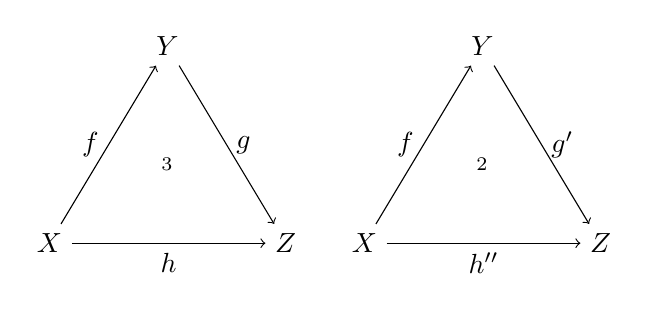
\begin{tikzpicture}
      \node (b0) at (0,0) {$X$}; \node (b1) at (1.5,2.5) {$Y$}; \node (b2) at (3,0) {$Z$}; 
      \node (c2) at (1.5,1.0) {$\si_3$};
      \draw[->] (b0) to node[left] {$f$} (b1); 
      \draw[->] (b1) to node[right] {$g$} (b2); 
      \draw[->] (b0) to node[below] {$h$} (b2); 
      \node (d0) at (4,0) {$X$}; \node (d1) at (5.5,2.5) {$Y$}; \node (d2) at (7,0) {$Z$}; 
      \node (c3) at (5.5,1.0) {$\si_2$};
      \draw[->] (d0) to node[left] {$f$} (d1); 
      \draw[->] (d1) to node[right] {$g'$} (d2); 
      \draw[->] (d0) to node[below] {$h''$} (d2); 
    \end{tikzpicture}
  \end{center}
  $g$から$g'$へのホモトピーを$s_0(g)$とする. 
  \begin{center}
    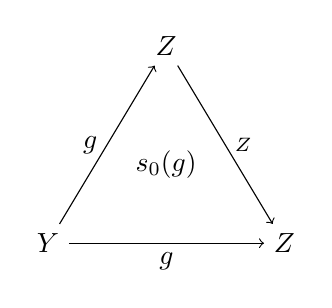
\begin{tikzpicture}
      \node (b0) at (0,0) {$Y$}; \node (b1) at (1.5,2.5) {$Z$}; \node (b2) at (3,0) {$Z$}; 
      \node (c2) at (1.5,1.0) {$s_0(g)$};
      \draw[->] (b0) to node[left] {$g$} (b1); 
      \draw[->] (b1) to node[right] {$\id_Z$} (b2); 
      \draw[->] (b0) to node[below] {$g$} (b2); 
    \end{tikzpicture}
  \end{center}
  4つ組$(s_0(g),\bullet,\si_2,\si_3)$は単体的集合の間の写像$\tau_0: \Lambda^3_1 \to \calC$を定める. 
  \begin{center}
    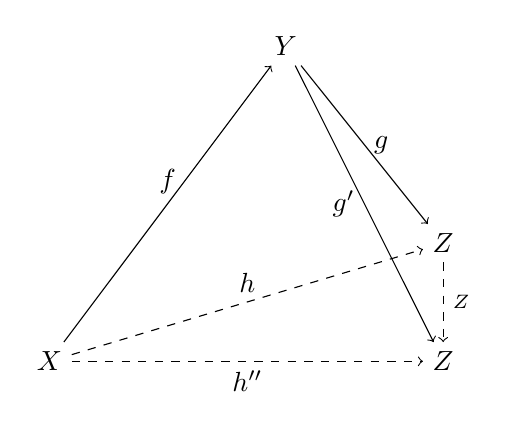
\begin{tikzpicture}
      \node (a0) at (0,0) {$X$}; \node (a1) at (3,4.0) {$Y$}; \node (a3) at (5,0) {$Z$};  
      \node (a2) at (5,1.5) {$Z$};
      \draw[->] (a0) to node[above] {$f$} (a1); 
      \draw[->] (a1) to node[right] {$g$} (a2);
      \draw[->] (a1) to node[left] {$g'$} (a3); 
      \draw[->, dashed] (a0) to node[above] {$h$} (a2); 
      \draw[->, dashed] (a0) to node[below] {$h''$} (a3);
      \draw[->, dashed] (a2) to node[right] {$\id_Z$} (a3); 
    \end{tikzpicture}
  \end{center}
  ただし, 点線はホーン$\Lambda^3_1$における面が「ない」ことをあらわしている. 
  $\calC$は$\infty$-圏であるので, $\tau_0: \Lambda^3_1 \to \calC$を$\tau: \Delta^3 \to \calC$に拡張することができる. 
  面$d_1(\tau)$は$h$から$h''$からのホモトピーを示している. 
  \begin{center}
    \begin{tikzpicture}
      \node (a0) at (0,0) {$X$}; \node (a1) at (1.5,2.5) {$Z$}; \node (a2) at (3,0) {$Z$}; 
      \draw[->] (a0) to node[left] {$h$} (a1); 
      \draw[->] (a1) to node[right] {$\id_Z$} (a2); 
      \draw[->] (a0) to node[below] {$h''$} (a2); 
    \end{tikzpicture}
  \end{center}
  $h'$が$h''$とホモトピックであることも同様に示すことができる. 
\end{Proof}

\subsection{\texorpdfstring{$\infty$}{infty}-圏のホモトピー圏}

任意の位相空間$X$に対して, $X$の基本亜群(fundamental groupoid)と呼ばれる圏$\pi_{\leq 1}(X)$を考えることができる. 
基本亜群の定義に登場する概念(点, 道, ホモトピー, 道の合成)は$X$の特異$n$単体($n \leq 2$)で書き換えることができる. 
よって, 基本亜群$\pi_{\leq 1}(X)$は位相空間$X$の不変量ではなく, 単体的集合$\Sing_\bullet(X)$の不変量と思える. 
この不変量を$\Sing_\bullet(X)$に対してではなく, 一般の$\infty$-圏$\calC$に拡張する. 
このとき, 基本亜群$\pi_{\leq 1}(X)$は$\calC$のホモトピー圏(homotopy category)と呼ばれる圏$\h \calC$に置き換わる. 
一般にホモトピー圏$\h \calC$は亜群ではないことに注意してほしい. 
ホモトピー圏が亜群となる必要十分条件は$\calC$がKan複体である. \cite[\href{https://kerodon.net/tag/019D}{Tag 019D}]{kerodon}

\begin{cons}
  $\calC$を$\infty$-圏とする. 
  対象$X,Y \in \calC$に対して, $X$から$Y$への射のホモトピー類を$\Hom_{\h \calC}(X,Y)$とあらわす. 
  任意の射$f: X \to Y$に対して, $\Hom_{\h \calC}(X,Y)$の元を$[f]$とあらわす. 

  命題1.3.4.2と命題1.3.4.7より, 射$f: X \to Y, g: Y \to Z$と$f$と$g$の合成$h: X \to Z$に対して, 合成則
  \begin{align*}
    \ci: \Hom_{\h \calC}(Y,Z) \ti \Hom_{\h \calC}(X,Y) \to \Hom_{\h \calC}(X,Z): ([g],[f]) \mt [h] 
  \end{align*}
  が一意に存在する. 
  \footnote{
    命題1.3.4.7より, この合成はwell-definedである.
  }
\end{cons}

\begin{prop}
  $\calC$を$\infty$-圏とする. 
  このとき, 
  \begin{enumerate}
    \item 
    合成は結合的である. 
    つまり, 射$f: W \to X, g: X \to Y, h: Y \to Z$に対して, $\Hom_{\h \calC}(Y,Z)$において
    \begin{align*}
      ([h] \ci [g]) \ci [f] = [h] \ci ([g] \ci [f])
    \end{align*}
    が成立する. 
    \item 
    任意の$X \in \calC$に対して, ホモトピー類$[\id_X] \in \Hom_{\h \calC}(X,X)$は結合に関して単位的である. 
    つまり, 射$f: W \to X, g: X \to Y$に対して, 
    \begin{align*}
      [\id_X] \ci [f] = [f] \\
      [g] \ci [\id_X] = [g]
    \end{align*}
    が成立する. 
  \end{enumerate}
\end{prop}

\begin{Proof}
  (1)を示す. 
  $v: X \to Z$を$g$と$h$の合成, $w: W \to Z$を$f$と$v$の合成, $u: W \to Y$を$f$と$g$の合成とする. 
  \begin{center}
    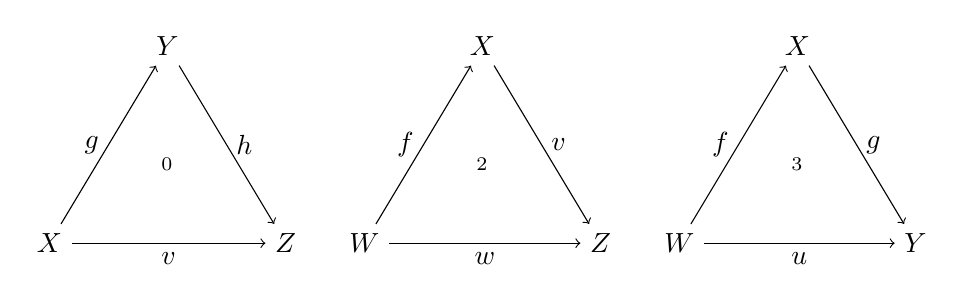
\begin{tikzpicture}
      \node (b0) at (0,0) {$X$}; \node (b1) at (1.5,2.5) {$Y$}; \node (b2) at (3,0) {$Z$}; 
      \node (c2) at (1.5,1.0) {$\si_0$};
      \draw[->] (b0) to node[left] {$g$} (b1); 
      \draw[->] (b1) to node[right] {$h$} (b2); 
      \draw[->] (b0) to node[below] {$v$} (b2); 
      \node (d0) at (4,0) {$W$}; \node (d1) at (5.5,2.5) {$X$}; \node (d2) at (7,0) {$Z$}; 
      \node (c3) at (5.5,1.0) {$\si_2$};
      \draw[->] (d0) to node[left] {$f$} (d1); 
      \draw[->] (d1) to node[right] {$v$} (d2); 
      \draw[->] (d0) to node[below] {$w$} (d2); 
      \node (a0) at (8,0) {$W$}; \node (a1) at (9.5,2.5) {$X$}; \node (a2) at (11,0) {$Y$}; 
      \node (c3) at (9.5,1.0) {$\si_3$};
      \draw[->] (a0) to node[left] {$f$} (a1); 
      \draw[->] (a1) to node[right] {$g$} (a2); 
      \draw[->] (a0) to node[below] {$u$} (a2); 
    \end{tikzpicture}
  \end{center}
  このとき, $([h] \ci [g]) \ci [f] = [w], [h] \ci ([g] \ci [f]) = [h] \ci [u]$である. 
  よって, $w$が$u$と$h$の合成であることを示せばよい. 
  4つ組$(\si_0,\bullet,\si_2,\si_3)$は$\tau_0: \Lambda^3_1 \to \calC$を定める. 
  \begin{center}
    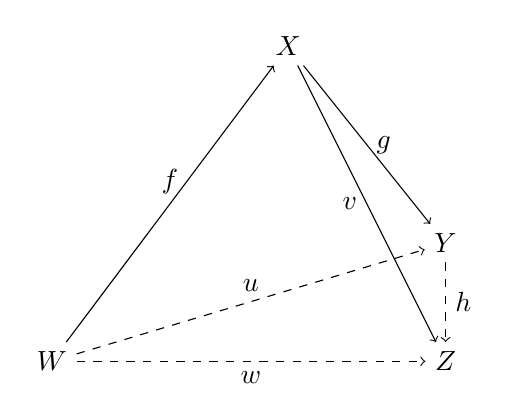
\begin{tikzpicture}
      \node (a0) at (0,0) {$W$}; \node (a1) at (3,4.0) {$X$}; \node (a3) at (5,0) {$Z$};  
      \node (a2) at (5,1.5) {$Y$};
      \draw[->] (a0) to node[above] {$f$} (a1); 
      \draw[->] (a1) to node[right] {$g$} (a2);
      \draw[->] (a1) to node[left] {$v$} (a3); 
      \draw[->, dashed] (a0) to node[above] {$u$} (a2); 
      \draw[->, dashed] (a0) to node[below] {$w$} (a3);
      \draw[->, dashed] (a2) to node[right] {$h$} (a3); 
    \end{tikzpicture}
  \end{center}
  ただし, 点線はホーン$\Lambda^3_1$における面が「ない」ことをあらわしている. 
  $\calC$は$\infty$-圏であるので, $\tau_0: \Lambda^3_1 \to \calC$を$\tau: \Delta^3 \to \calC$に拡張することができる. 
  $d_1(\tau)$は$u$と$h$の合成として$w$を示している. 
  \begin{center}
    \begin{tikzpicture}
      \node (a0) at (0,0) {$W$}; \node (a1) at (1.5,2.5) {$Y$}; \node (a2) at (3,0) {$Z$}; 
      \draw[->] (a0) to node[left] {$u$} (a1); 
      \draw[->] (a1) to node[right] {$h$} (a2); 
      \draw[->] (a0) to node[below] {$w$} (a2); 
    \end{tikzpicture}
  \end{center}
  (2)を示す. 
  $2$単体は$s_0(g)$は$\id_X$と$g$の合成として$g$を示している. 
  $2$単体は$s_1(f)$は$\id_X$と$f$の合成として$f$を示している. 
  \begin{center}
    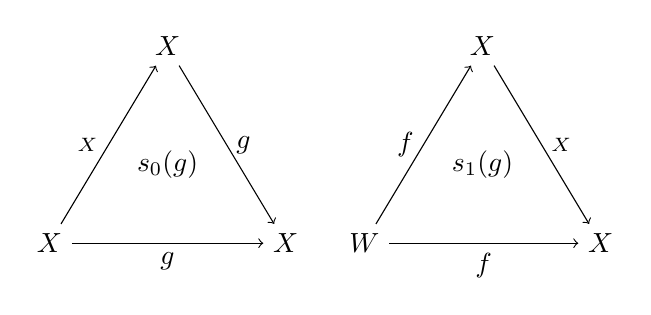
\begin{tikzpicture}
      \node (b0) at (0,0) {$X$}; \node (b1) at (1.5,2.5) {$X$}; \node (b2) at (3,0) {$X$}; 
      \node (c2) at (1.5,1.0) {$s_0(g)$};
      \draw[->] (b0) to node[left] {$\id_X$} (b1); 
      \draw[->] (b1) to node[right] {$g$} (b2); 
      \draw[->] (b0) to node[below] {$g$} (b2); 
      \node (d0) at (4,0) {$W$}; \node (d1) at (5.5,2.5) {$X$}; \node (d2) at (7,0) {$X$}; 
      \node (c3) at (5.5,1.0) {$s_1(g)$};
      \draw[->] (d0) to node[left] {$f$} (d1); 
      \draw[->] (d1) to node[right] {$\id_X$} (d2); 
      \draw[->] (d0) to node[below] {$f$} (d2); 
    \end{tikzpicture}
  \end{center}
\end{Proof}

構成1.3.5.1と命題1.3.5.2より, 圏を定義することができる. 

\begin{definition}
  $\calC$を$\infty$-圏とする. 
  圏$\h \calC$を次のように定義することができる. 
  \begin{itemize}
    \item $\h \calC$の対象は$\calC$の対象
    \item $X,Y \in \calC$に対して, $\infty$-圏$\calC$における$X$から$Y$への射のホモトピー類の集まりを$\Hom_{\h \calC}(X,Y)$とする. 
    \item 任意の対象$X \in \calC$に対して, $\h \calC$における恒等射はホモトピー類$[\id_X]$
    \item 射の合成は構成1.3.5.1で与えた対応
  \end{itemize}
  圏$\h \calC$を$\infty$-圏$\calC$のホモトピー圏(homotopy category)という.
  \footnote{
    2章5節のホモトピー圏は一般の単体的集合に対して随伴の形で定義されたが, ここでは$\infty$-圏に対してのみ定義された概念であることに注意. 
    しかし, $\infty$-圏においてこの2つのホモトピー圏は圏同型となる. (命題1.3.5.7)
  } 
\end{definition}

\begin{example}
  $\calC$を通常の圏とする. 
  例1.3.1.3と例1.3.3.2より, $\infty$-圏$\N(\calC)$のホモトピー圏$\h \N(\calC)$は通常の圏と同一視できる. 
  特に, ホモトピー圏$\h \Delta^n$は$[n]$と同一視できる. 
\end{example}

\begin{example}
  $X$を位相空間, $\Sing_\bullet(X)$を$\infty$-圏とみなす. 
  例1.3.1.4と例1.3.3.3と練習1.3.3.4より, ホモトピー圏$\h \Sing_\bullet(X)$は基本亜群$\pi_{\leq 1}(X)$と同一視できる. 
\end{example}

$\calC$を$\infty$-圏とする. 
注意1.2.5.3と定義1.3.5.3で2つのホモトピー圏を定義したことを確認する. 
\begin{itemize}
  \item 
  注意1.2.5.3のホモトピー圏は任意の単体的集合$\S$に対して, $\Hom$の間の関係式で定義された. 
  \item 
  定義1.3.5.3のホモトピー圏は$\calC$が$\infty$-圏である場合に定義された. 
\end{itemize}

\begin{cons}
  $\infty$-圏$\calC$の$n$単体を$\si: \Delta^n \to \calC$とあらわす. 
  $0 \leq i \leq n$に対して, $\Delta^n$の$i$番目の点の像を$C_i$とあらわす. 
  $0 \leq i \leq j \leq n$に対して, $i$番目の点と$j$番目の点をつなげる$\Delta^n$の辺の像を$f_{ij}$とあらわす. 
  射$f_{ij}$のホモトピー類を$[f_{ij}] \in \Hom_{\h \calC}(C_i,C_j)$とあらわす. 
  このとき, $(\{C_i\}_{0 \leq i \leq n}, \{[f_{ij}]\}_{0 \leq i \leq j \leq n})$は圏$\simop$からホモトピー圏$\h \calC$への関手とみなせる. 
  $\h \calC$のnerve $\N(\h \calC)$の$n$単体を$u(\si)$とあらわす. 
  このとき, 構成$\si \mt u(\si)$は単体的集合の間の写像
  \begin{align*}
    u: \calC \to \N(\h \calC)
  \end{align*}
  を定める. 
\end{cons}

構成1.3.5.6の写像は次のような普遍性をもつ. 

\begin{prop}
  $\calC$を$\infty$-圏, $u: \calC \to \N(\h \calC)$を構成1.3.5.6の写像とする. 
  このとき, 定義1.2.5.1の意味で$u$は($\infty$-圏を単に単体的集合とみなした) $\calC$のホモトピー圏として$\h \calC$を示す. 
  つまり, 任意の圏$\calD$に対して, 合成
  \begin{align*}
    \Hom_{\cat}(\h \calC,\calD) \to \Hom_{\sset}(\N(\h \calC), \N(D)) \xr{- \ci u} \Hom_{\sset}(\calC,\N(D))
  \end{align*}
  は全単射である. 
  \footnote{
    つまり, 定義1.3.5.3のホモトピー圏が定義1.2.5.1のホモトピー圏の定義を満たしていることを示している. 
  }
\end{prop}

\begin{Proof}
  $G: \h\calC \to \calD$をホモトピー圏の間の関手とする, 
  このとき, 単体的集合の間の写像$F: \calC \to \N(\calD)$を合成
  \begin{align*}
    \calC \xr{u} \N(\h\calC) \xr{\N(G)} \N(\calD) 
  \end{align*}
  として定義する. 

\end{Proof}

\subsection{\texorpdfstring{$\infty$}{infty}-圏における同型射}

通常の圏における同型射の概念を$\infty$-圏においても考える. 

\begin{definition}
  $f: X \to Y$を$\infty$-圏$\calC$における射とする. 
  ホモトピー圏$\h \calC$においてホモトピー類$[f]$が(通常の意味で)同型射であるとき, $f$を同型射(isomorphism)という.
  同型射$f: X \to Y$が存在するとき, 2つの対象$X,Y \in \calC$は同型(isomorphic)であるという. 
  つまり, ホモトピー圏$\h \calC$において$X$と$Y$が(通常の意味で)同型である.
\end{definition}

\begin{example}
  $\calC$を通常の圏とする. 
  例1.3.5.4より$\h \N(\calC) \simeq \calC$なので, $\infty$-圏$\N (\calC)$において射$f: X \to Y$が同型射である必要十分条件は$\calC$において同型射であることである. 
\end{example}

\begin{remark}[two-out-of-three]
  $f: X \to Y, g: Y \to Z$を$\infty$-圏$\calC$における射, $h$を$f$と$g$の合成とする. 
  $f,g,h$のうち2つが同型射であれば, 残り1つも同型射である. 
\end{remark}

\begin{definition}
  $f: X \to Y, g: Y \to X$を$\infty$-圏$\calC$における射とする. 
  $f$と$g$の合成が$\id_X$であるとき, $g$は$f$の左ホモトピー逆射(left homotopy inverse)という. 
  つまり, ホモトピー圏$\h \calC$において, $[\id_X]=[g] \ci [f]$が成立する. 
  \begin{center}
    \begin{tikzpicture}
      \node (a0) at (0,0) {$X$}; \node (a1) at (1.5,2.5) {$Y$}; \node (a2) at (3,0) {$X$}; 
      \draw[->] (a0) to node[left] {$f$} (a1); 
      \draw[->] (a1) to node[right] {$g$} (a2); 
      \draw[->] (a0) to node[below] {$\id_X$} (a2); 
    \end{tikzpicture}
  \end{center}
  $g$と$f$の合成が$\id_Y$であるとき, $g$は$f$の右ホモトピー逆射(right homotopy inverse)という. 
  つまり, ホモトピー圏$\h \calC$において, $[\id_Y]=[f] \ci [g]$が成立する. 
  \begin{center}
    \begin{tikzpicture}
      \node (a0) at (0,0) {$Y$}; \node (a1) at (1.5,2.5) {$X$}; \node (a2) at (3,0) {$Y$}; 
      \draw[->] (a0) to node[left] {$g$} (a1); 
      \draw[->] (a1) to node[right] {$f$} (a2); 
      \draw[->] (a0) to node[below] {$\id_Y$} (a2); 
    \end{tikzpicture}
  \end{center}
  $g$が$f$の左ホモトピー逆射かつ右ホモトピー逆射であるとき, $g$は$f$のホモトピー逆射(homotopy inverse)という. 
\end{definition}

\begin{remark}
  $f: X \to Y, g: Y \to X$を$\infty$-圏$\calC$における射とする. 
  $\infty$-圏における同型の定義がホモトピー類を用いて定義されているので, $g$が$f$の左ホモトピー逆射(右ホモトピー逆射, ホモトピー逆射)であるかは$[f]$と$[g]$のホモトピーにのみによる. 
\end{remark}

\begin{remark}
  $f: X \to Y, g: Y \to X$を$\infty$-圏$\calC$における射とする. 
  $g$が$f$の左ホモトピー逆射である必要十分条件は$f$が$g$の右ホモトピー逆射であることである. 
  この2つの条件は$d_0(\si)=g, d_1(\si)=\id_X, d_2(\si)=f$を満たす$2$単体$\si$が存在することと同値である. 
  \begin{center}
    \begin{tikzpicture}
      \node (a0) at (0,0) {$X$}; \node (a1) at (1.5,2.5) {$Y$}; \node (a2) at (3,0) {$X$};
      \node (c2) at (1.5,1.0) {$\si$}; 
      \draw[->] (a0) to node[left] {$f$} (a1); 
      \draw[->] (a1) to node[right] {$g$} (a2); 
      \draw[->] (a0) to node[below] {$\id_X$} (a2); 
    \end{tikzpicture}
  \end{center}
\end{remark}

\begin{remark}
  $f: X \to Y$を$\infty$-圏$\calC$における射とする. 
  $f$が左ホモトピー逆射$g$と右ホモトピー逆射$h$をもつとする. 
  \begin{center}
    \begin{tikzpicture}
      \node (a0) at (0,0) {$X$}; \node (a1) at (1.5,2.5) {$Y$}; \node (a2) at (3,0) {$X$}; 
      \draw[->] (a0) to node[left] {$f$} (a1); 
      \draw[->] (a1) to node[right] {$g$} (a2); 
      \draw[->] (a0) to node[below] {$\id_X$} (a2); 
      \node (b0) at (4,0) {$Y$}; \node (b1) at (5.5,2.5) {$X$}; \node (b2) at (7,0) {$Y$}; 
      \draw[->] (b0) to node[left] {$h$} (b1); 
      \draw[->] (b1) to node[right] {$f$} (b2); 
      \draw[->] (b0) to node[below] {$\id_Y$} (b2); 
    \end{tikzpicture}
  \end{center}
  このとき, $g$と$h$はホモトピックである. 
  よって, $g$も$h$も$f$のホモトピー逆射である. 
\end{remark}

\begin{Proof}
  ホモトピー圏において
  \begin{align*}
    [g]=[g] \ci [\id_Y] = [g] \ci ([h] \ci [f]) = ([g] \ci [h]) \ci [f]
    =[\id_X] \ci [h] =[h]
  \end{align*}
  が成立することから分かる. 
\end{Proof}

\begin{remark}
  $f: X \to Y$を$\infty$-圏$\calC$における射とする. 
  注意1.3.6.7より, 次の3つは同値である. 
  \begin{enumerate}
    \item 射$f$は同型射である. 
    \item 射$f$はホモトピー逆射$g$をもつ. 
    \item $f$は左ホモトピー逆射と右ホモトピー逆射をもつ. 
  \end{enumerate}
\end{remark}

このとき, 射$g$はホモトピー同値の違いをのぞいて一意に定まる. 
さらに, 任意の$f$の左, 右ホモトピー逆射は$g$とホモトピックである. 
よって, $f$のホモトピー逆射を$f^{-1}$と書くことがある. 

\begin{remark}
  $f: X \to Y$を$\infty$-圏$\calC$における射, $g,h: Y \to X$を$f$の左ホモトピー逆射とする. 
  $f$が右ホモトピー逆射をもたないとき, $g$と$h$がホモトピックであるとは限らない. 
\end{remark}

\begin{prop}
  $\calC$をKan複体とする. 
  このとき, $\calC$における任意の射は同型射である. 
\end{prop}

\begin{Proof}
  $f: X \to Y$を$\infty$-圏$\calC$における射とする. 
  3つ組$(\bullet,\id_X,f)$は単体的集合の間の写像$\si_0: \Lambda^2_0 \to \calC$を定める. 
  \begin{center}
    \begin{tikzpicture}
      \node (a0) at (0,0) {$X$}; \node (a1) at (1.5,2.5) {$Y$}; \node (a2) at (3,0) {$X$}; 
      \node (c1) at (1.5,1.0) {$\si_0$};
      \draw[->] (a0) to node[left] {$f$} (a1); 
      \draw[->, dashed] (a1) to (a2); 
      \draw[->] (a0) to node[below] {$\id_X$} (a2); 
    \end{tikzpicture}
  \end{center}
  $\calC$はKan複体なので, $\si_0$を$\si: \Delta^2 \to \calC$に拡張することができる. 
  \begin{center}
    \begin{tikzpicture}
      \node (a0) at (0,0) {$X$}; \node (a1) at (1.5,2.5) {$Y$}; \node (a2) at (3,0) {$X$}; 
      \node (c1) at (1.5,1.0) {$\si$}; 
      \draw[->] (a0) to node[left] {$f$} (a1); 
      \draw[->] (a1) to node[right] {$d_0(\si)$} (a2); 
      \draw[->] (a0) to node[below] {$\id_X$} (a2); 
    \end{tikzpicture}
  \end{center}
  $g:=d_0(\si)$とおくと, $g$は$f$の左ホモトピー逆射である. 
  $\tau_0: \Lambda^2_2 \to \calC$を考えると$f$が右ホモトピー逆射をもつことも分かる. 
  注意1.3.6.8より, $f$は同型射である. 
\end{Proof}

\begin{remark}
  命題1.3.6.10の逆も成立する. 
  つまり, $\infty$-圏$\calC$における任意の射が可逆であれば, $\calC$はKan複体である. 
  証明は\cite[\href{https://kerodon.net/tag/019D}{Tag 019D}]{kerodon}を参照. 
\end{remark}

\begin{definition}
  $\S$をKan複体とする. 
  命題1.3.6.10より, 定義1.3.5.3のホモトピー圏$\h \S$は亜群である. 
  この亜群を$\pi_{\leq 1}(\S)$とあらわし, $\S$の基本亜群(fundamental groupoid)という. 
\end{definition}

\begin{remark}
  $\S$をKan複体とする. 
  ホモトピー圏の定義より, $\pi_{\leq 1}(\S)$の対象は$\S$の点である.
  Kan複体は任意の射が可逆であるので, 点$x,y \in S_0$が$\pi_{\leq 1}(\S)$において同型である必要十分条件は, $\S$において辺$e: x \to y$が存在することである. 
  命題1.1.9.10より, 点$x,y \in S_0$が$\pi_{\leq 1}(\S)$において同型である必要十分条件は, $x$と$y$が$\S$の同じ連結成分に属することである. 
  つまり, 自然な全単射
  \begin{align*}
    \pi_0(\S) \simeq \{\pi_{\leq 1}(\S)\text{の対象}\} / \text{同型射}
  \end{align*}
  が存在する. 
\end{remark}

\begin{example}
  $X$を位相空間とする. 
  特異単体的集合$\Sing_\bullet(X)$はKan複体であるので, 基本亜群$\pi_{\leq 1}(\Sing_\bullet(X))$は位相空間$X$の基本亜群$\pi_{\leq 1}(X)$とみなせる.
\end{example}

\newpage

\section{\texorpdfstring{$\infty$}{infty}-圏の関手}

$\calC,\calD$を通常の圏, $\N(\calC), \N(\calD)$を$\infty$-圏とする. 
命題1.2.2.1より, nerve関手$\N$は全単射
\begin{align*}
  \{\text{関手}F: \calC \to \calD\} 
  \simeq \{\text{単体的集合の間の写像} ~\N(\calC) \to \N(\calD)\}
\end{align*}
を誘導する. 
この考えを一般化して, 通常の圏の関手を$\infty$-圏においても考える. 

\begin{definition}
  $\calC,\calD$を$\infty$-圏とする.
  $\calC$から$\calD$への関手とは単体的集合の間の写像$F: \calC \to \calD$である.  
\end{definition}

4章では$\infty$-圏の間の関手を学ぶことが目標である. 
4章1節ではnerve $\N(\calC)$と特異単体的集合$\Sing_\bullet(X)$における例を説明する. 

通常の圏論では, 関手$F: \calC \to \calD$は$\calC$の対象で添字された点と$\calC$の射で添字された辺による$\calD$における可換図式(commutative diagram)と思える. 
この考えは非常に有用である. 
圏$\calC$が局所小圏であれば, 関手のデータを図式に対応するグラフであらわすことができる. 
4章2節では$\infty$-圏における可換図式を定義して, 高次圏論における図式的な説明から生じる危険について論じる. 

$\calC,\calD$が通常の圏であれば, $\calC$から$\calD$への関手全体は$\fun(\calC,\calD)$とあらわされる圏をなす. 
4章3節では$\infty$-圏におけるこの構成を考える. 
単体的集合$\S,\T$に対して, 点が$\S$から$\T$への写像全体である新しい単体的集合$\fun(\S,\T)$を構成する. 
4章の主目的は$\T$が$\infty$-圏であれば, $\fun(\S,\T)$も$\infty$-圏であることを示すことである. (定理1.4.3.7)
更に, $\S,\T$がある圏$\calC,\calD$のnerveに同型であれば, $\infty$-圏$\fun(\S,\T)$も圏$\fun(\calC,\calD)$のnerveに圏同値である. 

定理1.4.3.7を示すためにアイデアをいくつか述べる. 
$\infty$-圏$\calC$において, $f: X \to Y$と$g: Y \to Z$が合成可能な射であるとき, $d_0(\si)=g, d_2(\si)=f$を満たす$2$単体$\si$をとってきて, $f$と$g$を合成することができる. 
\begin{center}
  \begin{tikzpicture}
    \node (a0) at (0,0) {$X$}; \node (a1) at (1.5,2.5) {$Y$}; \node (a2) at (3,0) {$Z$}; 
    \node (c1) at (1.5,1.0) {$\si$};
    \draw[->] (a0) to node[left] {$f$} (a1); 
    \draw[->] (a1) to node[right] {$g$} (a2); 
    \draw[->] (a0) to node[below] {$g \ci f$} (a2); 
  \end{tikzpicture}
\end{center}

命題1.3.4.2で合成射$g \ci f$がホモトピーの違いをのぞいてwell-definedであることを示した. 
4章6節では$2$単体$\si$がunique up to a contractible space of choicesであることを証明する.
4章7節ではより一般のパスカテゴリーに拡張する.
更に, この一意性のより強い主張が$\calC$が$\infty$-圏と同値であるとき, $\infty$-圏$\fun(\calC,\calD)$が存在することと同値であることを見る.  (命題1.4.6.1)
定理1.4.6.1を証明するためには圏論的なリフトの性質と単体的集合のホモトピー論が必要なので, 4章4節と4章5節でそれぞれ紹介する. 

\subsection{\texorpdfstring{$\infty$}{infty}-圏の関手の例}

定義1.4.0.1の例をいくつか見る. 

\begin{example}
  $\calC,\calD$を通常の圏とする. 
  命題1.2.2.1よりnerveは忠実充満なので, 全単射
  \begin{center}
    \begin{tikzpicture}
      \node (a) at (0,2) {\{通常の圏の間の関手$F: \calC \to \calD$\}};
      \node (b) at (0,0) {\{$\infty$-圏の間の関手$\N(\calC) \to \N(\calD)$\}};
      \draw[->] (a) to node[right] {$\simeq$} (b);
    \end{tikzpicture}
  \end{center}
  を誘導する.
  つまり, 定義1.4.0.1は通常の関手の概念を$\infty$-圏において一般化したものと思うことができる. 
\end{example}

\begin{example}
  $\calC$を$\infty$-圏, $\calD$を通常の圏とする. 
  命題1.3.5.7よりホモトピー圏をとる操作とnerveをとる操作は随伴なので, 全単射
  \begin{center}
    \begin{tikzpicture}
      \node (a) at (0,2) {\{$\infty$-圏の間の関手$\calC \to \N(\calD)$\}};
      \node (b) at (0,0) {\{通常の圏の間の写像$\h \calC \to \calD$\}};
      \draw[->] (a) to node[right] {$\simeq$} (b);
    \end{tikzpicture}
  \end{center}
  を誘導する. 
\end{example}

\begin{remark}
  $F: \calC \to \calD$を$\infty$-圏の間の関手とする. 
  このとき, 
  \begin{enumerate}
    \item 
    各対象$X \in \calC$に対して, 関手$F$は$\calD$の対象を与える. 
    この対象を$F(X)$や単に$FX$とあらわす. 
    \item 
    $\calC$における各射$f: X \to Y$に対して, 関手$F$は$\calD$の射を与える. 
    この射を$F(f): F(X) \to F(Y)$や単に$Ff: FX \to FY$とあらわす. 
    \item 
    任意の対象$X \in \calC$に対して, 関手$F$は恒等射(退化な辺) $\id_X: X \to X$を$\calD$における恒等射$\id_{FX}: FX \to FX$にうつす. 
    \item 
    $\calC$のおける射$f: X \to Y, g: Y \to Z$と$f$と$g$の合成$h$に対して, 射$Fh: FX \to FZ$は$Ff$と$Fg$の合成である. 
  \end{enumerate}
\end{remark}

\begin{remark}
  通常の圏$\calC$から通常の圏$\calD$への関手$F$を定義するためには, 注意1.4.1.3の(1)と(2)にあるように$F$の値を定めて, (3)と(4)にあるように合成と恒等射が関手を交換することを確かめればよい. 
  $\infty$-圏においてはこれだけでは不十分である. 
  $\infty$-圏の間の関手$F: \calC \to \calD$を与えるためには, 「すべての」次元の単体の値を定めなければならない. 
  大雑把にいうと, $F$がコヒーレントホモトピーの違いをのぞいて(up to coherent homotopy)結合と交換するであることを必要とするということである. 
  例えば, 射$f: X \to Y, g: Y \to Z, h:X \to Z$に対して, (4)は$h$が$f$と$g$の合成であるとき, $Fh$は$Ff$と$Fg$の合成であることをあらわしている.
  つまり, これは$2$単体$\si$が$f$と$g$の合成として$h$を示しているとき, $F\si$は$Ff$と$Fg$の合成として$Fh$を示している. 
\end{remark}

\begin{remark}
  $F: \calC \to \calD$を$\infty$-圏の間の関手とする. 
  $\calC$において$f,g: X \to Y$がホモトピックであれば, $\calD$において$Ff,Fg: FX \to FY$はホモトピックである.
  つまり, 関手$F$は$f$から$g$へのホモトピー($2$単体)を$Ff$から$Fg$へのホモトピー($2$単体)にうつす. 
  \begin{center}
    \begin{tikzpicture}
      \node (a0) at (0,0) {$X$}; \node (a1) at (1.5,2.5) {$Y$}; \node (a2) at (3,0) {$Y$}; 
      \draw[->] (a0) to node[left] {$f$} (a1); 
      \draw[->] (a1) to node[right] {$\id_Y$} (a2); 
      \draw[->] (a0) to node[below] {$g$} (a2); 
      \draw[->] (3,2) to[bend left=30] node[above] {$F$} (6,2); 
      \node (b0) at (6,0) {$FX$}; \node (b1) at (7.5,2.5) {$FY$}; \node (b2) at (9,0) {$FY$}; 
      \draw[->] (b0) to node[left] {$Ff$} (b1); 
      \draw[->] (b1) to node[right] {$\id_{FY}$} (b2); 
      \draw[->] (b0) to node[below] {$Fg$} (b2); 
    \end{tikzpicture}
  \end{center}
\end{remark}

\begin{remark}
  $F: \calC \to \calD$を$\infty$-圏の間の関手とする. 
  $f: X \to Y$に対して, $g: Y \to X$が$f$のホモトピー逆射であるとき, $Fg$は$Ff$のホモトピー逆射である. 
  \begin{center}
    \begin{tikzpicture}
      \node (a0) at (0,0) {$X$}; \node (a1) at (1.5,2.5) {$Y$}; \node (a2) at (3,0) {$X$}; 
      \draw[->] (a0) to node[left] {$f$} (a1); 
      \draw[->] (a1) to node[right] {$g$} (a2); 
      \draw[->] (a0) to node[below] {$\id_X$} (a2); 
      \draw[->] (3,2) to[bend left=30] node[above] {$F$} (6,2); 
      \node (b0) at (6,0) {$FX$}; \node (b1) at (7.5,2.5) {$FY$}; \node (b2) at (9,0) {$FX$}; 
      \draw[->] (b0) to node[left] {$Ff$} (b1); 
      \draw[->] (b1) to node[right] {$Fg$} (b2); 
      \draw[->] (b0) to node[below] {$\id_{FX}$} (b2); 
    \end{tikzpicture}
  \end{center}
  特に, 注意1.3.6.8より, $f$が同型射なら$Ff$も同型射である.  
\end{remark}

\begin{example}
  $X$を位相空間, $\calC$を通常の圏とする. 
  $\infty$-圏の間の関手$F: \Sing_\bullet(X) \to \N(\calC)$を定める. 
  $\Sing_\bullet(X)$の$n$単体$\si: |\Delta^n| \to X$に対して, $F(\si)$を次の図式
  \begin{center}
    \begin{tikzpicture}
      \node (c0) at (0,0) {$C_0$}; \node (c1) at (2,0) {$C_1$}; 
      \node (c2) at (4,0) {$\cdots$}; \node (cn) at (6,0) {$C_n$};
      \draw[->] (c0) to node[above] {$f_1$} (c1);
      \draw[->] (c1) to (c2);
      \draw[->] (c2) to node[above] {$f_n$} (cn);
    \end{tikzpicture}
  \end{center}
  として定義する. 
  特に, 例1.3.1.3と例1.3.1.4(例1.1.7.2)より
  \begin{enumerate}
    \item 
    各点$x \in X$に対して, 関手$F$は$\calC$の対象$Fx$を与える. 
    \item 
    $x=f(0), y=f(1)$を満たす各連続な道$f: [0,1] \to X$に対して, 関手$F$は$\calC$の射$Ff: Fx \to Fy$を与える. 
    $\Sing_\bullet(X)$はKan複体なので, 命題1.3.6.10と命題1.4.1.6より$Ff$は同型射である. 
    \item 
    各連続写像$\si: |\Delta^2| \to X$の境界は次のように描ける. 
    \begin{center}
      \begin{tikzpicture}
        \node (a0) at (0,0) {$x$}; \node (a1) at (1.5,2.5) {$y$}; \node (a2) at (3,0) {$z$}; 
        \draw[->] (a0) to node[left] {$f$} (a1); 
        \draw[->] (a1) to node[right] {$g$} (a2); 
        \draw[->] (a0) to node[below] {$h$} (a2); 
      \end{tikzpicture}
    \end{center}
    よって, $\Hom_{\calC}(Fx,Fz)$において, $Fh=Fg \ci Ff$が成立する. 
  \end{enumerate}
  条件(3)を満たす対象の集まり$\{Fx\}_{x \in X}$と同型射の集まり$\{Ff\}_{f: [0,1] \to X}$は$X$上の$\calC$に値をもつ局所系($\calC$-valued local system on $X$)と呼ばれる. 
  今までの議論から, 次の全単射
  \begin{center}
    \begin{tikzpicture}
      \node (a) at (0,2) {\{$\infty$-圏の間の関手$\Sing_\bullet(X) \to \N(\calC)$\}};
      \node (b) at (0,0) {\{$X$上の$\calC$に値をもつ局所系\}};
      \draw[->] (a) to node[right] {$\simeq$} (b);
    \end{tikzpicture}
  \end{center}
  が存在する. 
  例1.3.6.14と例1.4.1.2の全単射から, 次の全単射 
  \begin{center}
    \begin{tikzpicture}
      \node (a) at (0,2) {\{通常の圏の間の関手$\pi_{\leq 1}(X) \to \calC$\}};
      \node (b) at (0,0) {\{$X$上の$\calC$に値をもつ局所系\}};
      \draw[->] (a) to node[right] {$\simeq$} (b);
    \end{tikzpicture}
  \end{center}
  も存在する.
\end{example}

\begin{remark}
  $X$を位相空間, $\calC$を$\infty$-圏とする. 
  例1.4.1.7を一般化して, $X$上の$\calC$に値をもつ局所系を$\infty$-圏の間の関手$\Sing_\bullet(X) \to \calC$として定義する. 
  \begin{center}
    \begin{tikzpicture}
      \node (a) at (0,2) {\{$\infty$-圏の間の関手$\Sing_\bullet(X) \to \calC$\}};
      \node (b) at (0,0) {\{$X$上の$\calC$に値をもつ局所系\}};
      \draw[->] (a) to node[right] {$\simeq$} (b);
    \end{tikzpicture}
  \end{center}
  $\calC$はある圏のnerveであるとは限らないので, $\pi_{\leq 1}(X)$を用いてあらわすことはできない. 
\end{remark}

\begin{example}
  $X$を位相空間, $\calC$を$\infty$-圏とする. 
  系1.1.8.5より特異単体的集合をとる操作と幾何学的実現をとる操作は随伴なので, 全単射
  \begin{center}
    \begin{tikzpicture}
      \node (a) at (0,2) {\{$\infty$-圏の間の関手$\calC \to \Sing_\bullet(X)$\}};
      \node (b) at (0,0) {\{連続写像$|\calC| \to X$\}};
      \draw[->] (a) to node[right] {$\simeq$} (b);
    \end{tikzpicture}
  \end{center}
  が存在する. 
  $\calC$がnerveであっても, どちらの集合も通常の圏の間の関手に置き換えることはできない.
\end{example}

\subsection{\texorpdfstring{$\infty$}{infty}-圏論における可換図式}

\subsection{関手\texorpdfstring{$\infty$}{infty}-圏}

$\calC,\calD$を通常の圏とする.
このとき, $\calC$から$\calD$への関手を対象, 関手の間の自然変換を射とする圏$\fun(\calC,\calD)$が考えられる. 
この構成を$\infty$-圏においても考えてみる. 

\begin{cons}
  $\S,\T$を単体的集合とする. 
  このとき, 構成 
  \begin{align*}
    [n] \mt \Hom_{\sset}(\Delta^n \ti \S,\T)
  \end{align*}
  は$\simop$から$\cset$への関手を定める. 
  この関手を単体的集合とみなし, $\fun(\S,\T)$とあらわす. 
  \footnote{
    $\fun(\S,\T)$の$n$単体$\fun(\S,\T)_n$は$\Hom_{\sset}(\Delta^n \ti \S,\T)$で与えられる. 
    $\al: [m] \to [n]$に対して, $\Hom_{\sset}(\Delta^n \ti \S,\T) \to \Hom_{\sset}(\Delta^m \ti \S,\T)$は
    \begin{align*}
      (\Delta^n \ti \S \to Y) \mt (\Delta^m \ti \S \xr{\al^* \ti \id} \Delta^n \ti \S \to \T)
    \end{align*}
    で与える. 
    ここで, $\al^*$は$\al: [m] \to [n]$から誘導される写像$\Delta^m \to \Delta^n$である. 
  }
\end{cons}

$\fun(\S,\T)$の$n$単体$f$と$\S$の$n$単体$\si$に対して, $\T$の$n$単体$\eva(f,\si)$を合成
\begin{align*}
  \Delta^n \xr{\delta} \Delta^n \ti \Delta^n \xr{\id \ti \si} \Delta^n \ti \S \to \T
\end{align*}
で与える. 
この構成は単体的集合の間の写像
\begin{align*}
  \eva: \fun(\S,\T) \ti \S \to \T : (f,\si) \mt \eva(f,\si):=f(\id,\si)
\end{align*}
を定める. 
この写像を評価写像(evaluation map)という.

\begin{prop}
  $\S,\T,\U$を単体的集合とする. 
  このとき, 合成
  \begin{align*}
    \theta: \Hom_{\sset}(\U,\fun(\S,\T)) 
    &\to \Hom_{\sset}(\U \ti \S, \fun(\S,\T) \ti \S) \\
    &\xr{\eva \ci -} \Hom_{\sset}(\U \ti \S, \T) 
  \end{align*}
  は全単射である. 
\end{prop}

\begin{Proof}
  $f: \U \ti \S \to \T$を単体的集合の間の写像とする.
  $\U$の$n$単体$\si$に対して, 合成 
  \begin{align*}
    \Delta^n \ti \S \xr{\si \ti \id} \U \ti \S \xr{f} \T
  \end{align*}
  を$\fun(\S,\T)$の$n$単体とみなし, これを$g(\si)$とあらわす. 
  このとき, $\si \mt g(\si)$は単体的集合の間の写像$g: \U \to \fun(\S,\T)$を定める. 
  あとは$g$が$\theta(g)=f$を満たすある唯一の写像であることを示せばよい. 
  実際, $g: \U \to \fun(\S,\T)$に対して, $f: \U \ti \S \to \T$を合成
  \begin{align*}
    \U \ti \S \xr{g \ti \id} \fun(\S,\T) \ti \S \xr{\eva} Y
  \end{align*}
  と定めればよい. 
\end{Proof}

$\fun(\calC,\calD)$は圏$\calC$から圏$\calD$への関手圏をあらわす記法であった. 
構成1.4.3.1において, $\fun(\calC,\calD)$は混乱する記法のように思えるが, 次の意味で整合的である.

\begin{prop}
  $\calC, \calD$を通常の圏とする. 
  $e: \fun(\calC,\calD) \ti \calC \to \calD: (F,C) \mt F(C)$を評価関手とする. 
  このとき, 
  \begin{align*}
    \N(\fun(\calC,\calD)) \ti \N(\calC)
    \simeq \N(\fun(\calC,\calD) \ti \calC) \xr{\N(e)} \N(\calD)
  \end{align*}
  は単体的集合の間の同型写像
  \begin{align*}
    \rho: \N(\fun(\calC,\calD)) \to \fun(\N(\calC),\N(\calD))
  \end{align*}
  に一致する. 
\end{prop}

\begin{Proof}
  命題1.4.3.2において, $\U=\N(\fun(\calC,\calD)), \S=\N(\calC), \T=\N(\calD)$とすれば, 全単射
  \begin{align*}
    \Hom_{\sset}(\N(\fun(\calC,\calD)), \fun(\N(\calC),\N(\calD))) \\
    \simeq \Hom_{\sset}(\N(\fun(\calC,\calD)) \ti \N(\calC), \N(\calD))
  \end{align*}
  が存在する. 
  \footnote{
    $\N(\fun(\calC,\calD)) \ti \N(\calC) \simeq \N(\fun(\calC,\calD) \ti \calC)$は$\N$が右随伴で直積(極限)と交換することから成立する. 
  }
  よって, あとは$\rho$が同型射であることを示せばよい. 
  米田の補題より, $\Hom_{\sset}(\Delta^n,\N(\fun(\calC,\calD))) \simeq \Hom_{\sset}(\Delta^n,\fun(\N(\calC),\N(\calD)))$を示す. 
  \begin{align*}
    \Hom_{\sset}(\Delta^n,\N(\fun(\calC,\calD))) 
    &\simeq \Hom_{\cat}([n],\fun(\calC,\calD)) \\
    &\simeq \Hom_{\cat}([n] \ti \calC,\calD) \\
    &\xr{v} \Hom_{\sset}(\N([n] \ti \calC),\N(\calD)) \\
    &\simeq \Hom_{\sset}(\N([n]) \ti \N(\calC),\N(\calD)) \\
    &\simeq \Hom_{\sset}(\Delta^n \ti \N(\calC),\N(\calD)) \\
    &\simeq \Hom_{\sset}(\Delta^n, \fun(\N(\calC),\N(\calD)))
  \end{align*}
  1つ目の同型はnerve関手とホモトピー圏をとる操作の随伴と例1.3.5.4から. 
  2つ目は圏のなす圏$\cat$がCartesian閉圏であることから. 
  $v$はnerve関手が忠実充満であることから.
  3つ目はnerve関手が右随伴で直積(極限)と交換することから. 
  4つ目は例1.2.1.9から. 
  5つ目は命題1.4.3.2において, $\U=\Delta^n, \S=\N(\calC), \T=\N(\calD)$とすればよい.
\end{Proof}

ホモトピー圏をとると次の系を得る. 

\begin{cor}
  $\calC, \calD$を通常の圏とする.
  このとき, 自然な圏同値
  \begin{align*}
    \fun(\calC,\calD) \simeq \h \fun(\N(\calC),\N(\calD))
  \end{align*}
  が存在する.
\end{cor}

命題1.4.3.3は次のように一般化することができる. 

\begin{cor}
  $\S$を単体的集合, $\h\S$をそのホモトピー圏とする.
  このとき, 任意の圏$\calD$に対して, 合成
  \begin{align*}
    \N(\fun(\h\S,\calD)) 
    &\to \N(\fun(\h\S,\calD)) \ti \N(\h\S) \\
    &\simeq \N(\fun(\h\S,\calD) \ti \h\S) \\
    &\to \N(\calD)
  \end{align*}
  は単体的集合の間の同型$\rho_{\S}: \N(\fun(\h\S,\calD),\calD) \simeq \fun(\S,\N(\calD))$を誘導する.
\end{cor}

\begin{Proof}
  
\end{Proof}

\begin{cor}
  ホモトピー圏をとる操作$\h: \sset \to \cat$は有限直積と交換する. 
\end{cor}

\begin{Proof}
  ホモトピー圏をとる操作$\S \mt \h\S$は左随伴なので終対象を保存する. 
  よって, 単体的集合$\S,\T$に対して, 自然な圏同型
  \begin{align*}
    u: \h(\S \ti \T) \simeq \h\S \ti \h\T
  \end{align*}
  が存在することを示せばよい. 
  つまり, 任意の圏$\calC$に対して, $u$を合成することが全単射
  \begin{align*}
    \Hom_{\cat}(\h\S \ti \h\T,\calC) \to \Hom_{\cat}(\h(\S \ti \T),\calC)
  \end{align*}
  を誘導することを示せばよい.
  \begin{align*}
    \Hom_{\cat}(\h\S \ti \h\T,\calC) 
    &\simeq \Hom_{\cat}(\h\S,\fun(\h\T,\calC)) \\
    &\simeq \Hom_{\sset}(\S,\N(\fun(\h\T,\calC))) \\
    &\xr{\rho_{\T} \ci -} \Hom_{\sset}(\S,\fun(\T,\N(\calC))) \\
    &\simeq \Hom_{\sset}(\S \ti \T,\N(\calC)) \\
    &\simeq \Hom_{\cat}(\h(\S \ti \T),\calC)
  \end{align*}
  1つ目の同型は$\cat$がCartesian閉圏であることから.
  2つ目はnerve関手とホモトピー圏をとる操作の随伴から.
  $\rho_{\T} \ci -$は$\rho_{\T}$が命題1.4.3.5より同型写像であることから.
  3つ目は命題1.4.3.2の同型から. 
  4つ目はnerve関手とホモトピー圏をとる操作の随伴を再び用いている.
\end{Proof}

構成1.4.3.1において, $\T$が$\infty$-圏である場合に興味がある. 
このとき, 次の定理を得る.

\begin{theorem}
  $\S$を単体的集合, $\T$を$\infty$-圏とする. 
  このとき, 単体的集合$\fun(\S,\T)$は$\infty$-圏である.
\end{theorem}

定理1.4.3.7は4章6節で証明する. 

\begin{definition}
  $\calC, \calD$を$\infty$-圏とする. 
  定理1.4.3.7より, 単体的集合$\fun(\calC,\calD)$も$\infty$-圏である. 
  $\infty$-圏$\fun(\calC,\calD)$を$\calC$から$\calD$への関手$\infty$-圏($\infty$-category of functors from $\calC$ to $\calD$)という.
\end{definition}

\begin{remark}
  $\calC, \calD$を$\infty$-圏とする. 
  このとき, $\infty$-圏$\fun(\calC,\calD)$の対象の集まりは
  \begin{align*}
    \Hom_{\sset}(\Delta^0 \ti \calC,\calD) 
    \simeq \Hom_{\sset}(\calC,\calD) 
  \end{align*}
  であるので, 対象は$\calC$から$\calD$への(定義1.4.0.1の意味での)関手と同一視できる. 
\end{remark}

\begin{remark}
  $\calC, \calD$を$\infty$-圏とする.
  関手$F,G: \calC \to \calD$に対して, $u|_{\{0\} \ti \calC}=F, u|_{\{1\} \ti \calC}=G$
  を満たす単体的集合の間の写像$u: \Delta^1 \ti \calC \to \calD$を$F$から$G$への自然変換(natural transformation)という.
  つまり, 自然変換とは$\infty$-圏$\fun(\calC,\calD)$における$F$から$G$への射である. 
\end{remark}

\begin{remark}
  $\calC$を$\infty$-圏, $\calD$を通常の圏とする. 
  nerveと元の圏を同一視すると, 系1.4.3.5より同型$\fun(\h\calC,\calD) \simeq \fun(\calC,\calD)$を得る. 
  これより, 関手$\infty$-圏$\fun(\calC,\calD)$は通常の圏とみなせる.
\end{remark}

\subsection{余談: リフトの持ち上げ}

この節では通常の圏を単に圏という. 
リフトの性質は定理1.4.3.7の証明や多くで役立つ. 

\begin{definition}
  $\calC$を圏とする. 
  $\calC$における可換図式$\si$
  \begin{center}
    \begin{tikzpicture}
      \node (a) at (0,2) {$A$}; \node (x) at (2,2) {$X$};
      \node (b) at (0,0) {$B$}; \node (y) at (2,0) {$Y$};
      \draw[->] (a) to node[above] {$u$} (x); 
      \draw[->] (a) to node[left] {$f$} (b);
      \draw[->] (x) to node[right] {$p$} (y);
      \draw[->] (b) to node[below] {$v$} (y);  
    \end{tikzpicture}
  \end{center}
  を$\calC$におけるリフト問題(lift problem)という. 
  この図式において, $p \ci h=v$と$h \ci f=u$を満たす射$h: B \to X$をリフト問題の解決(solution to the lifting problem)という. 
  \begin{center}
    \begin{tikzpicture}
      \node (a) at (0,2) {$A$}; \node (x) at (2,2) {$X$};
      \node (b) at (0,0) {$B$}; \node (y) at (2,0) {$Y$};
      \draw[->] (a) to node[above] {$u$} (x); 
      \draw[->] (a) to node[left] {$f$} (b);
      \draw[->] (x) to node[right] {$p$} (y);
      \draw[->] (b) to node[below] {$v$} (y);
      \draw[->, dashed] (b) to node[left] {$h$} (x);    
    \end{tikzpicture}
  \end{center}
\end{definition}

\begin{remark}
  定義1.4.4.1において, リフト問題とその解決を次の可換図式であらわす. 
  \begin{center}
    \begin{tikzpicture}
      \node (a) at (0,2) {$A$}; \node (x) at (2,2) {$X$};
      \node (b) at (0,0) {$B$}; \node (y) at (2,0) {$Y$};
      \draw[->] (a) to node[above] {$u$} (x); 
      \draw[->] (a) to node[left] {$f$} (b);
      \draw[->] (x) to node[right] {$p$} (y);
      \draw[->,] (b) to node[below] {$v$} (y);
      \draw[->, dashed] (b) to node[left] {$h$} (x);    
    \end{tikzpicture}
  \end{center}
\end{remark}

\begin{definition}
  $f: A \to B, p: X \to Y$を圏$\calC$における射とする. 
  $p \ci u = v \ci f$を満たす任意の射$u: A \to X$と$v: B \to Y$に対して, 解決をもつとき(つまり, ある射$h: B \to X$が存在して$p \ci h=v$と$h \ci f=u$を満たす)とする. 
  このとき, $f$は$p$に対して左リフト性質をもつ($f$ has the left lifting property with respect to $p$)または, $p$は$f$に対して右リフト性質をもつ($p$ has the right lifting property with respect to $f$)という. 
  \footnote{
    それぞれ「LLPをもつ」「RLPをもつ」と省略して書かれることが多い. 
  }
  \begin{center}
    \begin{tikzpicture}
      \node (a) at (0,2) {$A$}; \node (x) at (2,2) {$X$};
      \node (b) at (0,0) {$B$}; \node (y) at (2,0) {$Y$};
      \draw[->] (a) to node[above] {$u$} (x); 
      \draw[->] (a) to node[left] {$f$} (b);
      \draw[->] (x) to node[right] {$p$} (y);
      \draw[->,] (b) to node[below] {$v$} (y);
      \draw[->, dashed] (b) to node[left] {$h$} (x);    
    \end{tikzpicture}
  \end{center}
\end{definition}

$S$を$\calC$における射の集まりとする. 
射$f: A \to B$が$S$に属する任意の射に対してLLPをもつとき, $f$は$S$に対してLLPをもつという. 
同様に, 射$p: X \to Y$が$S$に属する任意の射に対してRLPをもつとき, $f$は$S$に対してRLPをもつという. 

以降では, LLPをもつ射のクラスに関して議論する. 
RLPに関しては双対命題が成立する. 

\begin{definition}
  プッシュアウトをもつ圏$\calC$において, $\calC$における射の集まりを$T$とする. 
  任意のプッシュアウトの図式
  \begin{center}
    \begin{tikzpicture}
      \node (a) at (0,2) {$A$}; \node (a') at (2,2) {$A'$};
      \node (b) at (0,0) {$B$}; \node (b') at (2,0) {$B'$};
      \draw[->] (a) to (a'); 
      \draw[->] (a) to node[left] {$f$} (b);
      \draw[->] (a') to node[right] {$f'$} (b');
      \draw[->] (b) to (b');   
    \end{tikzpicture}
  \end{center}
  において, $T$に属する$f$に対して$f'$も$T$に属するとする.
  このとき, $T$はプッシュアウトで閉じる(closed under pushouts)という. 
\end{definition}

\begin{prop}
  プッシュアウトをもつ圏$\calC$において, $\calC$の射の集まりを$S$とする. 
  $T$を$S$に対してLLPをもつ射の集まりとする. 
  このとき, $T$はプッシュアウトで閉じる. 
\end{prop}

\begin{Proof}
  $f$を$T$に属する射とする. 
  次のプッシュアウトの図式を考える. 
  \begin{center}
    \begin{tikzpicture}
      \node (a) at (0,2) {$A$}; \node (a') at (2,2) {$A'$};
      \node (b) at (0,0) {$B$}; \node (b') at (2,0) {$B'$};
      \draw[->] (a) to node[above] {$g$} (a'); 
      \draw[->] (a) to node[left] {$f$} (b);
      \draw[->] (a') to node[right] {$f'$} (b');
      \draw[->] (b) to node[below] {$h$} (b');    
    \end{tikzpicture}
  \end{center}
  このとき, $S$に属する任意の射$p$に対してリフトの解決$k: B' \to X$を見つければよい. 
  \begin{center}
    \begin{tikzpicture}
      \node (a') at (0,2) {$A'$}; \node (x) at (2,2) {$X$};
      \node (b') at (0,0) {$B'$}; \node (y) at (2,0) {$Y$};
      \draw[->] (a') to node[above] {$u$} (x); 
      \draw[->] (a') to node[left] {$f'$} (b');
      \draw[->] (x) to node[right] {$p$} (y);
      \draw[->] (b') to node[below] {$v$} (y);
      \draw[->, dashed] (b') to node[above] {$k$} (x);   
    \end{tikzpicture}
  \end{center}
  $f$は$p$に対してLLPをもつので, 次の可換図式
  \begin{center}
    \begin{tikzpicture}
      \node (a) at (0,2) {$A$}; \node (a') at (2,2) {$A'$}; \node (x) at (4,2) {$X$};
      \node (b) at (0,0) {$B$}; \node (b') at (2,0) {$B'$}; \node (y) at (4,0) {$Y$};
      \draw[->] (a) to node[left] {$f$} (b);
      \draw[->] (a') to node[right] {$f'$} (b');
      \draw[->] (x) to node[right] {$p$} (y);
      \draw[->] (a) to node[above] {$g$} (a'); 
      \draw[->] (b) to node[below] {$h$} (b');
      \draw[->] (a') to node[above] {$u$} (x);
      \draw[->] (b') to node[below] {$v$} (y);  
    \end{tikzpicture}
  \end{center}
  に対して, リフトの解決$k': B \to X$が存在する. 
  プッシュアウトの普遍性より, 次の図式を可換にする射$k: B' \to X$が一意に存在する. 
  \begin{center}
    \begin{tikzpicture}
      \node (a) at (0,2) {$A$}; \node (a') at (2,2) {$A'$}; 
      \node (b) at (0,0) {$B$}; \node (b') at (2,0) {$B'$}; 
      \node (x) at (4,-1.5) {$X$}; 
      \draw[->] (a) to node[left] {$f$} (b);
      \draw[->] (a') to node[right] {$f'$} (b');
      \draw[->] (a) to node[above] {$g$} (a'); 
      \draw[->] (b) to node[below] {$h$} (b');
      \draw[->] (a') to[bend left=30] node[right] {$u$} (x);
      \draw[->] (b) to[bend right=30] node[below] {$k'$} (x);
      \draw[->, dashed] (b') to node[above] {$k$} (x);
    \end{tikzpicture}
  \end{center}
  図式の可換性より, $k \ci f' =u$は示されたので, あとは$p \ci k = v$を示せばよい. 
  \begin{align*}
    p \ci k \ci h = p \ci k' = v \ci h \\
    p \ci k \ci f' = p \ci u = v \ci f
  \end{align*}
  プッシュアウトの普遍性より$p \ci k = v$である. 
  よって, $k$が求めるリフトの解決である. 
\end{Proof}

\begin{definition}
  $C,C'$を圏$\calC$における対象とする. 
  ある射$i: C \to C'$と$r: C' \to C$が存在して$r \ci i=\id_C$を満たすとき, $C$を$C'$のレトラクト(retract)という. 
\end{definition}

\begin{definition}
  $\calC$を圏とする. 
  $\calC$の射$f: C \to D$と$f': C' \to D'$が関手圏$\fun([1],\calC)$の対象として見たときにレトラクトであるとき, $f$を$f'$のレトラクトという. 
  つまり, 次の図式
  \begin{center}
    \begin{tikzpicture}
      \node (c1) at (0,2) {$C$}; \node (c') at (2,2) {$C'$}; \node (c2) at (4,2) {$C$};
      \node (d1) at (0,0) {$D$}; \node (d') at (2,0) {$D'$}; \node (d2) at (4,0) {$D$};
      \draw[->] (c1) to node[left] {$f$} (d1);
      \draw[->] (c') to node[right] {$f'$} (d');
      \draw[->] (c2) to node[right] {$\overline{f}$} (d2);
      \draw[->] (c1) to node[below] {$i$} (c'); 
      \draw[->] (c') to node[below] {$r$} (c2);
      \draw[->] (d1) to node[above] {$\overline{i}$} (d');
      \draw[->] (d') to node[above] {$\overline{r}$} (d2);  
      \draw[->] (c1) to[bend left=30] node[above] {$\id_C$} (c2);
      \draw[->] (d1) to[bend right=30] node[below] {$\id_D$} (d2);
    \end{tikzpicture}
  \end{center}
  が可換になるときである. 
\end{definition}

$\calC$における射の組$f,f'$に対して, $f$が$f'$のレトラクトであり, $f'$がある射の集まり$T$に属するとする. 
このとき, $f$も$T$に属するとき, $T$はレトラクトで閉じる(closed under retracts)という. 

\begin{exe}
  $T$を圏$\calC$のモノ射の集まりとする.
  このとき, $T$はレトラクトで閉じることを示せ.  
\end{exe}

\begin{prop}
  $S$を圏$\calC$の射の集まりとする. 
  $T$を$S$に対してLLPをもつ射の集まりとする. 
  このとき, $T$はレトラクトで閉じる. 
\end{prop}

\begin{Proof}
  $f'$を$T$に属する射であって, $f$が$f'$のレトラクトであるとする. 
  つまり, 次の図式
  \begin{center}
    \begin{tikzpicture}
      \node (c1) at (0,2) {$C$}; \node (c') at (2,2) {$C'$}; \node (c2) at (4,2) {$C$};
      \node (d1) at (0,0) {$D$}; \node (d') at (2,0) {$D'$}; \node (d2) at (4,0) {$D$};
      \draw[->] (c1) to node[left] {$f$} (d1);
      \draw[->] (c') to node[right] {$f'$} (d');
      \draw[->] (c2) to node[right] {$f$} (d2);
      \draw[->] (c1) to node[below] {$i$} (c'); 
      \draw[->] (c') to node[below] {$r$} (c2);
      \draw[->] (d1) to node[above] {$\overline{i}$} (d');
      \draw[->] (d') to node[above] {$\overline{r}$} (d2);  
      \draw[->] (c1) to[bend left=30] node[above] {$\id_C$} (c2);
      \draw[->] (d1) to[bend right=30] node[below] {$\id_D$} (d2);
    \end{tikzpicture}
  \end{center}
  が可換になる. 
  このとき, $S$に属する任意の射$p$に対して, リフトの解決$h: D \to X$を見つければよい. 
  \begin{center}
    \begin{tikzpicture}
      \node (c) at (0,2) {$C$}; \node (x) at (2,2) {$X$};
      \node (d) at (0,0) {$D$}; \node (y) at (2,0) {$Y$};
      \draw[->] (c) to node[above] {$u$} (x); 
      \draw[->] (c) to node[left] {$f$} (d);
      \draw[->] (x) to node[right] {$p$} (y);
      \draw[->] (d) to node[below] {$v$} (y);
      \draw[->, dashed] (d) to node[above] {$h$} (x);   
    \end{tikzpicture}
  \end{center}
  $f'$は$p$に関してLLPをもつので, 次の可換図式
  \begin{center}
    \begin{tikzpicture}
      \node (c') at (0,2) {$C'$}; \node (c) at (2,2) {$C$}; \node (x) at (4,2) {$X$};
      \node (d') at (0,0) {$D'$}; \node (d) at (2,0) {$D$}; \node (y) at (4,0) {$Y$};
      \draw[->] (c') to node[above] {$r$} (c);
      \draw[->] (d') to node[below] {$\overline{r}$} (d);  
      \draw[->] (c) to node[above] {$u$} (x); 
      \draw[->] (c') to node[left] {$f'$} (d');
      \draw[->] (c) to node[left] {$f$} (d);
      \draw[->] (x) to node[right] {$p$} (y);
      \draw[->] (d) to node[below] {$v$} (y);  
    \end{tikzpicture}
  \end{center}
  に対して, リフトの解決$h': D' \to X$が存在する. 
  このとき, $h:=h' \ci \overline{i}: D \to X$とおく. 
  \begin{align*}
    p \ci h = p \ci (h' \ci \overline{i}) = v \ci \overline{r} \ci \overline{i} = v \ci \id_D = v \\
    h \ci f = (h' \ci \overline{i}) \ci f = h' \ci g \ci i = u \ci r \ci i = u \ci \id_C =u
  \end{align*}
  よって, $h$は求めるリフトの解決である. 
\end{Proof}

\begin{definition}
  任意の順序数$\al$に対して, $\al$以下のすべての順序数の集まりを$[\al]:=\{\beta: \beta \leq \al\}$とあらわす. 
  この集まりを線形順序集合とみなす. 
\end{definition}

$T$を圏$\calC$における射の集まりとする. 
ある順序数$\al$と関手$F: [\al] \to \calC$が存在して次の条件
\begin{enumerate}
  \item 関手$F$は対象の集まり$\{C_{\beta}\}_{\beta \leq \al}$と射の集まり$\{f_{\gamma,\beta}: C_\beta \to C_\gamma\}_{\beta \leq \gamma}$で与えられる. 
  \item $0$でない任意の極限順序数$\lambda \leq \al$に対して, 関手$F$は図式$(\{C_{\beta}\}_{\beta \leq \al}, \{f_{\gamma,\beta}: C_\beta \to C_\gamma\}_{\beta \leq \gamma})$の極限として$C_\lambda$を示す. 
  \footnote{
    極限順序数$\lambda=\sup\{\beta: \beta \leq \al\}$は$\csim$における終対象である. 
    (2)は$\varinjlim_{\beta < \lambda} C_\beta \simeq C_{\lambda}$であることを課している. 
  }
  \item 任意の順序数$\beta (< \al)$に対して, 射$f_{\beta+1,\beta}$は$T$に属する. 
  \item 射$f$は$f_{\al,0}: C_0 \to C_\al$に等しい. 
\end{enumerate}
を満たすとき, 圏$\calC$における射$f$を$T$の射の超限合成(transfinite composition of morphisms of $T$)という. 
射の集まり$\{f_{\gamma,\beta}: C_\beta \to C_\gamma\}_{\beta \leq \gamma}$が$T$の部分集合であって, $f$が$T$に属するとき$T$は超限合成で閉じる(closed under transfinite composition)という. 

\begin{example}
  $T$を$\calC$の射の集まりとする. 
  $T$における任意の恒等射は$T$の射の超限合成である. 
  特に, $T$が超限合成が閉じているとき, $\calC$の任意の恒等射は$T$に含まれる. 
\end{example}

\begin{Proof}
  定義1.4.4.10で$\al=0$とすればよい.
\end{Proof}

\begin{example}
  $T$を$\calC$の射の集まりとする. 
  $T$における任意の射は$T$の射の超限合成である. 
\end{example}

\begin{Proof}
  定義1.4.4.10で$\al=1$とすればよい.
\end{Proof}

\begin{example}
  $T$を合成可能な射の組$f: C_0 \to C_1, g: C_1 \to C_2$を含む射の集まりとする. 
  このとき, 合成$g \ci f$は$T$の射の超限合成である. 
  特に, $T$が超限合成で閉じているとき, 合成で閉じている. 
\end{example}

\begin{Proof}
  定義1.4.4.10で$\al=2$とすればよい.
\end{Proof}

\begin{prop}
  $S$を圏$\calC$の射の集まりとする. 
  $T$を$S$に対してLLPをもつ射の集まりとする. 
  このとき, $T$は超限合成で閉じる. 
\end{prop}

\begin{Proof}
  
\end{Proof}

\begin{definition}
  $\calC$を小余極限をもつ圏, $T$を圏$\calC$の射の集まりとする. 
  $T$がプッシュアウトとレトラクトと超限合成で閉じているとき, $T$は弱飽和(weakly saturated)であるという. 
\end{definition}

\begin{prop}
  $\calC$を小余極限をもつ圏とし, $S$を圏$\calC$の射の集まりとする. 
  $T$を$S$に対してLLPをもつ射の集まりとする. 
  このとき, $T$は弱飽和である. 
\end{prop}

\begin{Proof}
  命題1.4.4.5よりプッシュアウトで閉じている. 
  命題1.4.4.9よりレトラクトで閉じている. 
  命題1.4.4.14より超限合成で閉じている. 
\end{Proof}

\begin{remark}
  $T_0$を圏$\calC$の射の集まりとする. 
  このとき, $T_0$を含み弱飽和である最小の射の集まり$T$が存在する. 
  例えば, $T_0$に含まれるなかで弱飽和である射の集まりとすればよい. 
  この$T$を$T_0$により生成された弱飽和な射の集まり(weakly saturated collection of morphisms generated by $T_0$)という.
  命題1.4.4.16より, $T_0$がある射の集まり$S$に対してLLPをもつとき, $T$は$S$に対してLLPをもつ.  
\end{remark}

\subsection{自明なKanファイブレーション}

4章4節のアイデアを単体的集合のなす圏に適応する. 

\begin{definition}
  $p: \X \to \Y$を単体的集合の間の写像とする. 
  任意の$n$に対して, リフト問題
  \begin{center}
    \begin{tikzpicture}
      \node (a) at (0,2) {$\del \Delta^n$}; \node (x) at (2,2) {$\X$};
      \node (b) at (0,0) {$\Delta^n$}; \node (y) at (2,0) {$\Y$};
      \draw[->] (a) to (x); 
      \draw[{Hooks[right]}->] (a) to node[left] {$i$} (b);
      \draw[->] (x) to node[right] {$p$} (y);
      \draw[->] (b) to (y); 
    \end{tikzpicture}
  \end{center}
  が解決をもつとき, $p$を自明なKanファイブレーション(trivial Kan fibration)という. 
  \footnote{
    つまり, $p$が任意の$n$において$i$に対してRLPをもつ. 
  }
\end{definition}

\begin{remark}
  次のプルバックの図式
  \begin{center}
    \begin{tikzpicture}
      \node (a) at (0,2) {$\X'$}; \node (x) at (2,2) {$\X$};
      \node (b) at (0,0) {$\Y'$}; \node (y) at (2,0) {$\Y$};
      \draw[->] (a) to (x); 
      \draw[{Hooks[right]}->] (a) to node[left] {$p'$} (b);
      \draw[->] (x) to node[right] {$p$} (y);
      \draw[->] (b) to (y);
    \end{tikzpicture}
  \end{center}
  を考える. 
  $p$が自明なKanファイブレーションであるとき, $p'$も自明なKanファイブレーションである.  
\end{remark}

\begin{Proof}
  命題1.4.4.5の双対命題を考えればよい. 
\end{Proof}

\begin{remark}
  自明なKanファイブレーションの集まりを射圏$\fun([1],\sset)$の充満部分圏とみなしたとき, これはフィルター余極限で閉じる. 
\end{remark}

\begin{remark}
  $p: \X \to \Y$を単体的集合の間の写像とする. 
  このとき, 次の2つは同値である. 
  \begin{enumerate}
    \item $p$は自明なKanファイブレーションである. 
    \item $p$が任意のモノ射$i: \A \hookrightarrow \B$に対してRLPをもつ. 
    つまり, リフト問題
    \begin{center}
      \begin{tikzpicture}
        \node (a) at (0,2) {$\A$}; \node (x) at (2,2) {$\X$};
        \node (b) at (0,0) {$\B$}; \node (y) at (2,0) {$\Y$};
        \draw[->] (a) to (x); 
        \draw[{Hooks[right]}->] (a) to node[left] {$i$} (b);
        \draw[->] (x) to node[right] {$p$} (y);
        \draw[->] (b) to (y);
      \end{tikzpicture}
    \end{center}
    が解決をもつ. 
  \end{enumerate}
\end{remark}

命題1.4.5.4の証明はこの節の最後に与える. 

\begin{cor}
  $p: \X \to \Y$を自明なKanファイブレーションとする. 
  このとき, 次の2つが成立する. 
  \begin{enumerate}
    \item $p$は切断$s$をもつ. 
    \item $s$を$p$の任意の切断とする. 
    このとき, 合成$s \ci p: \X \to \X$は恒等射$\id_{\X}$とファイバーホモトピックである. 
  \end{enumerate}
\end{cor}

\begin{Proof}
  (1)を示す. 
  命題1.4.5.4の(2)において, $\A=\emptyset, \B=\Y$とすればよい. 
  \begin{center}
    \begin{tikzpicture}
      \node (a) at (0,2) {$\emptyset$}; \node (x) at (2,2) {$\X$};
      \node (b) at (0,0) {$\Y$}; \node (y) at (2,0) {$\Y$};
      \draw[->] (a) to (x); 
      \draw[{Hooks[right]}->] (a) to (b);
      \draw[->] (x) to node[right] {$p$} (y);
      \draw[->] (b) to node[below] {$\id_{\Y}$} (y);
    \end{tikzpicture}
  \end{center}
  (2)を示す. 
  命題1.4.5.4の(2)において, $\A=\del \Delta^1 \ti \X, \B=\Delta^1 \ti \X$とすればよい. 
\end{Proof}

\begin{cor}
  $p: \X \to \Y$を自明なKanファイブレーション, $i: \A \to \B$をモノ射とする. 
  このとき, 自然な写像
  \begin{align*}
    \theta: \fun(\B,\X) \to \fun(\B,\Y), \ti_{\fun(\A,\Y)} \fun(\A,\X)
  \end{align*}
  も自明なKanファイブレーションである.
\end{cor}

\begin{Proof}
  任意の$n$に対して, 次のリフト問題
  \[\begin{tikzcd}
    {\del \Delta^n} & {\fun(\B,\X)} \\
    {\Delta^n} & {\fun(\B,\Y), \ti_{\fun(\A,\Y)} \fun(\A,\X)}
    \arrow[from=1-1, to=2-1]
    \arrow[from=1-1, to=1-2]
    \arrow["\theta", from=1-2, to=2-2]
    \arrow[from=2-1, to=2-2]
  \end{tikzcd}\]
  が解決をもつことを示せばよい. 
  上の図式は命題1.4.3.2より, 次の図式と同値である. 
  \[\begin{tikzcd}
    {(\del \Delta^n \ti \B) \coprod_{\del \Delta^n \ti \A} (\Delta^n \ti \A)} & \X \\
    {\Delta^n \ti\B} & \Y
    \arrow["i"', from=1-1, to=2-1]
    \arrow[from=1-1, to=1-2]
    \arrow["p", from=1-2, to=2-2]
    \arrow[from=2-1, to=2-2]
  \end{tikzcd}\]
  $p$は自明なKanファイブレーションであり, $i$はモノ射であるので, 命題1.4.5.4よりこのリフト問題は解決をもつ. 
\end{Proof}

\begin{cor}
  $p: \X \to \Y$を自明なKanファイブレーションとする.
  このとき, 任意の単体的集合$\B$に対して, $\fun(\B,\X) \to \fun(\B,\Y)$は自明なKanファイブレーションである.
\end{cor}

\begin{Proof}
  系1.4.5.6において, $\A = \emptyset$とすればよい. 
\end{Proof}

\begin{definition}
  $\X$を単体的集合とする. 
  射影$\X \to \Delta^0$が自明なKanファイブレーションであるとき, $\X$を可縮なKan複体(contractible Kan complex)という.
  つまり, 任意の射$\si_0: \del \Delta^n \to \X$を$\X$の$n$単体$\si: \Delta^n \to \X$に拡張できるときである. 
  \footnote{
    $\Delta^0$は終対象なので, 右下の三角形の可換性は自動的に成立する. 
  }
  \[\begin{tikzcd}
    {\del \Delta^n} & \X \\
    {\Delta^n} & {\Delta^0}
    \arrow[from=1-2, to=2-2]
    \arrow[from=2-1, to=2-2]
    \arrow[from=1-1, to=2-1]
    \arrow["{\si_0}", from=1-1, to=1-2]
    \arrow["\si", dashed, from=2-1, to=1-2]
  \end{tikzcd}\]
\end{definition}

\begin{example}
  $X$を位相空間とする. 
  特異単体的集合$\Sing_\bullet(X)$が可縮なKan複体である必要十分条件は位相空間$X$が弱可縮であることである. 
  特に, 位相空間$X$が可縮であるとき, 単体的集合$\Sing_\bullet(X)$は可縮なKan複体である. 
\end{example}

\begin{Proof}
  幾何学的実現と特異単体関手の随伴より, 求める図式の可換性は
  \[\begin{tikzcd}
    {\del \Delta^n} & {\Sing_\bullet(X)} \\
    {\Delta^n}
    \arrow[from=1-1, to=1-2]
    \arrow[from=2-1, to=1-2]
    \arrow[from=1-1, to=2-1]
  \end{tikzcd}\]
  は次の図式
  \[\begin{tikzcd}
    {|\del \Delta^n|\simeq S^{n-1}} & \X \\
    {|\Delta^n|\simeq D^n}
    \arrow[from=1-1, to=1-2]
    \arrow[from=2-1, to=1-2]
    \arrow[from=1-1, to=2-1]
  \end{tikzcd}\]
  の可換性と同値である. このことから前半の同値性が示される. 
  後半は位相空間が可縮であれば, 弱可縮であることから分かる. 
\end{Proof}

\begin{remark}
  $p: \X \to \Y$を自明なKanファイブレーションとする.
  このとき, $\Y$の任意の点$y$に対して, プルバック$\X \ti_{\Y} \{y\}$は可縮なKan複体である. 
\end{remark}

\begin{Proof}
  注意1.4.5.2において, プルバック$\X'$を$\X \ti_{\Y} \{y\}$とすればよい. 
  この命題の逆は\cite[\href{https://kerodon.net/tag/00X2}{Tag 00X2}]{kerodon}を参照.
\end{Proof}

\begin{cor}
  $\X$を単体的集合とする. 
  このとき, 次の2つは同値である. 
  \begin{enumerate}
    \item 単体的集合$\X$は可縮なKan複体である.
    \item 任意のモノ射$i: \A \hookrightarrow \B$と任意の写像$f_0: \A \to \X$に対して, $f_0=f \ci i$を満たすある射$f$が存在する. 
    \[\begin{tikzcd}
      \A & \X \\
      \B
      \arrow["{f_0}", from=1-1, to=1-2]
      \arrow["f"', dashed, from=2-1, to=1-2]
      \arrow["i"', hook, from=1-1, to=2-1]
    \end{tikzcd}\]
  \end{enumerate}
\end{cor}

\begin{Proof}
  命題1.4.5.4において, $\Y=\Delta^0$とすればよい. 
\end{Proof}

\begin{cor}
  $\X$を可縮なKan複体とする.
  このとき, $\X$はKan複体である.
  特に, $\X$は$\infty$-圏である. 
\end{cor}

\begin{Proof}
  系1.4.5.4において, $\A=\del \Delta^n, \B=\Delta^n$とすれば, $\del \Delta^n \to \Delta^n$はモノ射である. 
  よって, Kan複体のリフト条件を満たす. 
  Kan複体であれば$\infty$-圏であることは明らかである. 
\end{Proof}

命題1.4.5.4の証明のために次の命題を考える. 

\begin{prop}
  $T$を単体的集合のなす圏$\sset$におけるすべてのモノ射の集まりとする. 
  このとき, 次の2つが成立する. 
  \begin{enumerate}
    \item 集まり$T$は弱飽和である.
    \item $T$は包含写像の集まり$\{\del \Delta^n \hookrightarrow \Delta^n\}_{n \geq 0}$で生成される. 
  \end{enumerate}
\end{prop}

\begin{Proof}
  執筆中
\end{Proof}

命題1.4.5.4を証明する.

\begin{Proof}
  十分条件は$\A=\del \Delta^n, \B=\Delta^n$とすればよい. 
  必要条件を示す. 
  $p: \X \to \Y$を自明なKanファイブレーション, $T$を$p$に対してLLPをもつすべての射の集まりとする.
  仮定より, 各$n$に対して$T$は包含写像$\del \Delta^n \hookrightarrow \Delta^n$を含む. 
  命題1.4.4.16より, $T$は弱飽和である. 
  命題1.4.5.13より, 単体的集合の間の任意のモノ射$i: \A \hookrightarrow \B$は$T$に属して, $p$に対してLLPをもつ.
\end{Proof}

\subsection{\texorpdfstring{$\infty$}{infty}-圏における合成の一意性}

$f: X \to Y, g: Y \to Z$を$\infty$-圏$\calC$における射とする. 
このとき, $d_0(\si)=g, d_2(\si)=f$を満たす$2$単体$\si$をとってくることで合成$g \circ f$を考えることができる. 
一般に, $2$単体$\si$も射$g \ci f = d_1(\si)$も一意には定まらない. 
しかし, 3章4節でみたように合成$g \ci f$はホモトピー同値の違いをのぞいて一意に定まる.
より強い結果として$2$単体$\si$ (よって, 合成$g \ci f$も)がunique up to a contractible space of choicesで定まることを示す.

\begin{theorem}[Joyal]
  $\S$を単体的集合とする. 
  このとき, 次の2つは同値である. 
  \begin{enumerate}
    \item 単体的集合$\S$は$\infty$-圏である. 
    \item 包含写像$\Lambda^2_1 \hookrightarrow \Delta^2$は自明なKanファイブレーション
    \begin{align*}
      \fun(\Delta^2,\S) \to \fun(\Lambda^2_1,\S)
    \end{align*}
    を誘導する.
  \end{enumerate}
\end{theorem}

命題1.4.6.1の証明はこの節の最後に与える. 

\begin{cor}
  $f: X \to Y, g: Y \to Z$を$\infty$-圏$\calC$における射とする. 
  3つ組$(g,\bullet,f)$は単体的集合の間の写像$\Lambda^2_1 \to \calC$を定める. 
  このとき, プルバック 
  \begin{align*}
    \fun(\Delta^2,\calC) \ti_{\fun(\Lambda^2_1,\calC)} \{(g,\bullet,f)\}
  \end{align*}
  は可縮なKan複体である.
\end{cor}

\begin{Proof}
  Joyalの定理より, $\fun(\Delta^2,\calC) \to \fun(\Lambda^2_1,\calC)$は自明なKanファイブレーションである.
  注意1.4.5.10より, $\Lambda^2_1 \to \calC$の元$(g,\bullet,f)$に対して, プルバック$\fun(\Delta^2,\calC) \ti_{\fun(\Lambda^2_1,\calC)} \{(g,\bullet,f)\}$は可縮なKan複体である.
\end{Proof}

\begin{remark}
  系1.4.6.2において, 単体的集合 
  \begin{align*}
    Z_\bullet=\fun(\Delta^2,\calC) \ti_{\fun(\Lambda^2_1,\calC)} \{(g,\bullet,f)\}
  \end{align*}
  を$d_0(\si)=g, d_2(\si)=f$を満たす$2$単体$\si$の集まりである「パラメタ空間」と思える.
  \[\begin{tikzcd}
    {Z_\bullet} & {\fun(\Delta^2,\calC)} && \si & {d_0(\si), d_2(\si)} \\
    {\{(g,\bullet,f)\}} & {\fun(\Lambda^2_1,\calC)} && {g,f} & {d_0(\si)=g, d_2(\si)=f}
    \arrow[from=1-1, to=1-2]
    \arrow[from=1-2, to=2-2]
    \arrow[from=1-1, to=2-1]
    \arrow[from=2-1, to=2-2]
    \arrow["{g,f}"', maps to, from=1-4, to=2-4]
    \arrow["{d_0,d_2}", maps to, from=1-4, to=1-5]
    \arrow[maps to, from=1-5, to=2-5]
    \arrow[maps to, from=2-4, to=2-5]
  \end{tikzcd}\]
  つまり, 系1.4.6.2はパラメタ空間は可縮であることを言っている. 
\end{remark}

この結果から定理1.4.3.7を示すことができる. 

\begin{Proof}
  $\S$を単体的集合, $\T$を$\infty$-圏とする. 
  このとき, $\fun(\S,\T)$が$\infty$-圏であることを示す. 
  Joyalの定理より, 
  \begin{align*}
    r: \fun(\Delta^2,\fun(\S,\T)) \to \fun(\Lambda^2_1,\fun(\S,\T))
  \end{align*}
  が自明なKanファイブレーションであることを示せばよい.
  命題1.4.3.2より, $r$は自然な写像
  \begin{align*}
    \fun(\S,\fun(\Delta^2,\T)) \to \fun(\S,\fun(\Lambda^2_1,\T))
  \end{align*}
  と同一視できる. 
  Joyalの定理より, $\fun(\Delta^2,\S) \to \fun(\Lambda^2_1,\S)$は自明なKanファイブレーションである.
  系1.4.5.7より, $\fun(\S,\fun(\Delta^2,\T)) \to \fun(\S,\fun(\Lambda^2_1,\T))$は自明なKanファイブレーションである. 
\end{Proof}

定理1.4.6.1を示すためにいくつか準備をする. 

\begin{definition}
  $f: \A \to \B$を単体的集合の間の写像とする. 
  $f$が内部ホーンの包含写像$\Lambda^n_i \hookrightarrow \Delta^n$のすべての集まりから生成される弱飽和な射の集まりに属するとき, $f$をinner anodyneという. 
\end{definition}

\begin{remark}
  $f: \A \to \B$を単体的集合の間のinner anodyneとする.
  このとき, $f$はモノ射である.  
\end{remark}

\begin{Proof}
  内部ホーンの包含写像$\Lambda^n_i \hookrightarrow \Delta^n$はモノ射である. 
  命題1.4.5.13の(1)より, モノ射の集まりは弱飽和なので, $f$はモノ射である.  
\end{Proof}

\begin{exe}
  $f: \A \hookrightarrow \B$を単体的集合の間のinner anodyneとする.
  このとき, 点の集まりの間の写像$A_0 \to B_0$は全単射であることを示せ. 
\end{exe}

\begin{prop}
  $\S$を単体的集合とする. 
  このとき, 次の2つは同値である. 
  \begin{enumerate}
    \item 単体的集合$\S$は$\infty$-圏である. 
    \item 単体的集合の間の任意のinner anodyne $i: \A \hookrightarrow \B$と任意の写像$f_0: \A \to \S$に対して, 
    $f_0=f \ci i$を満たすある射$f: \B \to \S$が存在する.
    \[\begin{tikzcd}
      \A & \S \\
      \B
      \arrow["{f_0}", from=1-1, to=1-2]
      \arrow["i"', hook, from=1-1, to=2-1]
      \arrow["f"', dashed, from=2-1, to=1-2]
    \end{tikzcd}\]
  \end{enumerate}
\end{prop}

\begin{Proof}
  (2)から(1)は任意の内部ホーンの包含写像$\Lambda^n_i \hookrightarrow \Delta^n$はinner anodyneであることから分かる. 
  (1)が満たされているとき, 任意の内部ホーンの包含写像$\Lambda^n_i \hookrightarrow \Delta^n$は射影写像$p: \S \to \Delta^0$に対してLLPをもつ. 
  注意1.4.4.17より, 任意のinner anodyneは$p$に対してLLPをもつ. 
\end{Proof}

\begin{prop}
  $\S$を単体的集合とする. 
  このとき, 次の2つは同値である.
  \begin{enumerate}
    \item 単体的集合$\S$は圏のnerveに同型である. 
    \item 単体的集合の間の任意のinner anodyne $i: \A \hookrightarrow \B$と写像$f_0: \A \to \S$に対して, 
    $f_0=f \ci i$を満たすある射$f: \B \to \S$が一意に存在する.
    \[\begin{tikzcd}
      \A & \S \\
      \B
      \arrow["{f_0}", from=1-1, to=1-2]
      \arrow["i"', hook, from=1-1, to=2-1]
      \arrow["{{}^{\exists!} f}"', dashed, from=2-1, to=1-2]
    \end{tikzcd}\]
  \end{enumerate}
\end{prop}

定理1.4.6.1は次の命題から示される. 

\begin{lemma}[Joyal]
  $\A, \B$を単体的集合とする. 
  このとき, 次の2つが成立する. 

\end{lemma}

\subsection{パスカテゴリーの普遍性}

% \newpage
% 本稿で執筆中の箇所
% \begin{itemize}
%   \item 練習1.1.1.10, 練習1.1.1.11 注意1.1.1.13
%   \item 例1.1.2.5, 練習1.1.2.8, 練習1.1.2.14
%   \item 注意1.1.3.3, 命題1.1.3.4, 練習1.1.3.12, 命題1.1.3.13
%   \item 注意1.1.4.6
%   \item 1章6節
%   \item 補題1.1.7.3
%   \item 記法1.1.8.3, 補題1.1.8.6, 練習1.1.8.10以降
%   \item 練習1.1.9.2, 例1.1.9.3, 例1.1.9.5, 命題1.1.9.9以降
%   \item 2章の大体の命題の証明
%   \item 2章6節 
%   \item 例1.3.0.7
%   \item 練習1.3.3.4
%   \item 命題1.3.5.7
%   \item 4章2節
%   \item 系1.4.3.5の証明
%   \item 練習1.4.4.8, 命題1.4.4.14
%   \item 系1.4.5.5以降
%   \item 4章7節
% \end{itemize}

\newpage

\bibliographystyle{alpha}
\bibliography{../cf_kerodon}

\end{document}